\documentclass[12pt,Bold,TexShade]{thesis/mcgilletdclass}
\usepackage{graphicx}
\usepackage{times}
\usepackage{subfig}
\usepackage{longtable}
\usepackage{float}
\usepackage{setspace}
\usepackage{multirow} % allows multiple rows in table
\usepackage{adjustbox}
\usepackage{enumitem}
\usepackage{rotating}
\usepackage{lipsum,lineno} % for placeholder text
\usepackage{array} % for sizing of tables
\usepackage{lscape} % for landscape tables
\usepackage{pdfpages} % to add pdf appendix
\usepackage{siunitx} % for km2 notation
\usepackage[utf8]{inputenc}
\usepackage{soulutf8}

% Bib style
%\setcitestyle{authoryear,open={((},close={))}}
  \usepackage[
    style=apa,
    maxbibnames=20,
    maxcitenames=2,
    minbibnames=19,
    mincitenames=1,
    isbn = false,
    backend=biber,
    uniquelist = false,
    natbib=true %, 
    %refsection=chapter
  ]{biblatex}

\addbibresource{thesis/mcgilletd.bib}
\addbibresource{thesis/software.bib}

% remove section numbering without using section* (keeps in TOC)
\setcounter{secnumdepth}{4}

% % for PDF/A
% \usepackage{hyperref}
% \hypersetup{
%     colorlinks=true,
%     linkcolor=black,
%     filecolor=black,
%     urlcolor=blue,
%     citecolor=black
% }
% \usepackage[a-1b]{pdfx}

% Reduce number of words breaking over lines
\hyphenpenalty=1000

% Cross-referencing
\usepackage{xr}
\externaldocument{"thesis/chap_1"}
\externaldocument{"thesis/chap_2"}
\externaldocument{"thesis/appendix_1"}

\usepackage{hyperref} % for hyperlink across the document

% May or may not be necessary to have separate bibliographies per chapter
% McGill requirements ask for it, but others did not do so
% https://engineering.purdue.edu/~mark/puthesis/faq/chapter-bibliographies/

%%%%%%%%%%%%%%%%%%%%%%%%%%%%%%%%%%%%%%%%%%%%%%%%%%%%%
%% Have you configured your TeX system for proper  %%
%% page alignment? See the McGillETD documentation %%
%% for two methods that can be used to control     %%
%% page alignment. One method is demonstrated      %%
%% below. See documentation and the ufalign.tex    %%
%% file for instructions on how to adjust these    %%
%% parameters.                                     %%
\addtolength{\hoffset}{0pt}                        %%
\addtolength{\voffset}{0pt}                        %%
%%                                                 %%
%%%%%%%%%%%%%%%%%%%%%%%%%%%%%%%%%%%%%%%%%%%%%%%%%%%%%
%%       Define student-specific info

\SetTitle{\huge{Integrating land use and land cover change simulations, stakeholder understanding of the landscape, and connectivity modelling: a case study in the Montérégie region in southern Québec}}%

\SetAuthor{\large{\textit{Valentin Lucet}}}%
\SetDegreeType{Master of Science\vspace{0cm}}%
\SetDepartment{Department of Biology\vspace{-2.1cm}}%
\SetUniversity{McGill University}%
\SetUniversityAddr{Montréal, Québec}%
\SetThesisDate{August 2020}%
\SetRequirements{A thesis submitted to McGill University in partial fulfillment \\of the requirements of the degree of Master of Science}%

\SetCopyright{\textcopyright Valentin Lucet, 2020 \\ All rights reserved}%

%% Input any special commands below
\listfiles

% Has to be loaded LAST

\begin{document}

\maketitle

\frontmatter

\begin{romanPagenumber}{2}%
\TOCHeading{\MakeUppercase{Table of Contents}}%
\LOTHeading{{List of Tables}}%
\LOFHeading{{List of Figures}}%
\tableofcontents %

%%%%%%%%%%%%%%%%%%%%%%%%%%%%%%%%%%%%%%%%%%%%%%%%%%%%%
%%         English Abstract                        %%
%%%%%%%%%%%%%%%%%%%%%%%%%%%%%%%%%%%%%%%%%%%%%%%%%%%%%
\SetAbstractEnName{{Abstract}}%
\SetAbstractEnText{Connectivity conservation science, whose goal is to preserve the continuity of habitat throughout a given landscape, proceeds by identifying priority areas given the current configuration of the landscape. However, current connectivity conservation planning methods often do not take into account risks associated with future land use and climate change, and often do not confront the results of the prioritization process with the priorities perceived by stakeholders. In this thesis, we show solutions to those two issues in the context of an ongoing effort of connectivity conservation planning for the region of Montérégie in Southern Québec, Canada. In the first chapter, we built on past work of connectivity modelling using circuit theory in the region and complemented it with land use and climate change modelling that uses a combination of statistical modelling and MCMC-based simulations. Models trained on past land use data were used to project future land use changes and estimate future changes in potential functional connectivity for 5 different umbrella species. In a second chapter, we integrated these results with the perceived conservation priorities in the region. We conducted a day-long workshop with stakeholders involved in the ongoing connectivity conservation planning effort in the region and collected information on landscape features considered as priority areas for connectivity. We translated these results into simple conservation scenarios. We showed the importance of considering land use changes to produce a resilient network of protected areas and highlight the need for a multi-stakeholder approach in the definition of conservation scenarios and the identification of regional priorities.}

\AbstractEn%

%%%%%%%%%%%%%%%%%%%%%%%%%%%%%%%%%%%%%%%%%%%%%%%%%%%%%
%%         French Abstract                         %%
%%%%%%%%%%%%%%%%%%%%%%%%%%%%%%%%%%%%%%%%%%%%%%%%%%%%%
\SetAbstractFrName{{Sommaire}}%
\SetAbstractFrText{La science de la conservation de la connectivité, dont le but est de préserver la continuité de l'habitat dans un paysage donné, procède par l'identification des zones prioritaires compte tenu de la configuration actuelle du paysage. Toutefois, les méthodes actuelles de planification de la conservation de la connectivité ne tiennent souvent pas compte des risques liés à l'utilisation future des terres et aux changements climatiques, et ne confrontent souvent pas les résultats du processus de priorisation avec les priorités perçues par les parties prenantes. Dans cette thèse, nous présentons des solutions à ces deux problèmes dans le contexte d'un effort de planification de la conservation de la connectivité pour la région de la Montérégie, dans le sud du Québec, au Canada. Dans le premier chapitre, nous nous sommes appuyés sur les travaux antérieurs de modélisation de la connectivité à l'aide de la théorie des circuits dans la région et nous les avons complétés par une modélisation de l'utilisation des terres et du changement climatique qui utilise une combinaison de modélisation statistique et de simulations de type MCMC. Les modèles formés sur les données d'utilisation des terres passées ont été utilisés pour projeter les changements futurs d'utilisation des terres et estimer les changements futurs de la connectivité fonctionnelle potentielle pour 5 espèces différentes. Dans un deuxième chapitre, nous avons intégré ces résultats aux priorités de conservation perçues dans la région. Nous avons organisé un atelier avec les parties prenantes impliquées dans l'effort de conservation de la connectivité en cours dans la région et nous avons recueilli des informations sur les caractéristiques du paysage considérées comme des zones prioritaires pour la connectivité. Nous avons traduit ces résultats en de simples scénarios de conservation. Nous avons montré l'importance de prendre en compte les changements d'utilisation des terres pour produire un réseau résilient de zones protégées et avons souligné la nécessité d'une approche multipartite dans la définition des scénarios de conservation et l'identification des priorités régionales.}%

\AbstractFr%

%%%%%%%%%%%%%%%%%%%%%%%%%%%%%%%%%%%%%%%%%%%%%%%%
%%         Acknowledgements                   %%
%%%%%%%%%%%%%%%%%%%%%%%%%%%%%%%%%%%%%%%%%%%%%%%%
\SetAcknowledgeName{{Acknowledgements}}%

% Among other acknowledgements, the student is required to declare the extent to which assistance (paid or unpaid) has been given by members of staff, fellow students, research assistants, technicians, or others in the collection of materials and data, the design and construction of apparatus, the performance of experiments, the analysis of data, and the preparation of the thesis (including editorial help).
% In addition, it is appropriate to recognize the supervision and advice given by the thesis supervisor(s) and advisors.

\SetAcknowledgeText{
I thank Dr. Bronwyn Rayfield (APEX RMS) for providing vital guidance and parts of the code. I thank Dr. Guillaume Larocque (QCBS) for providing help with computing resources and parts of the code. I thank Dr. Colin Daniel and Dr. Leonardo Frid (APEX RMS) for providing advice on STSIM implementation and code. I thank Dr. Yann Boulanger (NRCAN) for collaborating with the QCBS and providing Dr. Guillaume Larocque with the inputs and guidance needed to generate LANDIS outputs, as well as  Dr. Guillaume Larocque for the editorial help for the associated appendix. I thank all students, staff and organizations involved in the design and realisation of the workshop. I thank Aurélie Sierra for her invaluable guidance and counsel. I thank all students and staff facilitators: Madeleine Gauthier (McGill University), Mikayla Salmon-Beitel and Violette Bertrand (RMN). I thank Geneviève Poirier (CDNMH) and Mariève Lafontaine (NAQ) for their participation in the design, planning and organization of the workshop. I also thank Renée Gagnon (CIME) for her precious help securing a location for the workshop.  For providing essential funding for this project, I thank the FRQNT. For providing logistical support I thank Dr. Helen Elina and Mr. Philippe Auzel (QCBS). For providing key information on land use data, I thank Martin Joly, Marie-Josée Côté and Benoit Jobin (MELCC). I thank my supervisor, Prof. Andrew Gonzalez, for his support and for believing in me at every step of the way. I also thank members of my committee, Prof. Brian Leung and Prof. Elena Bennett for their timely and wise council during the past two years. I thank all my fellow grad students and especially Alex Arkilanian for all their help revising proposals, discussion ideas, and providing the extra push they knew I needed. \\
\indent I thank my mother Laura, my father Philippe, and my dear friend Talia for their unwavering support. I thank Blanka and Peter for sheltering me and putting up with my writing process during the thick of the pandemic. \\
}%
\Acknowledge%

%%%%%%%%%%%%%%%%%%%%%%%%%%%%%%%%%%%%%%%%%
%%       THESIS FORMAT AND STYLE       %%
%%%%%%%%%%%%%%%%%%%%%%%%%%%%%%%%%%%%%%%%%
\SetLinkName{{Thesis Format}}%
\SetLinkText{This thesis is written in a manuscript-based format.
\\
\\
\textbf{Chapter 1:} Lucet, V. Gonzalez, A. (2020), Integrating Land Use Change Modelling with Connectivity Modelling, a Case Study in Montérégie, Southern Québec. (Not submitted)%\textit{Journal of Ecographic Informatics} 10 (1), 878887.
\\
\\
\textbf{Chapter 2:} Lucet, V. Gonzalez, A. (2020), Integrating Stakeholders Perceptions of Connectivity Conservation Priorities into a Spatially Explicit Land Use and Connectivity Change Model. (Not submitted)%\textit{Journal of Ecographic Informatics} 10 (1), 878887.
\\
\\
}
\Link%

%%%%%%%%%%%%%%%%%%%%%%%%%%%%%%%%%%%%%%%%%%%%%%%%%%%%
%%        Contribution of Authors                 %%
%%%%%%%%%%%%%%%%%%%%%%%%%%%%%%%%%%%%%%%%%%%%%%%%%%%%
% A doctoral thesis must clearly state the elements of the thesis that are considered original scholarship and distinct contributions to knowledge.
% Contributions of the student to each chapter must be explicitly stated.
% Contributions of any co-authors to each chapter must be explicitly stated.
\SetContribAuthorsName{{Contribution of Authors}}
\SetContribAuthorsText{\noindent
I am the first author for all chapters in this thesis.
\\
\\
\textbf{Chapter 1:} 
I wrote the manuscript with input from my supervisor.
\\
\\
\textbf{Chapter 2:}
I wrote the manuscript with input from my supervisor.
\\
\\
}%
\ContribAuthors %
\listoffigures %
\listoftables %

\end{romanPagenumber}

%%%%%%%%%%%%%%%%%%%%%%%%%%%%%%%%%%%%%%%%%%%%%%%%%%%%
%%        General Introduction                     %
%%%%%%%%%%%%%%%%%%%%%%%%%%%%%%%%%%%%%%%%%%%%%%%%%%%%
% Clearly state the rationale and objectives of the research.
\newcommand*{\SetIntroName}[1]{\renewcommand*{\ETDIntroName}{#1}}%
\newcommand*{\ETDIntroName}{Intro}%

\newcommand{\SetIntroText}[1]{\renewcommand*{\ETDIntroText}{#1}}%
\newcommand*{\ETDIntroText}{Intro text goes here!}%

\newcommand{\Intro}{%
    \begin{simpleenv}{}{}{}{}%
    \pagestyle{plain}%
  \setboolean{SetDSpace}{false}%
    \GoSingle%
    \begin{QZ@Cent}%
          \bfseries{\ETDIntroName}
      \end{QZ@Cent}%
    \vspace*{0.5in}
      \par
      \GoDouble%
      \setlength{\parskip}{-2em}
      %\chapter*{\ETDIntroName}%
      \phantomsection\section*{}
      \addcontentsline{toc}{extrachapter}{\ETDIntroName}%
      \ETDIntroText%
    \end{simpleenv}%
    \setboolean{SetDSpace}{true}}%
%%%%%%%%%%%%%%%%%%%%%%%%%%%%%%%%%%%%%%%%%%%%%%%%%%%%

% Introduction
%%%%%%%%%%%%%%%%%%%%%%%%%%%%%%%%%%%%%%%%%%%%%%%%%%%%
\SetIntroName{{General Introduction}}
\SetIntroText{

Space is a finite resource: there is a limit on how much land is available for different human activities. How communities manage and govern space is a reflection of the choices and trade offs made by different people and organizations at different spatial and temporal scales, making the study of land systems a social, historical, and ecological discipline. The political and governance processes by which those trade-offs are resolved is of vital importance for biodiversity and ecosystem function. These processes ultimately determine and regulate land use and land cover change (LULCC): if and how the resources held on the land are exploited, transformed or conserved. \\

LULCC is a major cause of habitat loss and fragmentation, and one of the most important threats to biodiversity and ecosystem function worldwide \citep{newbold_global_2015}. It is estimated that LULCC was responsible for more than one-third of animal extinctions between 1600 and 1992 \citep{world_conservation_monitoring_centre_global_1992}. Moreover, a recent report from the IPBES (Intergovernmental Science-Policy Platform on Biodiversity and Ecosystem Services) shows that about about 9\% of all described terrestrial species might suffer from habitat loss to the point that it threatens their long-term persistence \citep{ipbes_summary_2019}. Rarely, however, is habitat loss a complete process; once continuous tracts of habitat are often left as a mosaic of habitat fragments of different sizes separated by land cover with differing degrees of value to the resident fauna and flora.  Habitat fragmentation drives additional loss of diversity and ecosystem services because it reduces the connectivity of the landscape \citep{haddad_habitat_2015}. \\

Ecological connectivity is the extent to which the landscape supports the movements of organisms \citep{gonzalez_spatial_2017}, and is paramount for the resilience of both populations and ecosystem services \citep{mitchell_monteregie_2015} in heterogeneous and fragmented landscapes. Land use changes such as urban sprawl can cause deforestation, fragmenting habitats, and slowly eroding ecological connectivity. Many urban landscapes are experiencing uncontrolled urban sprawl and have suffered losses in connectivity and ecosystem services as a consequence. Examples include cities like Barcelona \citep{marulli_gis_2005}, New York City \citep{mcphearson_urban_2014}, and also Montréal \citep{dupras_urban_2015}.  The drivers behind those land use changes are complex and understanding them is an obstacle to conservation planning  \citep{worboys_connectivity_2010}, including connectivity conservation planning. \\

Connectivity conservation planning (CCP), refers to the enterprise that engages multiple actors such as academics, NGOs (Non-Governmental Organizations), governmental bodies at different scales and in a common goal to conserve and restore the ecological connectivity of the landscape. CCP methods usually involve modelling the connectivity of the landscape of interest and using a prioritization method to determine conservation priorities, and modify land use practices to conserve or improve connectivity. This thesis  contributes to an ongoing CCP in Montérégie, in southern Québec. In the following, we introduce connectivity modelling. We then introduce the study region and describe previous CCP and research. We point out ways in which CCP methods can be improved and how this thesis contributes to doing so. We then introduce the two other key concepts of the thesis: land use change modelling and participatory methods. \\ \vspace{2em}

\subsection*{\textit{Connectivity modelling \\ \vspace{1em}}}

Connectivity is a pillar of spatial ecology, the study of how ecological dynamics and interactions are structured in space. Connectivity is well known to influence various aspects of populations and community ecology, including dispersal, demographic rescue, and the spread of diseases \citep{krosby_ecological_2010-1, crook_human_2015}. In conservation, connectivity is seen as a landscape feature that can be protected and restored to counteract the effects of  land use and climate change, and ensure the persistence of species in a landscape \citep{costanza_landscape_2019}. \\

Connectivity as a concept has been used loosely in ecology and conservation. In their textbook “Spatial Ecology and Conservation Modeling”, \cite{fletcher_spatial_2018} identify up to 11 different variations on the concept of connectivity. For the focus of this thesis, it is important to make two important distinctions with regard to connectivity First, a distinction is often made between structural and functional connectivity. Structural connectivity emphasizes landscape structure and configuration, while functional connectivity attempts to capture species’s diverse responses to landscape’s configuration, and pays more attention to species-specific ways of moving across the landscape. Within functional connectivity another distinction is to be made between potential and realized connectivity \citep{calabrese_comparison_2004}. Potential connectivity estimates how much a landscape could facilitate or impede animal movements, based on indirect information, such as species-specific models and expert knowledge. Realized connectivity, on the other hand, relies on observational data to measure animal movement directly to quantify connectivity. This thesis focuses on modelling potential functional connectivity. \\

Connectivity modelling methods depend on the level of organization (individual, population, species or community) and the spatial scale (patch or  landscape) that connectivity is considered. To cover them all is beyond the scope of this introduction, but it is important to replace our choice of methodology in the larger body of foundational work on spatial ecological modelling. This thesis focuses on species level modelling at the landscape scale, and this focus has to be justified. Important efforts in the field of spatial ecological modelling relied on metapopulation theory, island biogeography (IBT), and population genetics. These bodies of theory spurred different approaches to modelling. For example, an IBT approach is focused on predicting diversity (number of species) in island patches \citep{macarthur_theory_1967} and has largely influenced other bodies of work in spatial ecology \citep{warren_how_2020}. On the other hand, metapopulation theory is focused on predicting long-term patch occupancy \citep{hanski_habitat_1999, hanski_metapopulation_2000}. Finally, population genetics focuses on predicting gene variation and flow within populations \citep{lewontin_population_1985, charlesworth_population_2017}. Unlike these methods, our goal is to estimate potential animal movement at the species level, over a large spatial and temporal extent. We therefore rely on a different approach which combines habitat suitability analysis and circuit theory modelling.\\

\cite{fletcher_spatial_2018} emphasizes three common approaches to connectivity modelling: structural landscape modelling, resistance-based modelling and graph-based measures. Structural models are simple representations of physical landscape barriers. Resistance based approaches can go beyond structural approaches by abstracting the landscape into a resistance surface representing the level of hindrance to animal movement into the landscape. The parameterization of resistance surfaces depends on the life history and ecology of a species, making it an appealing method for functional connectivity modeling.  This is the method used in this thesis: we derive resistance surfaces for multiple species as input to a habitat suitability analysis. Graph based approaches are derived from graph theory (i.e. the study of networks of connected objects) and are also common and often seen as complementary to resistance-based approaches. \\

Resistance surfaces can be used directly to calculate the shortest paths between patches with the lowest cumulative resistance (the so-called “least-cost paths”), and derive species-specific networks based on resistance thresholding \citep{lechner_characterising_2017}. An alternative method to treat resistance surfaces is to use circuit theory to estimate resistance distances by simulating random walks. This allows prediction of flow for entire landscapes. According to \cite{fletcher_spatial_2018}, this approach can be useful because it accounts for the redundancy in paths \citep{mcrae_isolation_2006, mcrae_mcrae_2008}. It is also an appealing approach as it allows the identification of “pinch-points” (bottlenecks to animal movement). \\

This thesis makes use of circuit theory to estimate change to potential functional connectivity for 5 umbrella species, under a certain number of land use change scenarios. Here we use the term "umbrella species", not in its usual meaning, but to designate species whose connectivity needs have been shown to be representative of the needs of a larger pool of 14 species (see \cite{albert_applying_2017, meurant_selecting_2018}). Next, we introduce the study region on which we carry these analyses. \\ \vspace{2em}

\subsection*{\textit{Study Region and previous efforts \\ \vspace{1em}}}

Montérégie is one of the 17 administrative regions of the Canadian province of Québec. It is situated southeast of the city of Montréal, Québec, on the south bank of the Saint Lawrence, and is therefore located in the ecoregion of the Saint Lawrence Lowlands. Its surface area is \SI{11852}{\km\squared} and is home to about $1.5$ million inhabitants. Agriculture is the predominant land use in the region, and about half of this land area is covered by agricultural land \citep{isq_quebec_2020}. Statistique Québec indicates that between 1995 and 2008, 8\% of natural habitat and 4\% of agricultural lands has been artificialised. These changes are spread over the 15 MRC (“Municipalite Regionales de Comte”) making up Montérégie. MRCs are essentially sub-administrative regions at the level of which land use orientations are decided through two important documents: the PDZA (Plan de Développement de la Zone Agricole) and the SAD (Schéma d'Aménagement et de Développement). These MRCs are made up of 177 municipalities. In addition to MRCs, two First Nation reserves are present in Montérégie. \\

The eastern part of Montérégie is also under the jurisdiction of the Greater Montréal Area (GMA). The ecological connectivity of the GMA and its benefits as a provider of ecosystem services has recently been assessed in a report to the Québec ministry of the environment \citep{rayfield_priorisation_2018}. This study focused on identifying regions of highest ecological connectivity, and therefore of highest priority for the conservation of biodiversity and ecosystem services. Other work by Rayfield et al. (2019, unpublished) has extended the analysis of connectivity to the whole of the Saint Lawrence Lowlands. Prior to this research, the project of “Montérégie Connection”, spearheaded by an interdisciplinary team of researchers from McGill University, studied the provision of ecosystem services in the region and produced important knowledge for conservation planning. \\

Deriving insight from these contributions, multiple stakeholders have become mobilized to set connectivity conservation goals for the region. A number of Non-Governmental Organizations (NGOs) have designed corridor networks for their jurisdiction, with varying degrees of inputs from previous scientific work; these include Nature Action Québec (NAQ), Centre de la Nature du Mont Saint Hilaire (CDN), the Centre d'interprétation du milieu écologique du Haut-Richelieu (CIME), and Corridors Appalachiens (CA). These associations are now beginning to work together to design science-driven connectivity conservation plans for the whole region, and are in need of science-based decision support tools. They are also concerned with the social acceptability of conservation, and with the resilience of their plans given expected future land use and climate change. \\ \vspace{2em}

\subsection*{\textit{Limitations of current CCP methods \\ \vspace{1em}}}

Previous analyses have produced a snapshot of the current state of connectivity in the region. But now, researchers are developing methods for including future land use and climate change impacts in their analyses. For example, \cite{albert_applying_2017}, used straightforward land use change rules with projections from regional climate change models to identify a network of protected habitat robust to climate change for a subset of Montérégie. This was an important step, because ignoring land use change could lead to ill-adapted conservation plans. However, connectivity conservation models rarely include both land use and climate change in their calculations \citep{costanza_landscape_2019}, which and so it remains a limitation in many science-based approaches to  CCP. \\

In addition, current CCP methods often do not confront the results of the prioritization with the priorities perceived by stakeholders. There is a need for planning tools to allow for this interaction to happen. Those tools need to be able to guide stakeholders through an iterative process of conservation and land use scenario building. Methods are also available to include stakeholder inputs into CCP. Those “participatory research methods” are designed to conduct the research process “with those people whose life-world and meaningful actions are under study” \citep{bergold_participatory_2012}. Those methods often rely on collecting data through a community-driven process during workshops (for an example of a recent local participatory effort in Montérégie see \cite{martins_results_2020}). \\

In this thesis, we attempt to remedy those two limitations. In the first chapter, we combined a connectivity model using circuit theory with a land use and climate change model that uses a combination of statistical modelling and MCMC-based simulations. In the second chapter, we ran a stakeholder workshop to derive conservation priorities and use those results as inputs to derive simple, community driven, alternative conservation scenarios. We compare and contrast the results of these scenarios, and discuss the importance of considering stakeholder inputs to produce a resilient network of protected areas. \\

Next, we introduce the two other key conceptual themes of the thesis: land use change modelling and participatory methods. \\ \vspace{2em}

\subsection*{\textit{Land use change modelling \\ \vspace{1em}}}

A classic spatially defined land use change model is what can be called a “state change model”, where the landscape is divided in a grid and each grid element (pixel) is assigned a state that changes in discrete time \citep{daniel_state-and-transition_2016}. The difficulty of land use change modelling resides in setting the transition probabilities that define the probability of a pixel transitioning to another state (or to remain as is), given its current state and given a set of conditions both intrinsic and extrinsic to that pixel. \\

A simple land use change model will assume that the rules of state changes obey markovian laws: i.e. that the next state will always only depend on the current timestep and not previous timesteps. This is a simplification: in real landscapes, the history of the pixel (beyond its present state) can play a large role in the rules governing state change. Probably due to their simplicity, markovian models such as cellular automata have a long history in land use change models \citep{agarwal_review_2002}. They have been shown to deliver accurate results, notably in urban spread modelling \citep{soares-filho_dinamicastochastic_2002, jokar_arsanjani_integration_2013, iacono_markov_2015}. They are yet another application of markov chains, and are fairly easy to set up and to run. Markov chain models represent a phenomenological approach to land use change, because the model applies the rules of transition without encoding the mechanisms underlying the  change. For example, the model defines that the state “forest” has a probability of 0.23 to transition into urban if it contains at least 2 urban pixels in a 4 pixel radius (this is an adjacency rule), but it is oblivious to the drivers of land use change. \\

In comparison to the phenomenological approach of cellular automata, a mechanistic approach to land use change modelling would consider that land change happens because of multi-scale decision making, and attempts to model those processes directly. Agent-Based Models (ABMs) are probably the best example of a mechanistic approach to land use change modelling. ABMs simulate the behavior of individuals in a network of decision processes whose effects are designed to sum up to the observed change \citep{parker_agent-based_2002, filatova_spatial_2013}. Those models are promising for the future of land use change modelling, but tend to be applied at smaller spatial scales, and tend to rely on expert knowledge or on a rather involved data collection procedure (such as interviews with actors, \cite{taylor_agent-based_2016}). This makes the modelling process more difficult (albeit rewarding) as it requires a deeper understanding of the specific drivers of change in the region. \\

In the absence of a solid body of methodological comparisons between statistical frameworks in land use change modelling, it is difficult to decide on the best framework for raster-based (i.e. based on grids) models. The Random Forest - Cellular Automata model presented in chapter 1 is a  hybrid approach in which a statistical approach is taken (statistical modelling through random forest) and combined with a more mechanistic approach (a cellular automaton with transition targets and spatial dependency rules, CA). The RF-CA model is similar to other popular approaches like the CLUE family of models (Conversion of Land Use and its Effects \cite{verburg_modeling_2002, verburg_combining_2009}), which are some of the most commonly used models in land system science. However, in CLUE, the allocation is determined by the local and regional “demand” for each land use. This demand is a latent variable for the complex and multi-scalar social-environmental processes that determine land use change, and which more mechanistic models attempt to simulate \citep{verburg_combining_2009}. \\

We choose here to present the two steps of probability modelling and allocation as separate because they are methodologically distinct in our model. But it is worthwhile to note that recent efforts in land use change modelling have managed to integrate those steps. Those recent methods can integrate suitability and allocation because the model is capable of encoding both processes at the same time. We can mention important work on modelling land use change with machine learning techniques such as Neural Networks (NNs) \citep{tayyebi_simulating_2013} or exploiting the potential of non frequentist statistics in the case of Belief Networks (BBNs, see \cite{celio_modeling_2014} for a great example). BBNs, like ABMs are promising methods but tend to be applied at smaller spatial scales. \\

This thesis therefore makes use of a hybrid modeling approach. We combine this model with scenarios which were derived from participatory methods. Next we introduce those methods and explain this integration. We end this introduction with simple predictions as to the results of our modelling effort. \\ \vspace{2em}

\subsection*{\textit{Participatory methods in CCP and integration with the model \\ \vspace{1em}}}

CCP researchers are increasingly recognizing landscapes are social ecological systems. A social-ecological system (SES, \cite{ostrom_general_2009}) can be conceived  as the set of human and non-human actors, the set of natural habitats they inhabit and resources and use, and the set of interactions that are maintained between all the components of the system. SESs thus form complex and integrated aggregates of interactions \citep{hinkel_enhancing_2014}. Those interactions also impact governance, the process by which actors in power establish rules and laws \citep{bissonnette_comparing_2018}. Conservation and land use change are inherently social practices, with repercussions of both social and ecological nature. Connectivity conservation science is therefore called to take an increasingly social-ecological approach to modelling and planning. \\

A wide range of socio-ecological methods have been used in general conservation planning (these are reviewed in more details in chapter 2). In this thesis, we focus on participatory mapping and scenario-based approaches. Participatory mapping involves leveraging the knowledge that stakeholders hold about the geography of their landscape, in order to achieve a community-driven objective  \citep{plieninger_assessing_2013}. Scenarios are a flexible approach to forecasting the range of possible futures in landscapes \citep{peterson_scenario_2003}. In this thesis, we derive simple land use change and conservation scenarios from the results of a participatory mapping workshop. We integrate those scenarios with connectivity modelling in combination with two “warming” scenarios (Baseline and RCP 8.5) and one “control” scenario (Historic). \\

Depending on the scenario, the model generates different forest change dynamics. The Historic scenario assumes no change in forest composition and stands as our control. While the baseline scenario assumes no further warming and status quo forest change dynamics, the RCP 8.5 scenario is one of the most severe climate change scenarios, and the trends observed in the baseline scenario are exacerbated \cite{ipcc_summary_2013}. We also derive two simple land use change scenarios: Business as usual (BAU) and Reforestation. Those two scenarios are meant to represent two extremes in land use change, and it is likely that the most probable trajectories for our landscape will be within those two boundaries. In combination with the climate scenarios, this brings our total scenario number to 6 (for chapter 1, as conservation scenarios are added in chapter 2). \\

What predictions can be made as to how connectivity will be affected under our model? There has been a significant research effort to study and predict forest dynamics under climate change in Québec. It has been shown that the distributions of many of the most abundant trees occurring in the region are out of equilibrium with climate at the margin of their range \citep{talluto_extinction_2017}. Some papers points to existing and expected lags in the response of forest to climate change \citep{savage_elevational_2015}, and others have commented on how disturbances and forest management practices are likely to fasten and facilitate range shifts \citep{leithead_northward_2010, boulanger_climate_2019, vieira_paying_2020}. A major prediction that can be made is that although boreal type (coniferous) forest is likely to respond more slowly to climate range than deciduous forest, both coniferous and mixed population forests in southern Québec are likely to be replaced by deciduous stands. \\

We can therefore derive different predictions as to how connectivity will be affected for each species under our model. Three main predictions can be made. First, under the BAU scenario, we can expect that our land use change model will simulate an decrease in connectivity change for our focal species. We can also expect connectivity to maintain itself under the Reforestation scenario. Finally. We can expect climate change to impact more strongly species that prefer coniferous  and mixed forest types. \\

This thesis has two chapters.  In the first chapter, we combined a connectivity model, using circuit theory, with a land use and climate change model that uses a combination of statistical modelling and MCMC-based simulations (Markov Chain Monte Carlo). In the second chapter, we ran a stakeholder workshop to derive conservation priorities and use those results as inputs to derive simple, community driven, alternative conservation scenarios. We also compare and contrast the results of these scenarios and discuss the importance of considering stakeholder inputs to produce a resilient network of protected areas. \\
}%
\Intro

%  Chapter I
% !TEX root = ./thesis.tex
\chapter{Integrating Land Use Change Modelling with Connectivity Modelling, a Case Study in Montérégie, Southern Québec}
\begin{center}
{Valentin Lucet$^{1}$, Andrew Gonzalez$^{1}$}\\
\end{center}
\textit{Author Affiliations:}\\
\normalsize{$^{1}$Department of Biology, McGill University}\\

\newrefsection

\section{Abstract}

Ecological connectivity, defined as the extent to which the landscape supports the movements of organisms, can be strongly affected by land use. It is an important component of the resilience of populations in heterogeneous and fragmented landscapes. Land use changes such as urban sprawl and agricultural intensification intensify habitat fragmentation and landscape homogenization, leading to the erosion of ecological connectivity. The Montérégie region in southern Québec, where this work takes place, is experiencing urban growth and sprawl. We present a framework that integrates land-use, climate change and connectivity modeling to forecast future changes in connectivity, using a combination of statistical modeling, MCMC-based simulations, and circuit theory. We used a hybrid modeling approach to project future land use changes using different climate scenarios, and estimate future changes in functional connectivity flow for 5 different umbrella species. We explore the flexibility of a scenario approach in forecasting the range of possible futures for ecological connectivity in the region and derive potential insights for the hypothetical design of a local network of connected protected areas resilient to future landscape change. In conclusion, we highlight the need for a multi stakeholder approach in the definition of scenarios and conservation priorities.\\

\newpage

\section{Introduction}
\vspace{2em}

%[intro paragraph]
The goal of connectivity conservation planning is to preserve the continuity of habitat in a landscape, by identifying and protecting habitat patches and corridors necessary to maintain the movement of plants and animals \citep{keeley_thirty_2019}. Ecological connectivity, defined as the extent to which the landscape facilitates or impedes the movement of organisms \citep{crooks_landscape_2006}, is a critical component of the resilience of populations in heterogeneous and fragmented landscapes \citep{gonzalez_spatial_2017}. Connectivity conservation planning methods do not typically account for risks associated with future land use and climate change, two main drivers of the erosion of ecological connectivity. Here, we ask whether those methods can be improved by taking into account those risks. To do so, we integrate a connectivity model with a land use change model including climate scenarios.

% [CC as an adaptation measure, but CC designs are vulnerable]
Connectivity conservation has often been identified as a method for adaptation to climate and land use change \citep{costanza_landscape_2019}. One recurring argument is that preserving landscape connectivity could be critical for ensuring that species can shift their ranges \citep{krosby_ecological_2010, keeley_making_2018} in response to climate change. Another argument is that it is more important than ever to connect habitats in landscapes increasingly hostile to species movement \citep{ellis_anthropogenic_2010}. These arguments make the case for the design of Connected Protected Area Networks (CPAN, \cite{opdam_ecological_2006, stewart_corridors_2019, gonzalez_spatial_2017}). Those networks are meant to allow the movement of species across multiple scales, which may require them to include both natural and semi-natural habitat, with different levels of protections \citep{daloia_coupled_2019}. This heterogeneity is likely to be reinforced by the multiplicity of urban and land use planning practices that exist on the landscape, making CPAN designs particularly vulnerable to changes in land use. It is therefore important to test which specific CPAN designs would be most resilient to future  change.  One possible approach to exploring this resilience is to use landscape-level models that project the future state of land-cover.

%[Land use change and climate models often  used in conservation]
Land use change models have been used in conservation planning (for example, see \cite{echeverria_spatially_2008} or \cite{lesschen_identification_2007}). They allow researchers to test the efficiency of a given conservation plan in the face of expected land use change. Similarly, climate models are often used in conservation, for example to assess whether protected areas will include future species ranges that are shifting due to climate change \citep{araujo_would_2004, heller_targeting_2015}. They are also central in species distribution models \citep{porfirio_improving_2014}, a classic tool in conservation research. Both types of models are increasingly common in research focused on landscape planning for ecological connectivity.

% [what about those models in CC context?]
Connectivity researchers have studied how past changes in land use can explain current connectivity patterns \citep{dupras_urban_2015, henareh_khalyani_spatial_2013, vergara_deforestation_2013, patru-stupariu_using_2013} and multiple connectivity measures have been developed, one specifically in the context of landscape planning \citep{saura_new_2007}. But beyond these historical analyses, land use models are becoming more common \citep{correa_ayram_habitat_2015}. For example, \cite{rubio_sustaining_2012} identified a network of forest patches resilient to land use change under multiple scenarios in Spain. Similarly, \cite{piquer-rodriguez_future_2012} integrated land use change and connectivity models to identify under-protected areas by projecting land use change trends. \cite{huang_simulating_2018} also used land use change models to assess potential impacts on functional connectivity in China. \cite{albert_applying_2017} used a land use change model to forecast changes in species networks. However, combining land use change modelling and connectivity modelling does not yet have a fully established methodology. In its emerging form, it simply consists of running a land use change model on a given landscape, and comparing changes in the connectivity measure of choice between time steps \citep{perkl_urban_2018}.

% [back to what we want to do]
Climate change can interact with land use change in ways that impact biodiversity \citep{oliver_interactions_2014} It is therefore likely that connectivity models integrating these two drivers would improve connectivity conservation methods such as CPAN design. Yet, in a recent review, \cite{costanza_landscape_2019} have found that connectivity methodological frameworks rarely combine  land use change and climate change. Here, we build on recent connectivity modelling work using circuit theory, by pairing it with a hybrid land use and climate change model \citep{albert_applying_2017}. The model we develop uses a combination of statistical modelling and simulations based on a Markov Chain Monte Carlo (MCMC) method, combining Random forests (RF) models with a Cellular automaton (CA) model. We use this RF-CA model to project future land use changes and estimate the changes in potential functional connectivity for five different umbrella species, under different climate change scenarios. We also derive potential insights for the design of a hypothetical regional network of connected protected areas resilient to future landscape change. In addition, we provide an analysis of past land use change trends in our study region (appendix 3), the Montérégie region in southern Québec.

%[we are building on past work]
This work is the continuation of recent research efforts on the connectivity of the region \citep{albert_applying_2017, rayfield_priorisation_2018}. In a seminal paper, \cite{albert_applying_2017} laid out some of the methodological steps we follow such as umbrella species selection and habitat suitability analysis. They also included a simple land use change model that was parameterized to replicate plausible change in the region. \cite{meurant_selecting_2018} developed the criteria for reducing the number of focal species from fourteen to five. They showed that because species had redundant connectivity needs, modelling the needs for 5 species resulted in qualitatively similar results than when modelling the needs of all 14 species, such as in \cite{albert_applying_2017}. While \cite{rayfield_priorisation_2018} extended the spatial scale of the analysis to include the Saint Lawrence lowlands ecoregion, they demonstrated that we could exploit this redundancy to reduce the computing time needed for the connectivity analysis. This is an important development because land use change simulations are also computationally intensive.

% \subsubsection*{\textit{Modelling potential functional connectivity}}
%[description of connectivity]
Connectivity is a dynamic property of the landscape: it changes across time and space \citep{beyer_functional_2013}. It is also scale and species specific, varying according to the needs of each species and because those needs also vary depending on the time of the year, life history, and on the species’ habitat range and preference \citep{anderson_scale-dependent_2005}. It is important to distinguish structural connectivity from functional connectivity \citep{kindlmann_connectivity_2008}. While structural connectivity strictly refers to how animal movement is mediated by the configuration of habitat features in the landscape, functional connectivity is based on species’ preferences for such features and how they move among them. Functional connectivity modelling therefore attempts to model the extent to which the landscape meets the need of a specific species or set of species.

%[functional versus PFC]
There has been a trend in the recent literature to focus on functional connectivity, as it is regarded as a more realistic representation of  the landscape’s capacity to facilitate species movement than structural connectivity. However, functional connectivity analyses require direct animal movement data or genetic data for model fitting and for validation (for example, see \cite{beyer_functional_2013, milanesi_three-dimensional_2017}). This type of data is costly to acquire, especially when needed for many species. For this reason, much of current functional connectivity modelling, including the methods of this chapter are in fact modelling “potential functional connectivity”, or PFC. PFC models do not necessarily rely on actual movement data, but are based on other kinds of knowledge of species habitat preferences and movement behaviors, for instance, from expert knowledge and literature reviews. This makes PFC well suited to the task of this paper.

%[we combine the PFC and redundancy concepts]
Here we model  PFC for the 5 focal species identified by  \cite{meurant_selecting_2018} and use the workflow of \citep{rayfield_priorisation_2018} for habitat suitability and connectivity analysis. We complement this framework with the RF-CA land use model. It is important to note that the primary goal of this chapter is not to explain the drivers of land use change in the region, but to provide a sufficiently realistic simulation to replicate the trends in land use change that have been observed historically, and to project those trends forward into the future.  \\

\section{Methods}

Our workflow is divided into two major steps: land use change modeling and connectivity modeling. Two workflow figures describe the steps and methods involved (figure \ref{fig:workflow1} and \ref{fig:workflow2}). \\

\subsubsection*{\textit{Software tools and reproducibility}}

All work was conducted in the R statistical software version 3.6.2 "Dark and Stormy Night" \citep[see][]{R}). The data and code for this thesis are available at \href{https://github.com/VLucet/landchange-connectivity-monteregie}{this GitHub repository}.

We used ST-Sim version 2.2.10, scripted in R with the help of the rsyncrosim package version 1.2.0. ST-Sim ran on Linux (Ubuntu 18.04) via Mono 6.4. Many steps of data preparation were conducted in GRASS GIS 7.8.

A note should be added on data availability and reproducibility. A few datasets were not obtained from open sources. These datasets are marked in red in figure \ref{fig:workflow1}. The Canadian census data was obtained through the University of Toronto's CHASS (Computing in the Humanities and Social Sciences) Data Centre, which requires institutional access. This makes the Random Forest analysis not reproducible. In addition, data on protected areas in Montérégie was obtained  via the RMN (Réseaux des milieux naturels protégés du Québec) under a limited license, which makes the Land use change modeling via ST-Sim not fully reproducible. However, the final results of those steps are made open (under the form of csv files), and therefore the generation of the main figures are reproducible via the use of various software (i.e. docker, renv, and more). \\

\subsubsection*{\textit{Preliminary analysis of past land use change}}

To get a better sense of land use patterns in the region, we ran some preliminary analysis on land use change data at the municipality level. These results are not presented in the main text but are to be found in Appendix 3. 
Montérégie is made up of 177 different municipalities. We generated land use matrices (amount of each land use category) and land cover transition matrices for the first timestep of our dataset (1990 to 2000) for each municipality and for the land use categories corresponding to our model. We then performed multivariate analyses by running a first ordination using PCA (Principal Component Analysis), and then using Ward clustering \citep{legendre_ordination_2012}. The results of this analysis
Because municipalities in Montérégie have variable size, the amount of change in each municipality needed to be standardized. The data was normalized prior to the ordination to reflect relative amounts of change in each municipality. We used the \verb|vegan| package in R to produce such plots.\\

\subsection{Land use change modelling}
Land use change modelling is a prolific subfield of land systems science which has spurred a broad diversity of approaches \citep{dang_review_2016, noszczyk_review_2018}. Beyond the many methods published, there is a large number of applications and software tools available for research - although their openness and accessibility varies \citep{moulds_open_2015}. Papers that compare frameworks and results across tools and methods are rare \citep{pontius_comparing_2008, pontius_comparison_2005, sun_comparison_2018}. Although a full review of land use change modelling methods is beyond the scope of this chapter and this thesis, we will introduce the key concepts.

Land use change models can be classified according to their level of focus on land use change drivers, from phenomenological (“top down”) to more mechanistic approaches (“bottom up”). Given the simplicity and ease of use of phenomenological models, and the extra demands of mechanistic models, most approaches to land use change modelling fall between these two extremes, and a certain number of “hybrid” approaches have been developed \citep{sun_comparison_2018, jokar_arsanjani_integration_2013}. The approach we take in this chapter is not strictly phenomenological and introduces some mechanistic understanding of land use change, and can therefore be qualified as a hybrid method.

Our land use change model is set up in two steps: a land use suitability analysis and an allocation algorithm. In a nutshell, the suitability analysis step determines how likely each pixel is to acquire a given state by producing a probability surface, predicted based on spatial data, and the allocation step simulates change over that surface. The allocation is a Markov process informed by the results of the first step. This Markov process is embellished to include conditions such as neighboring rules and transition size distributions.

The two steps framework we just outlined allows us to combine the power of markov chains with the flexibility of statistics. Any method can in theory be used to determine the probability surface (although linear and logistic regression techniques are most common), and complex algorithms can be written to determine rules of allocation. The simplicity and flexibility of this framework explains the popularity of common land use change modelling frameworks like CLUE  (Conversion of Land Use and its Effects \cite{verburg_modeling_2002, verburg_combining_2009}). \\

\subsubsection{The RF-CA modelling framework}

Our choice of statistical framework was done considering at least three factors: computing time, prediction power and capacity to deal with spatial processes. Computing time is an important factor because fitting models to large datasets can be time consuming. Capacity for dealing with spatial processes varies across methods. Finally, statistical frameworks sit along a continuum that emphasises more or less inference and prediction. A Bayesian model will be more easily thought of as a tool for statistical inference, whereas a neural network will be used more with predictive power in mind.

We chose Random Forests (RF) as a statistical framework. RFs are a tree-based machine learning algorithm that generates a “forest” of randomized decision trees, which have the property to be independent to each other and identically distributed. RFs can be easily “grown’ in parallel, which reduces computation time. RFs possess a strong predictive power, but can still provide metrics of variable importance, providing an interesting balance between inference and predictive power.

For the allocation step, we use an advanced cellular automata (CA) modelling tool (markov-chain based) called ST-Sim, a package of the free software SyncroSim. ST-Sim allows for more complex simulation than a classic CA as it allows for complex neighbouring rules with state and age cell tracking. It is also built to handle large datasets and can be scripted to run in parallel. It is important to note that although it is the first time RF is used with ST-Sim (to our knowledge), this hybrid modelling approach (coined “RF-CA”) has been used successfully in other land use change modelling projects \citep{kamusoko_simulating_2015, gounaridis_random_2019}. ST-Sim can be customized to function under multiple different types of inputs. The two main inputs are transition probability and transition targets. Readers should refer to \cite{daniel_state-and-transition_2016} for a more in-depth overview of how ST-Sim and SyncroSim functions. \\

\subsubsection{Data sources and preparation}

\subsubsection*{\textit{Land use change data}}

For most modelling frameworks, the raw source of land use change data is remote sensing data. Because producing land use change data from remotely sensed imagery was beyond the scope of this thesis, we looked for a curated dataset. Agriculture and Agri-Food Canada (AAFC) produces a dataset of land use in Canada at a 10 years interval and at the resolution of 30 meters (the resolution is the dimension of a pixel in a spatial grid, or raster data, and is an important property of land use datasets). This dataset provides land use data for the years of 1990, 2000, 2010 \citep{aafc_land_2020}. We found this data product, referred to hereafter as the AAFC data  to be the right fit for our approach: the data production method of the AAFC  data is consistent, meaning that similar methods have been used to produce all three maps at different time points. Consistency in data production methods is key as it makes the computation of change between time points more reliable.

This data is not without limitations: compared to other data products - such as the Québec Ministry of the Environment land use dataset or the Statistique Québec land accounting dataset - the AAFC dataset is not very detailed: only a few land use categories are identified, and important information for suitability analysis such as forest age and forest density are missing.

Another limitation is the coordinate reference system (CRS) in which this dataset is available: it is projected in a UTM projection system, which is not the standard CRS used by other data products that usually covers Québec and emanates from open data portals in the province. This makes direct comparison (pixel by pixel) to those others datasets difficult. Finally, the AAFC data does not differentiate between road types, which lead us to source road data from the Adresses Quebec dataset.\\

\subsubsection*{\textit{Forest types and dynamics under climate change}}

The AAFC data does not differentiate between different forest types. However, our connectivity analysis relies on an analysis of habitat suitability, which is reliant on knowing the preferences of different species for different forest types (see section of habitat suitability analysis for more details). In order to integrate dynamics of forest types into our simulations, we relied on the results of a separate set of simulations that were run in LANDIS, a free and open source software designed to model forest growth. Those simulations were run by Boulanger and Larocque (unpublished, see Appendix 4) for the extent of the Saint-Lawrence lowlands ecoregion, in the context of a research contract with the MELCC (Ministère de l'Environnement et de la Lutte contre les changements climatiques). The LANDIS simulations do not include land use change and therefore can not be directly merged into our simulations. Instead, we parameterized the changes in forest types from the results of the LANDIS simulations. A more detailed methodological description of the LANDIS simulations is to be found in the Appendix 4.

We source two different sets of "parameters" from these simulations: first, forest type data in 2010 was used as a starting point for the forecast scenarios. Second, a set of transition multipliers were extracted from the simulations and was used to reflect different forest dynamics under different climate change scenarios. These are described in more details in the "Model Execution" section.\\

\subsubsection*{\textit{Explanatory variables}}

A diversity of drivers of land-use change can be found in the literature. Some general group of variables can be identified: an important distinction can be made between physical and social-economical variables. Proxy variables for land use change drivers used in this chapter were selected among commonly recognized predictors of land use change.

A digital elevation model was used to derive elevation data (continuous variable). We used the data product “SRTM 30m” available throughout the Google Earth Engine data portal to generate this variable. This data was already available at a 30 m resolution.

We used the Canadian Census for the years of 1991, 2001 and 2011, provided by Statistics Canada, to extract two variables: population change (1991 -2001) and average income. The data was not available in a spatial format and had to be turned into a spatial object in R before being rasterized. The data was collected at the lowest aggregation level available: the denomination area (DAs) or the Enumeration area (EAs) depending on the census year (see table \ref{tab:variables} for the full description of variables and data sources).\\

\subsubsection*{\textit{Data preparation}}

All steps are illustrated on the left part of figure \ref{fig:workflow1} ("Data Preparation"). The first step consisted in reclassifying the AAFC land use dataset into 4 categories: the 3 categories of our land use change model plus roads and wetlands. Then we aggregated the rasters by a factor of 3 (using the mode of the neighborhood, changing the resolution to 90m). We applied this aggregation to all rasters (for continuous data we used the mean and not the mode). This allowed us to reduce run time as well as memory requirements. Roads were removed during aggregation: this was necessary as the process tends to break them up, creating holes in them. Major roads from the Adresses Quebec dataset were rasterized and patched on top of the resulting maps. Then, all the pixels classified as forest were reclassified as null, and the resulting maps were patched with the forest cover from the LANDIS simulations' starting conditions (state of forest types in 2010). Some cells remained null as the forest cover in 1990 was larger than that of 2010. We filled those NULL values using modal imputation under two different neighbourhood window sizes (13 and 25 pixels). Next, a 5km buffer was added around Montérégie so as to improve the Circuitscape results later down the pipeline. This buffer was created by keeping land use data in a 5km radius around Montérégie. Not all NA cells were due to the difference in forest cover between 1990 and 2010, some were due to the fact that the LANDIS outputs did not cover some parts of that 5km buffer. Those cells were filled with the value corresponding to the forest type Mixed Forest of Medium Age. We decided on this imputed value because it is among the most suitable for all species and therefore unlikely to cause significant changes in the Circuitscape runs, even if it does not correspond to the mode or the mean for the region. In addition, because no change takes place in the buffer, those values can be equivalent to a "padding" around the landscape. This produced our "starting conditions" in figure \ref{fig:workflow1}.

A second step was the preparation of the explanatory variables. Vector data was rasterized when needed. A significant effort was invested in working with the Canadian Census data, as Statistics Canada does not make available a spatial dataset for their census data. Therefore, the geometries of DAs and EAs had to be matched with the corresponding line in the Census dataset, based on the unique EA and DA IDs. Some of these (between 2 and 5 \% of the total number of DAs or EAs, depending of the time steps) have remained unmatched due to discrepancies between the (spatial) boundaries datasets of EAs/DAs available and the EAs/DAs listed in the StatsCan dataset. This led to areas with NAs values. These areas could not be ignored in our random forest model and had to be imputed. We used mean imputation for lack of a better method but are aware of the large number of issues associated with this practice \citep[see][]{lodder_impute_2014}.

Finally, all variables were extracted and turned into tabular data (the "Full Dataset" in figure \ref{fig:workflow1}). Only relevant pixels (i.e. rows in the dataset) were kept to model each transition. For instance, only forest and agricultural land pixels were kept to model urbanization. The variables were standardized prior to running the model. We used the \verb|tidymodels| framework (version 0.1.0) in R to pre-process our tabular data and run our random forest models. \\

\subsubsection{Model Execution}

\subsubsection*{Random forest}

All steps are illustrated on the top right part of figure \ref{fig:workflow1} ("Statistical Modelling").

\subsubsection*{\textit{Calibration \& validation}}

Land use change data has a tendency to be highly unbalanced, because over a certain time period, the amount of pixels that have transitioned into a new state is usually small compared to the amount that did not transition into a new state. In the case of Random forest models, there are a few ways to deal with such imbalance. In this work, we simply down-sampled our dataset to reach a ratio of 2:1 (i.e. 2 pixels that did not transition for each pixel that did transition).

The RF model was calibrated on a training partition (70\% of the down-sampled dataset) for the timestep of 1990 to 2000 ("Testing" and "Training" sets in figure \ref{fig:workflow1}). The model was then spatially validated on a test partition (30\% of the dataset), and then temporally validated for the timestep of 2000 to 2010 (100\% of the dataset for this timestep). \\

\subsubsection*{\textit{Performance evaluation}}

There are a number of ways to evaluate model performance in the context of land use change predictions. We used three different approaches:
\begin{itemize}
\item We report the goodness of fit ($R^{2}$ between data and prediction) of the random forest model, as well as variable importance (evaluated as gini impurity score).
\item We used a ROC curve with Area Under the Curve (AUC) to compare true observed change with the predicted probabilities of transition. This method is often used in landscape ecology and land use change modeling \citep{pontius_recommendations_2014}.
\item We used a Conventional Cross Validation (CCV) method for the reporting of AUC values, with 10 folds, for which we also produce a measure of AUC with ROC curves.\\
\end{itemize}

\subsubsection*{ST-Sim}

ST-Sim \citep{daniel_state-and-transition_2016} is a State and Transition model (STM) and can therefore be provided with probabilities of land use change. However in order to integrate the results of our random forest models, we parameterized ST-Sim differently than a classic STM. All probabilities are set to 1, and we leverage the spatial multiplier feature of the software. We provide our fitted probability surfaces (outputs of the RF models) as spatial multipliers. Therefore, each pixel's probability of change is provided by that surface (multiplied by 1). This is not enough to reproduce past trends in land use change: we need to provide transition targets to the allocation algorithm. These targets are directly based on the amount of land change between 1990 and 2010 for time steps 1990 - 2010.\\

\subsubsection*{\textit{Model definition}}

The ST-Sim model uses three states: Forest, Urban and Agriculture. Forest was further subdivided into classes of age and type, derived from the LANDIS outputs: three forest types (\textbf{deciduous}, \textbf{mixt}, and \textbf{coniferous}) and three age classes (\textbf{young}, 0-30 yrs ; \textbf{medium}, 30-50 yrs ; and \textbf{old}, 50+ yrs) for a total of 9 classes.
The model allows for 4 groups of transitions:
\begin{itemize}
\item{\textbf{Urbanisation}}: groups \textbf{deforestation} (Forest $\Rightarrow$ Urban) and \textbf{agricultural loss} (Agriculture $\Rightarrow$ Urban).
\item{\textbf{Agricultural expansion}} (Forest $\Rightarrow$ Agriculture).
\item{\textbf{Forest Internals}}: groups the 72 combinations of forest change between the 9 forest internal states.
\end{itemize}
The model takes in 3 different strata. A stratum in ST-Sim refers to a subset of the entire landscape being considered for analysis. Strata are typically used to divide the overall landscape into regions or zones, each of which can have different model parameters specified. The three stratum are:
\begin{itemize}
\item{Primary stratum:} delineates Montérégie from the surrounding buffer and highlights protected areas.
\item{Secondary stratum:} delineates municipalities of the region, to allow to set targets specific to each municipality.
\item{Tertiary stratum:} delineates LANDIS land types, to allow to set transition multipliers for forest types that match the LANDIS simulations. \\
\end{itemize}

\subsubsection*{\textit{Spatial dependency}}

Under the parameters defined so far, ST-Sim takes care of transitioning the amount of land corresponding to the targets it is fed, and will do it probabilistically across the landscape according to the probability surface (spatial multipliers). There is an additional way to restrict this change via Adjacency parameters, which are essentially neighborhood rules. Adjacency rules were defined from basic assumptions about transition spread. The list of neighborhood rules given for each transition type (or group) is provided in the appendix table \ref{tab:neigh_rules}.

We added one more constraint for the Forest Internals group: the Time since Transition parameter which sets a minimum time of 20 years (2 timesteps) in between transitions between Forest  types states.\\

\subsubsection*{\textit{Scenario definition}}

The following text is represented by the section "Land Use Change Modelling" in figure \ref{fig:workflow1}. In the subsequent description, we make the distinction between:
\begin{itemize}
\item{\textit{historic runs}}, parameterized to reproduce the changes that happened between 1990 and 2010 in the region, with a different set of transition targets for 1990-2000 and 2000-2010.
\item{\textit{forecast runs}}, parameterized to project forward an average of the trends observed in the two decades, with a single set of transition targets (average of the two 1990-2000 and 2000-2010 targets) and for which only certain set of spatial multipliers change depending on climatic scenarios.
\end{itemize}
We defined two land use change scenarios, crossed with two different climate change scenarios, plus a control climate scenario. Those six scenarios in total are designed to  encompass the realm of possible future habitat changes for our 5 focal species.
The two land use change scenarios are:
\begin{itemize}
\item{\textbf{Business As Usual (BAU)}}: the land use change trends are projected forward into the future with no alteration to those trends.
\item {\textbf{Business As Usual + Reforestation (R)}}: the land use change trends are projected forward into the future, and reforestation is randomly occurring, converting to forest as much land as is lost through urbanization, for every timestep.
\end{itemize}
The climate scenarios influence the probability of transitions between forest types (i.e. succession and disturbances) they subsequently influence habitat suitability and connectivity. The three climate scenarios are:
\begin{itemize}
\item{\textbf{Historic (Hist)}}: No forest change: forest remains as it was in 2010. This is equivalent to a control treatment.
\item{\textbf{Baseline (Base)}}: Forest change continues as it does in today's climate.
\item{\textbf{RCP 8.5 (RCP8)}}: The forest changes according to the emissions scenario RCP 8.5, characterized by increasing green-house gas emissions, high rates of population growth, modest GDP growth and low rates of technological development and uptake. It is the most severe of the future scenarios \citep{ipcc_summary_2013}.\\
\end{itemize}

\subsubsection*{\textit{Details of scenario parameters}}

We ran a total of seven scenarios (one historic run and six forecast runs). Two behaviors remain constant in all seven scenarios: no land use change  takes place in the 5km buffer. In addition, new forest laid by the reforestation transition does not change state for the remainder of the simulation (this is because LANDIS does not provide land type data for new pixels). Therefore, reforestation always produces a forest of the class "Medium Deciduous". In all scenarios described, ST-Sim with decadal time steps, for 10 iterations (10 MCMC realization).

The final list of scenarios is the following:
\begin{itemize}
\item Historic run - 1990 to 2010 \textbf{(Hist)}. In this historic run, the forest type for all three time steps was taken from the LANDIS inputs (forest type data 2010). This is of course not accurate, but because no change is allowed to take place, this is not a problem and it is only there to allow consistency and comparison with the other scenarios.
\item Forecast land use BAU - Historic climate - 2010 to 2100 \textbf{(BAU-Hist)}
\item Forecast land use BAU - Baseline climate - 2010 to 2100 \textbf{(BAU-Base)}
\item Forecast land use BAU - RCP 8.5 climate - 2010 to 2100 \textbf{(BAU-RCP8)}
\item Forecast land use reforestation - Historic climate - 2010 to 2100 \textbf{(R-Hist)}
\item Forecast land use reforestation - Baseline climate - 2010 to 2100 \textbf{(R-Base)}
\item Forecast land use reforestation - RCP 8.5 climate - 2010 to 2100 \textbf{(R-RCP8)}\\
\end{itemize}

\subsection{Habitat suitability and connectivity modelling}

Connectivity modeling is similar to land use change modeling inasmuch as the diversity of methods at the researcher’s disposal is large \citep{calabrese_comparison_2004}. As mentioned in the intro, we implemented an analysis of Potential Functional Connectivity, or PFC. A typical PFC modeling workflow can be broken down to 3 steps: species selection, Habitat suitability modeling and connectivity analysis. The three steps are described below, and the methodology partially follows the methodology of \cite{rayfield_priorisation_2018}. This part of the methods is summarized in figure \ref{fig:workflow2}.\\

\subsubsection{Species selection}

The species selection process is unchanged from \cite{rayfield_priorisation_2018}. The species are the Northern short-tailed Shrew (\textit{Blarina brevicauda}), the American marten (\textit{Martes americana}), the Red-Backed Salamander (\textit{Plethodon cinereus}), the Wood Frog (\textit{Rana sylvatica}), and the Black Bear (\textit{Ursus americanus}). As previusly mentionned, these  species are considered umbrella species from the standpoint of ecological connectivity in the region, as it has been shown that modeling the connectivity needs of those 5 species was equivalent to modeling the needs of 14 species in the study region \citep{meurant_selecting_2018}. We now give a short description of these 5 species, adapted from \cite{albert_applying_2017}.

The Northern short-tailed Shrew is an abundant small fossorial mammal, mainly found in deciduous and mixed old forests with thick understories. It is generally a poor disperser. The American marten is a small vagile carnivorous predator, found in core areas of dense and old coniferous or mixed forests. It requires large home ranges and generally avoids large openings and clearings, but crosses roads easily. The red-backed salamander is a sedentary and territorial amphibian that favors mature and moist deciduous and mixed forests. It is a poor disperser. The wood frog is a forest-specialist amphibian. It prefers mixed and coniferous stands with closed canopy and moist soil. This poor disperser is particularly sensitive to roads and habitat loss. The black bear is a large opportunistic omnivorous mammal. It likes deciduous and mixed mature forest with dense cover interspersed with small clearings. It is an good disperser as it can travel long distances. It clearly avoids human activity and roads.\\

\subsubsection{Habitat suitability}

Habitat suitability analysis consists in reclassifying land use data into a resistance surface which is then used to model connectivity. All steps are illustrated in the left part of figure \ref{fig:workflow2} ("Habitat Suitability Analysis"). For each of the maps obtained from the land use change analysis (for each of the timestep in every iteration and for each of the 5 species), we followed the following steps to reclass land use into resistance:
\begin{enumerate}
\item Classify the landscape as \textbf{forest} and \textbf{non forest}.
\item Reclassify non-forest pixels into resistance following the supplementary tables in \cite{rayfield_priorisation_2018}, with only a few alterations. See table \ref{tab:key_non_forest} for the reclassification key.
\item Clump the forest landscape into contiguous \textbf{patches} using queen case neighborhood (includes diagonal).
\item Reclassify pixels in all patches as suitable (value = 1) unsuitable (value = 0) or moderately suitable (value = 0.5), based on forest age and type, and following guidelines in the supplementary tables in  \cite{rayfield_priorisation_2018}.  The key for such reclassification is recorded in table \ref{tab:suit_pixls}.
\item  Compute the mean patch value based on the clumped outputs.
\item Classify each patch as \textbf{possibly suitable} or \textbf{unsuitable}, with a cut-off value of 0.5.
\item Among the suitable patches, calculate their size.
\item Classify \textbf{possibly suitable} patches into \textbf{fully suitable} patches or \textbf{too small} patches based on their size, using the values provided by \cite{rayfield_priorisation_2018} (see table \ref{tab:patch_size}).
\item Reclassify patches into resistance, once again following the guidelines in \cite{rayfield_priorisation_2018}'s supplementary tables. See table \ref{tab:hab_or_not} for the reclassification key.
\item Patch the re-classified non-forest map with the re-classified patches map. 
\end{enumerate}

Although these steps build on the work of \cite{albert_applying_2017} and \cite{rayfield_priorisation_2018}, we apply a simpler habitat suitability modeling workflow. There are a number of reasons for why we were not able to apply the exact same workflow as  in \citeauthor{rayfield_priorisation_2018}. First, the resolution of the land use change data differs: we used a 90m resolution versus a 30m resolution for \citeauthor{rayfield_priorisation_2018}. This has implications for the minimum patch size required for the two species (\textit{Blarina} and \textit{Plethodon}) which at the resolution of 90m becomes impossible to differentiate. In addition, we did not include a range of variables that were used in \citeauthor{rayfield_priorisation_2018}: forest density, soil drainage, distance from minor versus major roads, distance from wetlands, etc.\\

\subsubsection{Connectivity analysis}

We analyzed connectivity using circuit theory-based software called Circuitscape (these steps are illustrated in the right part of figure \ref{fig:workflow2}, "Connectivity Analysis"). Circuit theory was used to simulate the movement of propagules. The software “borrows algorithms from electronic circuit theory to predict connectivity in heterogeneous landscapes''. It is a free and open software under MIT license developed originally in Python, and now in its 5th version, in Julia \citep{circuitjulia}.

For each of the maps produced in the suitability analysis, Circuitscape was run in two directions (“wall to wall” run, \cite{mcrae_conserving_2016}): east to west and north to south. This method allowed us to model omnidirectional animal movements, and required that we added the resulting North/South and East/West flow map. The results for each map were therefore added to produce a final set of flow maps for analysis. From these flow maps, we extracted the mean flow for each of the municipalities and for the entire flow map. In addition, we extracted the distribution (logged) of pixel flow values under the form of histograms. \\

\subsubsection*{Flow feature and pinch point detection}

In an attempt to go beyond the simple analysis of current flow value, we reproduced the workflow for pinch point analysis laid out in \cite{pelletier_forest_2017} ("Surf Anadlysis" box in figure \ref{fig:workflow2}). In their analysis of connectivity at the scale of Canada, using Circuitscape \citeauthor{pelletier_forest_2017} used the SURF algorithm (Speeded Up Robust Features) to detect narrow regions of high contrast in the flow surface (or "pinch points", as described in \cite{mcrae_using_2008}). SURF is a computer vision algorithm used to reliably detect and match features in images, regardless of their orientation (see \cite{leonardis_surf_2006} for an in-depth description of the algorithm). We attempted to reproduce the results of \citeauthor{pelletier_forest_2017}, although no code was publically available. We use the OpenCV4 python Library implementation of the SURF software.

In order to get to a certain level of reliability in the results across iterations, it was found that it was important to equalize the histograms of pixel flow values. With this modification, we allow for areas of lower local contrast to gain a higher contrast. This is achieved by taking most frequent intensity values and spreading them out. This method usually increases the global contrast of images \citep{garg_comparative_2017}. But even with this helpful modification to the flow surfaces, it was difficult to accurately identify pinch points in the images. However, the method still served to identify and detect relevant flow features in the images. In their implementation of the method, \citeauthor{pelletier_forest_2017} mention that SURF could potentially be used to measure "flow complexity". Therefore, we hope this step of the analysis can serve as a way to measure the changes in complexity of the flow that arise under different scenarios. We recognize the limitations of this method at this stage but it does provide an interesting use case for the application of computer vision methods to the interpretation of mapped results from connectivity analyses.

Following the advice in \citeauthor{pelletier_forest_2017}, we ran SURF for each of our flow surfaces and counted up the number of features identified, using it as a measure of flow complexity. Some of those features include identified pinch points. There exists no guidelines to parameterize SURF for pinch-point detection. We decided on our parameters by testing multiple values and visually assessing the results. The parameters used for the SURF analysis can be found in table \ref{tab:surf}.\\

\section{Results}

\subsection{Random forest models}

\subsubsection{Variable importance}

As previously mentioned, the primary goal of this chapter is not to draw strong inference about the underlying causes, or drivers, of land use change in the region. However, it is worth noting that the best predictors of urbanization and agricultural expansion in our model are the distance from urban land and the size of forest patches, respectively (see \ref{tab:varimp}). This demonstrates that small patches close to urban areas are the most threatened with conversion in the region. \\

\subsubsection{Model performance}

The reported adjusted  $R^{2}$ for our urbanization and agricultural expansion random forest models are $0.57$ and $0.56$ respectively. The values for AUC are comparatively higher: varying between $0.841$ and $0.931$ (depending on the validation set) for Agricultural Expansion and between $0.921$ and $0.939$ for Urbanization (see summary table \ref{tab:R_squares_AUC}). The resampled AUC (10-folds CCV) is equally as high with means of $0.929 \pm .002$ and $0.938 \pm 0.002$ respectively (see figure \ref{fig:roc_rs} for the 10-fold ROC curves).\\

\subsection{Land use change model}

\subsubsection*{Historic run (1990 - 2010)}

Our land use change model matched the amount of change observed in the region (i.e. the number of pixels that transitioned between two time steps). However, the  model only approximated the spatial patterns of change in the region, as can be seen in figures \ref{fig:compare_urb} and \ref{fig:compare_agex}, where predictions from all iterations were averaged into one prediction surface. The patterns of change around built areas is rather fuzzily matched, with a large number of pixels with a small probability of change, indicating low certainty in most of the model predictions. Although the predictions retain a rather high AUC ($0.858$ for agricultural expansion and $0.784$ for urbanization), they achieve low average precision ($0.383$ for agricultural expansion and $0.287$ for urbanization). These numbers drop even lower if AUC and precision are calculated on a per-iteration basis and then averaged (see table \ref{tab:historic_metrics} for details).\\

\subsubsection*{Scenario runs (2010 - 2100)} 

The results of the Business as Usual scenario (BAU) give an idea of what the region could look like in 2100 if the same rates of urbanization, agricultural expansion and deforestation observed for the period 1990-2010 are maintained. The projected land use for 2100, as seen in figure \ref{fig:BAU_compare}, shows that most of the small remaining forest patches within the agricultural matrix have been replaced by agriculture, and that most of the urban centres have grown, leading to deforestation even in bigger patches surrounding urban zones. The two trends in terms of development are the expansion of the cities on the south shore of the Saint Lawrence, and the growth of eastern city centres such as Granby.  These patterns match well the results of the profiling of the municipalities described above, and illustrated in figure \ref{fig:maptrans}).

In the Reforestation (R) scenario, urban land is allowed to continue to increase following the 1990-2010 trend, but about as much forest is replanted at every time step. This comes at the cost of agricultural land, for which we see a decrease of about $14.7\%$ (on average), in comparison to the slowing that is observed in the BAU scenario. This loss is necessary to compensate for the increase in forest and urban land (see figure \ref{fig:bar_both} for a detailed breakdown in the form of a bar chart). Under this scenario, we observe similar urbanization patterns, and some forest patches on the south shore of the Saint Lawrence cannot be maintained. However, many smaller forest patches are conserved and some forested areas grow to surround urban areas (see \ref{fig:Ref_compare}).

Changes to the makeup of different forest types only differ in one major way between the two scenarios: The amount of deciduous forest of medium age increases by $24\%$, in comparison to the decrease by $16.9\%$ in the BAU scenario. This is to be expected from the model parameterization, as it is the only (and unchanging) forest type that is replanted in the region under the Reforestation scenario (see figure \ref{fig:bar_both}). \\

\subsection{Connectivity model}

\subsubsection*{Historic run (1990 - 2010)}

While our land use change model only approximated the spatial patterns in land use change, it better replicated the observed change in mean current flow in the region. Figure \ref{fig:flow_historic} illustrates that the model results are close to the observed changes. Whereas we observe a drop in about $1.5$ to $3$ \% in mean flow (depending on the species), the model tends to slightly overestimate the drop, and the difference in estimation ranges from $0.5$ to $1$ point. However, the distribution of flow values is multimodal. Therefore, to only consider the mean of flow does not capture all the details of the model’s predictions. To do this, we compared the results of the historic run with the observed flow values (see figure \ref{fig:hist_historic}). We can see that the model approximated well the flow values for most of our species, except for the wood frog (\textit{Rana sylvatica}) (note that this figure is based on one of the iteration only, but all iterations show a similar pattern). \\

\subsubsection*{Scenario runs (2010 - 2100)}

\vspace{1em}

\subparagraph*{\textit{Current flow}} We see a clear difference in changes to current flow between the two scenarios (BAU and Reforestation, with a significant difference in the slopes of the two scenarios, independent of the species considered (see figure \ref{fig:flow_linear_1} for a linear graph and \ref{fig:flow_radar_1} for a radar representation). Although both scenarios still predict a trend of decreasing mean flow, not all species react to the same degree. Only the black bear (\textit{Ursus americanus}) - and, to a lesser extent, the short-tailed shrew (\textit{Blarina brevicauda}) - manage to maintain a similar level of mean flow under the Reforestation scenario.

A second observation can be made about the impact of climate change on the species' responses. Climate change seems to have no impact on the mean current flow of both the black bear and the wood frog. The short-tailed shrew and the red-backed salamander (\textit{Plethodon cinereus}) both seem to experience less percentage decrease in flow in scenarios with more intense warming - this was to be expected given their preference for deciduous and mixed forest over coniferous forest. Finally, as predicted, the most extreme variation in responses was  found for the American marten (\textit{Marten americana}). Interestingly, a Baseline scenario improves the mean flow over an Historic scenario for this species. However, the RCP8.5 scenario brings about a significantly lower average mean flow, regardless of the scenario considered (see figure \ref{fig:flow_radar_1}).
Finally, while we see that all species reacted linearly to the BAU scenario, we see some non-linear responses to the Reforestation scenario by the short-tailed shrew, the black bear and the American marten. This nonlinearity is only observed under climate change scenarios (i.e. changing climate), indicating a possible interaction between climate and land use change. However, the red-backed salamander and the wood frog's responses remain linear under this scenario.

It is also important to note the extremely low uncertainty around the line in figure \ref{fig:flow_linear_1}, indicating that all 10 iterations in our model behaved similarly and led to extremely low variability in terms of change in mean flow.

\vspace{1em}

\subparagraph*{\textit{Flow distributions}} Due to the multimodal distributions of flow values, we must go beyond looking at mean values and visualize the effect on the histograms of flow values (see figure \ref{fig:hist_1}). We can see that species usually have a trimodal distribution of high, medium and low flow values (only the American marten displays a more compact distribution with lower variance). The two scenarios have different effects on these distributions of flow values

Under the BAU scenarios, it can be seen that high flow values are being eroded into low flow values (and to a lesser extent, medium flow values), signifying the replacement of very high quality pixels for connectivity into very low quality pixels. We can therefore label the effects of the BAU scenarios as "directional". On the other hand, in the Reforestation scenario, high quality pixels are not being eroded (or are being matched by reforestation), but pixels of medium quality are being replaced by pixels of low quality. We can therefore label the effects of this scenario as "polarizing". Finally, we can mention that climate does not seem to noticeably change the distribution of values.

\vspace{1em}

\subparagraph*{\textit{Feature detection}} The results of the feature detection analysis seem to identify similar trends as those observed for the changes in flow values. As in the mean flow analysis, we see a continual decrease in the number of features detected across all species and scenarios, except for the black bear for which a small initial decrease seems to stabilize around $10\%$ under the BAU scenario (see figures \ref{fig:surf_linear_1} and \ref{fig:surf_radar_1}). We see a much stronger decrease in the number of features under the Reforestation scenario than under the BAU scenario.

The impact of climate varies depending on the species considered. For the black bear and the wood frog, we see no noticeable differences between the different climate scenarios. However, we find different responses to climate change among the short-tailed shrew, the American marten and the red-backed salamander. The pattern that emerges is that both the baseline and RCP 8.5 scenarios lead to a greater decrease in the number of features detected than in the absence of warming (historic scenario), with little noticeable differences between them, except for the American marten. Finally, it is interesting to remark that, similar to the mean  current flow, the width of difference between the two extreme scenarios is smaller for the American marten than for the other species.\\

%---------------------------------------------------------------------------------------------------------------------------------------------------
\section{Discussion}

The integration of land use change models with climate change models is increasingly common in connectivity conservation research. However, it remains insufficiently frequent given the threats posed by the combined effects of land use and climate change \citep{costanza_landscape_2019}. Land use change models, in particular, are often lacking in biodiversity scenarios at landscape scales \citep{titeux_biodiversity_2016}. This gap can be explained by a range of issues. The methodology and results presented in this chapter are intended to contribute a readily applicable approach to filling this gap.

The paucity of land use change scenarios, in comparison to the slew of established global climate change models, is mentioned by \cite{costanza_landscape_2019} as a factor contributing to this gap in the litterature. This paucity, we argue, can sometimes be explained by the lack of long-term land use data, but also by the opacity that surrounds land use change modelling practices. Although the former is becoming less and less of an issue with the advent of easily accessible remotely sensed data, the latter is a real obstacle to integrating land use change into connectivity models \citep{moulds_open_2015}. Here, we offer a flexible framework with transparent parameterization using open-source software, which can be used to simulate landscape change in conjunction with climate change to assess connectivity or any other relevant landscape-level metric. 

This commitment to transparency comes with the intention to take into account uncertainty in land use change simulations, another obstacle to integration mentioned by \cite{costanza_landscape_2019}. By using MCMC (Markov Chain Monte Carlo) based simulations, we can propagate uncertainty surrounding both climate and land use change models. This is crucial, because another reason for the lack of integration is that designing conservation corridors without taking into account future land use and climate change could lead to a false sense of certainty in the efficacy of corridor designs. Finally, land use change and CC are seen by the research community as impacting connectivity at different scales, with climate change models often being used in larger-scale connectivity studies than land use change. For instance, corridors designed for climate change often span very long distances \citep{mcguire_achieving_2016}. Yet our results show that even noticeable differences between climate scenarios can be observed, even at small scales (i.e. below the ecoregion level).

% Review results and contrast with other papers integrating LULCC and CC models
Other studies have attempted to go beyond those issues and managed to integrate climate and land use change models to some degree. For example, \cite{albert_applying_2017}, on which this work is based, assessed whether certain habitat networks in the Montérégie would be more resilient to future change using several multi scale metrics of connectivity. \cite{leonard_landscape-scale_2017} used systematic conservation planning methods to identify core areas and linkages under an energy development land use change scenario in the northeastern US. In another study, \cite{dilts_multiscale_2016} used a range of graph theoretic metrics to forecast the changes to diverse aspects of habitat connectivity for the Mohave ground squirrel under multiple climate and land use change scenarios. Although our results, contrary to those studies, do not allow us to derive prescriptive network design for our study species, they do offer valuable insights for the design of such networks in the future.

For instance, by looking at a simple metric of connectivity (mean flow), we have shown that some species will react to land use change more simply and linearly than others. We saw a simple and linear response to change for species which, in our model, are dependent on forest types that were expected to be impacted only by land use change, such as the red-backed salamander and the wood frog. This was not the case for species which are dependent on coniferous forests (e.g. American marten) or mixed type forests, more at risk from climate change, and therefore more likely to suffer from the interaction between the two drivers. 

The results of our simple reforestation scenario highlights that it might be a difficult task to plan for species with different needs. Restoration action remains very uncertain: the impact of reforestation on future connectivity will depend on what is replanted and where it is done. Forest management could turn out to be critical for species dependent on forest types more vulnerable to a changing climate. A final insight is given by the width of difference between the outcome of the two scenarios for each of the species. In figures \ref{fig:flow_linear_1} and \ref{fig:surf_linear_1},  the end points of the most extreme response curve for warming scenarios are more spaced out in some species (short-tailed shrew and black bear) than in others (red-backed salamander, wood frog and most clearly the american marten). This pattern is consistent for both mean flow and number of features detected (complexity of the flow). The fact that this difference is larger for some species  than for others possibly indicates more uncertainty with regards to the real future trajectory of those species at the 2100 horizon. It could signify that restoration action is likely to bring a better “return on investment” for species that have a larger gap between outcomes than for other species whose gap suggests their trajectory is more determined.   

Our implementation of the feature detection algorithm opens the door to more research on how future land use and climate change will impact the complexity of the species' flow. What flow complexity is and what it means for different species are open questions, and simulations such as the one presented in this chapter are a good opportunity to push these questions further. To our knowledge, the only previous published work to have used this method is \cite{pelletier_forest_2017}. Their implementation of the SURF algorithm allowed them to quantify the number of pinch-points of different scales. \citeauthor{pelletier_forest_2017} applied this method to a much larger extent than we did, and comparing the results would be difficult. However, a few observations are worth mentioning. First, their results produced clean outputs, with clean linear pinch points. Our results are less clean, with more globular features being detected at the same time. We argue this is due to the fact that \citeauthor{pelletier_forest_2017} had less variance in their resistance values than us, as they used a simpler habitat suitability measure. Furthermore, \citeauthor{pelletier_forest_2017} did not consider species-specific responses, and our different species might require different SURF parameterizations (threshold values, number of octaves). Second, although the results are imperfect in comparison to those of \cite{pelletier_forest_2017}, we observed that reforestation scenario changed some properties of the flow surfaces in such a way that we see  a rather consistent pattern in the number of features detected, possibly indicating that reforestation minimizes the number of pinch points and allows for less restricted flow. More research on this feature detection technique is needed to assess its value in the analysis of connectivity simulations \cite{pelletier_forest_2017}.

% Limitations
This work builds on past projects in this region. We covered a larger spatial extent, improved the land use change model started by \cite{albert_applying_2017}, and demonstrated the flexibility of our framework for supporting alternative scenarios. But besides the important methodological contribution of this chapter, it is not without limitations. We see four main axes along with this work can be improved. To begin, different steps of the modelling process were limited computationally by time and computing resources, which led us to having to aggregate the raw data from a 30 meter resolution to a 90 meter resolution, leading to a loss of information. A major consequence of this aggregation is that roads, which constitute an important barrier to connectivity, would have been broken up by the aggregation process. Instead, they had to be aggregated out of the raster surface and a road network was rasterized and overimposed onto the newly aggregated raster. This led us to keep only major roads, an outcome that means we ignored the impact of smaller (<90m) roads on connectivity. One possible solution would be to aggregate all roads but to weight the resistance differently based on road type. 

Our historical land use change simulations did not accurately capture land use change between 1990-2010. On the one hand, this can be seen as a sign that the model did not overfit the data, while on the other hand, it is difficult to know at which point a land use change model has underfitted the data. However, we should not hold too much confidence in the fact that our model has been able to accurately replicate the land use change patterns observed  between 1990 and 2010. Instead, the model should be considered as an approximate and generalization simulator of the land use patterns that are observed in the region. This is possibly a good thing for planning at a regional scale, but should indicate that the results of this model should not, at this stage, be used for planning at smaller, local scales.

A third limitation is found in the habitat suitability analysis. The steps and parameters of the analysis were modified from \cite{rayfield_priorisation_2018} to fit our dataset and those modifications prevent us from comparing our results to their results. The analysis is also limited in the sense that multiple factors that were originally included in Rayfield's original analysis are not taken into account. For instance, the fact that black bear habitat would receive a negative multiplier if it is close to urban land is not included in our analysis (whereas it was included in Rayfield's), and should indicate that the results observed for the bear might be overestimated. Similarly, in Rayfield's analysis, the wood frog is dependent on wetlands and habitat receives a negative multiplier if it is far from wetland. Including this might change the response  for this species.

Another critique could be made on the analysis of flow surfaces. A more in-depth analysis of such graphs, through indices such as Probability of Connectivity for instance \citep{saura_new_2007} would be a good next step in the analysis of the results presented in this thesis. Future work could also combine flow and graph-based indices of connectivity. \cite{rayfield_priorisation_2018} argues that there is a complementarity between outputs of Circuitscape (flow surfaces), and the outputs of graphs from habitat analyses which provide a more complete picture of the effects of land use and climate change. 

Finally, some limitations of our reforestation scenario are worth mentioning. This scenario made two assumptions: first, it is random and overly optimistic, because it grows any forest patch on the landscape, and at the same rate as land is urbanized. This scenario was not meant to be realistic but it provides an ideal case against which more realistic scenarios can be compared. Future work is needed to develop a range of scenarios of regional land use and climate change for this study region. Ongoing work with stakeholders (e.g. municipal and provincial government and conservation NGOs) will ensure that these are developed. When these scenarios are available, the methods presented in this chapter will prove useful for exploring their impacts on the habitat connectivity of the region’s fauna \\

\section{Conclusion}

We successfully integrated a potential functional connectivity model for 5 umbrella species with a land use and climate change model. We used circuit theory as our main method of analysis. We analyzed simple properties of the resulting flow surfaces and looked at the differences in the species’ responses. Species that depend on forest types that are both vulnerable to land use and climate change responded in more complex, less linear, and less consistent ways than species that only depend on forest types that are mostly threatened by land use changes. While improving on recent work in the region, our approach also opens the door to other methods of flow analysis and to a more rigorous and open implementation of the modelling process. We hope this work can support future connectivity conservation planning that needs to take into account the joint and interacting effects of land use and climate change. \\

%---------------------------------------------------------------------------------------------------------------------------------------------------

\newpage
\begin{center}
\section*{Figures \& Tables}
\end{center}

%---------------------------------------------------------------------------------------------------------------------------------------------------

\begin{figure}[h]
\makebox[\textwidth]{
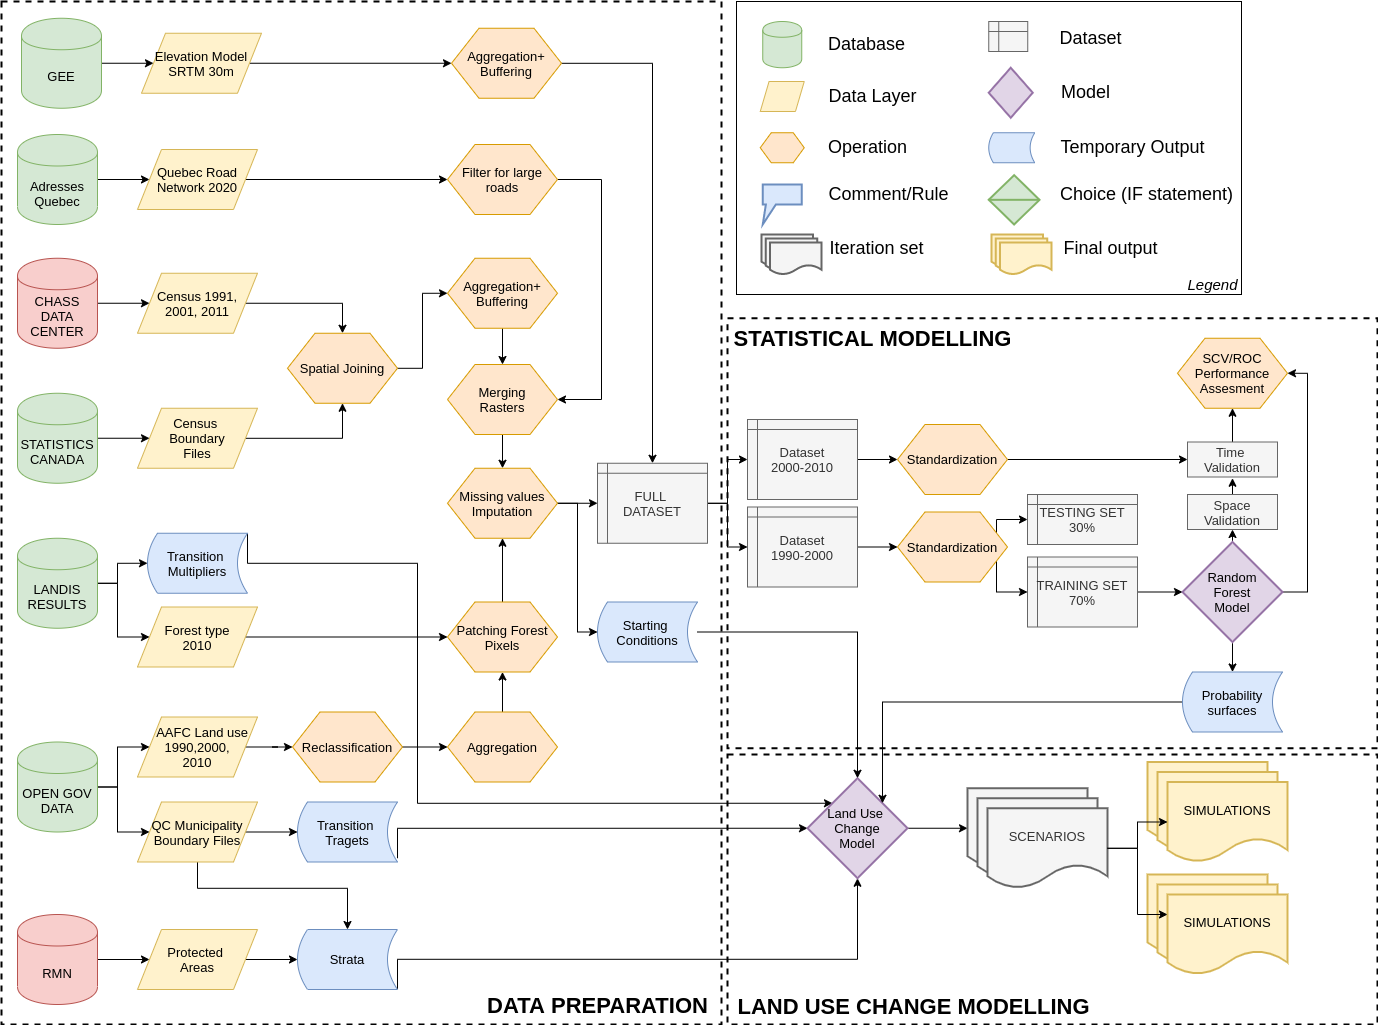
\includegraphics[width=1.25\textwidth]{thesis/figures/Chapter1_flowchart.png}
}
\caption[Workflow diagram for Chapter 1 (part 1)]{Workflow diagram for Chapter 1 (part 1). This figure shows the methodological steps for data preparation, statistical modelling and land use change modelling. Data layers (parallelograms) were extracted from multiple databases (cylinders) and processed (hexagons) in order to produced the outputs (data tables and raster layers) used for statistical and land use change modelling. The resulting data table was split in test and train sets before runnig the random forest model. Note the multiple outputs of the land use change model which produced different simulations based on scenarios. }
\label{fig:workflow1}
\end{figure}
\clearpage

\begin{figure}[h!]
\makebox[\textwidth]{
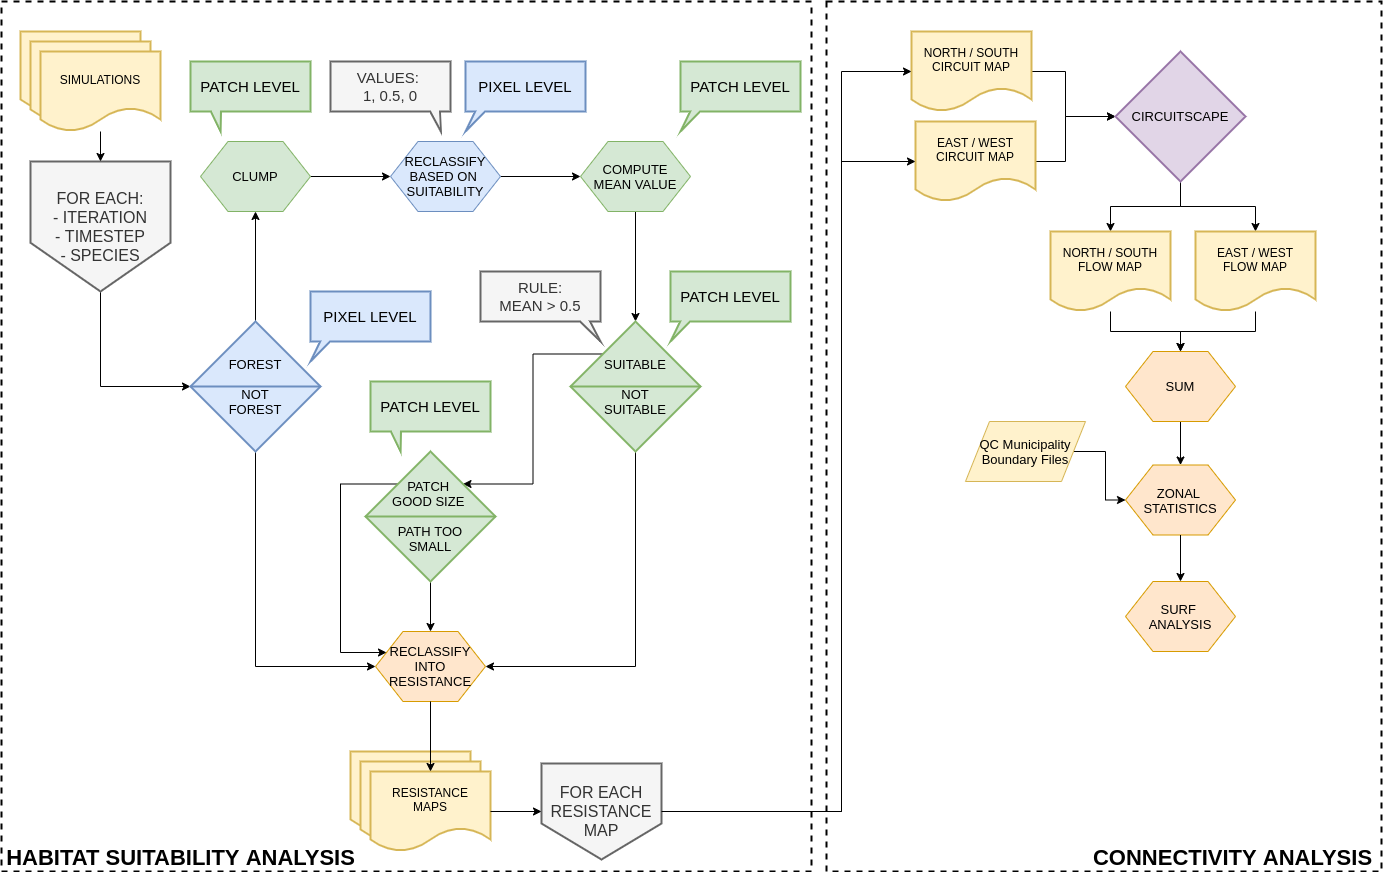
\includegraphics[width=1.25\textwidth]{thesis/figures/Chapter1_flowchart2.png}
}
\caption[Workflow diagram for Chapter 1 (part 2)]{Workflow diagram for Chapter 1 (part 2). We adapted the habitat suitabiliy anakysis steps from \cite{rayfield_priorisation_2018} to suit the characteristics of our data. From the land use change simulations results, we followed the steps outline on the left side. Either sides of "if statements" (rhombi) lead to different processing decisions (for instance, the size of suitable patches is evaluated before being reclassified into resistance, while unsuitable patches get the same resistance value for a given species). Note the different color denoting whether the processing step was performed at the patch level or at the pixel level. On the right side, the main steps of the connectivity analysis are represented: Curcuitscape is ran in two directions and the sum of these two outputs is taken to produce zonal statistics and proceed to the feature detection analysis (SURF analysis).} 
\label{fig:workflow2}
\end{figure}
\clearpage

%--------------------------------------------------------------------------------------------------
% Results figures

% Model tables (roc curves moved to the appendix)

% RF Variable importance

\begin{table}[h!]
\centering
\caption[Variable importance (gini impurity index) for variables in the random forest models]{Variable importance (gini impurity index) for variables in the random forest models - categorical variables are excluded (rounded to nearest integer, highest values are in bold).}
\label{tab:varimp}
\begin{tabular}{lcc}
\hline
\hline
\multicolumn{1}{c}{\multirow{2}{*}{Variable}} & \multicolumn{2}{c}{Model} \\ \cline{2-3} 
\multicolumn{1}{c}{} & \multicolumn{1}{l}{Urbanisation} & \multicolumn{1}{l}{Agricultural expansion} \\ \hline
Distance from urban land & \textbf{2118} & 571 \\
Size of forest patch & 409 & \textbf{8424} \\
Elevation & 184 & 796 \\
Population change & 332 & 297 \\
Income & 371 & 315 \\ 
\hline
\end{tabular}
%\end{table}

% R squares and AUC

%\begin{table}[!htbp] \centering 
  \caption[$R^{2}$, AUC, and average precision values for both models and both validation sets.]{$R^{2}$, AUC (Area Under Curve), and average precision values for both models and both validation sets - The spatial validation set corresponds to the testing partition for the 1990-2000 timestep, whereas the temporal validation set corresponds to the entire data of the 2000-2010 timestep.} 
  \label{tab:R_squares_AUC} 
\begin{tabular}{@{\extracolsep{5pt}} ccccc} 
\\[-1.8ex]\hline 
\hline \\[-1.8ex] 
Model & Validation set & $R^{2}$ & AUC & Average Precision \\ 
\hline \\[-1.8ex] 
Agricultural Expansion & Spatial & $0.566$ & $0.931$ & $0.652$ \\ 
Agricultural Expansion &  Temporal & $0.566$ & $0.841$ & $0.023$ \\ 
Urbanization & Spatial & $0.573$ & $0.939$ & $0.234$ \\ 
Urbanization & Temporal & $0.573$ & $0.921$ & $0.250$ \\ 
\hline \\[-1.8ex] 
\end{tabular} 
%\end{table} 

% R square resample

%\begin{table}[!htbp] \centering 
\caption[AUC values for both models in resampled 10 folds CCV]{AUC (Area Under Curve) values for both random forest models in resampled 10 folds CCV (Classic Cross-Validation).} 
\label{tab:R_squares_resample} 
\begin{tabular}{@{\extracolsep{5pt}} cccccc} 
\\[-1.8ex]\hline 
\hline \\[-1.8ex] 
Model & Mean AUC +/- Std \\ 
\hline \\[-1.8ex] 
Agricultural Expansion & $0.929 \pm 0.002$ \\ 
Urbanisation & $0.938 \pm 0.002$ \\ 
\hline \\[-1.8ex] 
\end{tabular}
%\end{table} 

% Historic model metrics

%\begin{table}[!htbp] \centering
\caption[AUC and average precision values for the predictions of the land use change model]{AUC (Area Under Curver) and average precision values for the predictions of the land use change model. A binary raster (transition either happened or did not happen) was used to generate those values.} 
\label{tab:historic_metrics} 
\begin{tabular}{lcccc}
\hline
\hline
\multicolumn{1}{c}{Model} & \begin{tabular}[c]{@{}c@{}}Mean AUC\\ (Averaged \\ Surface)\end{tabular} & \begin{tabular}[c]{@{}c@{}}Mean Precision\\ (Averaged \\ Surface)\end{tabular} & \begin{tabular}[c]{@{}c@{}}Mean AUC +/- Std\\ (All Iterations \\ Averaged)\end{tabular} & \begin{tabular}[c]{@{}c@{}}Mean Precision +/- Std\\ (All Iterations \\ Averaged)\end{tabular} \\ \hline
\begin{tabular}[c]{@{}l@{}}Agricultural \\ Expansion\end{tabular} & $0.858$ & $0.383$ & $0.678 \pm 0.002$ & $0.109 \pm 0.002$ \\
Urbanisation & $0.784$ & $0.287$ & $0.647 \pm 0.001$ & $0.135 \pm 0.001$ \\ \hline
\end{tabular}
\end{table}

%--------------------------------------------------------------------------------------------------
% Historic model 

\begin{figure}[h!]
\makebox[\textwidth]{
  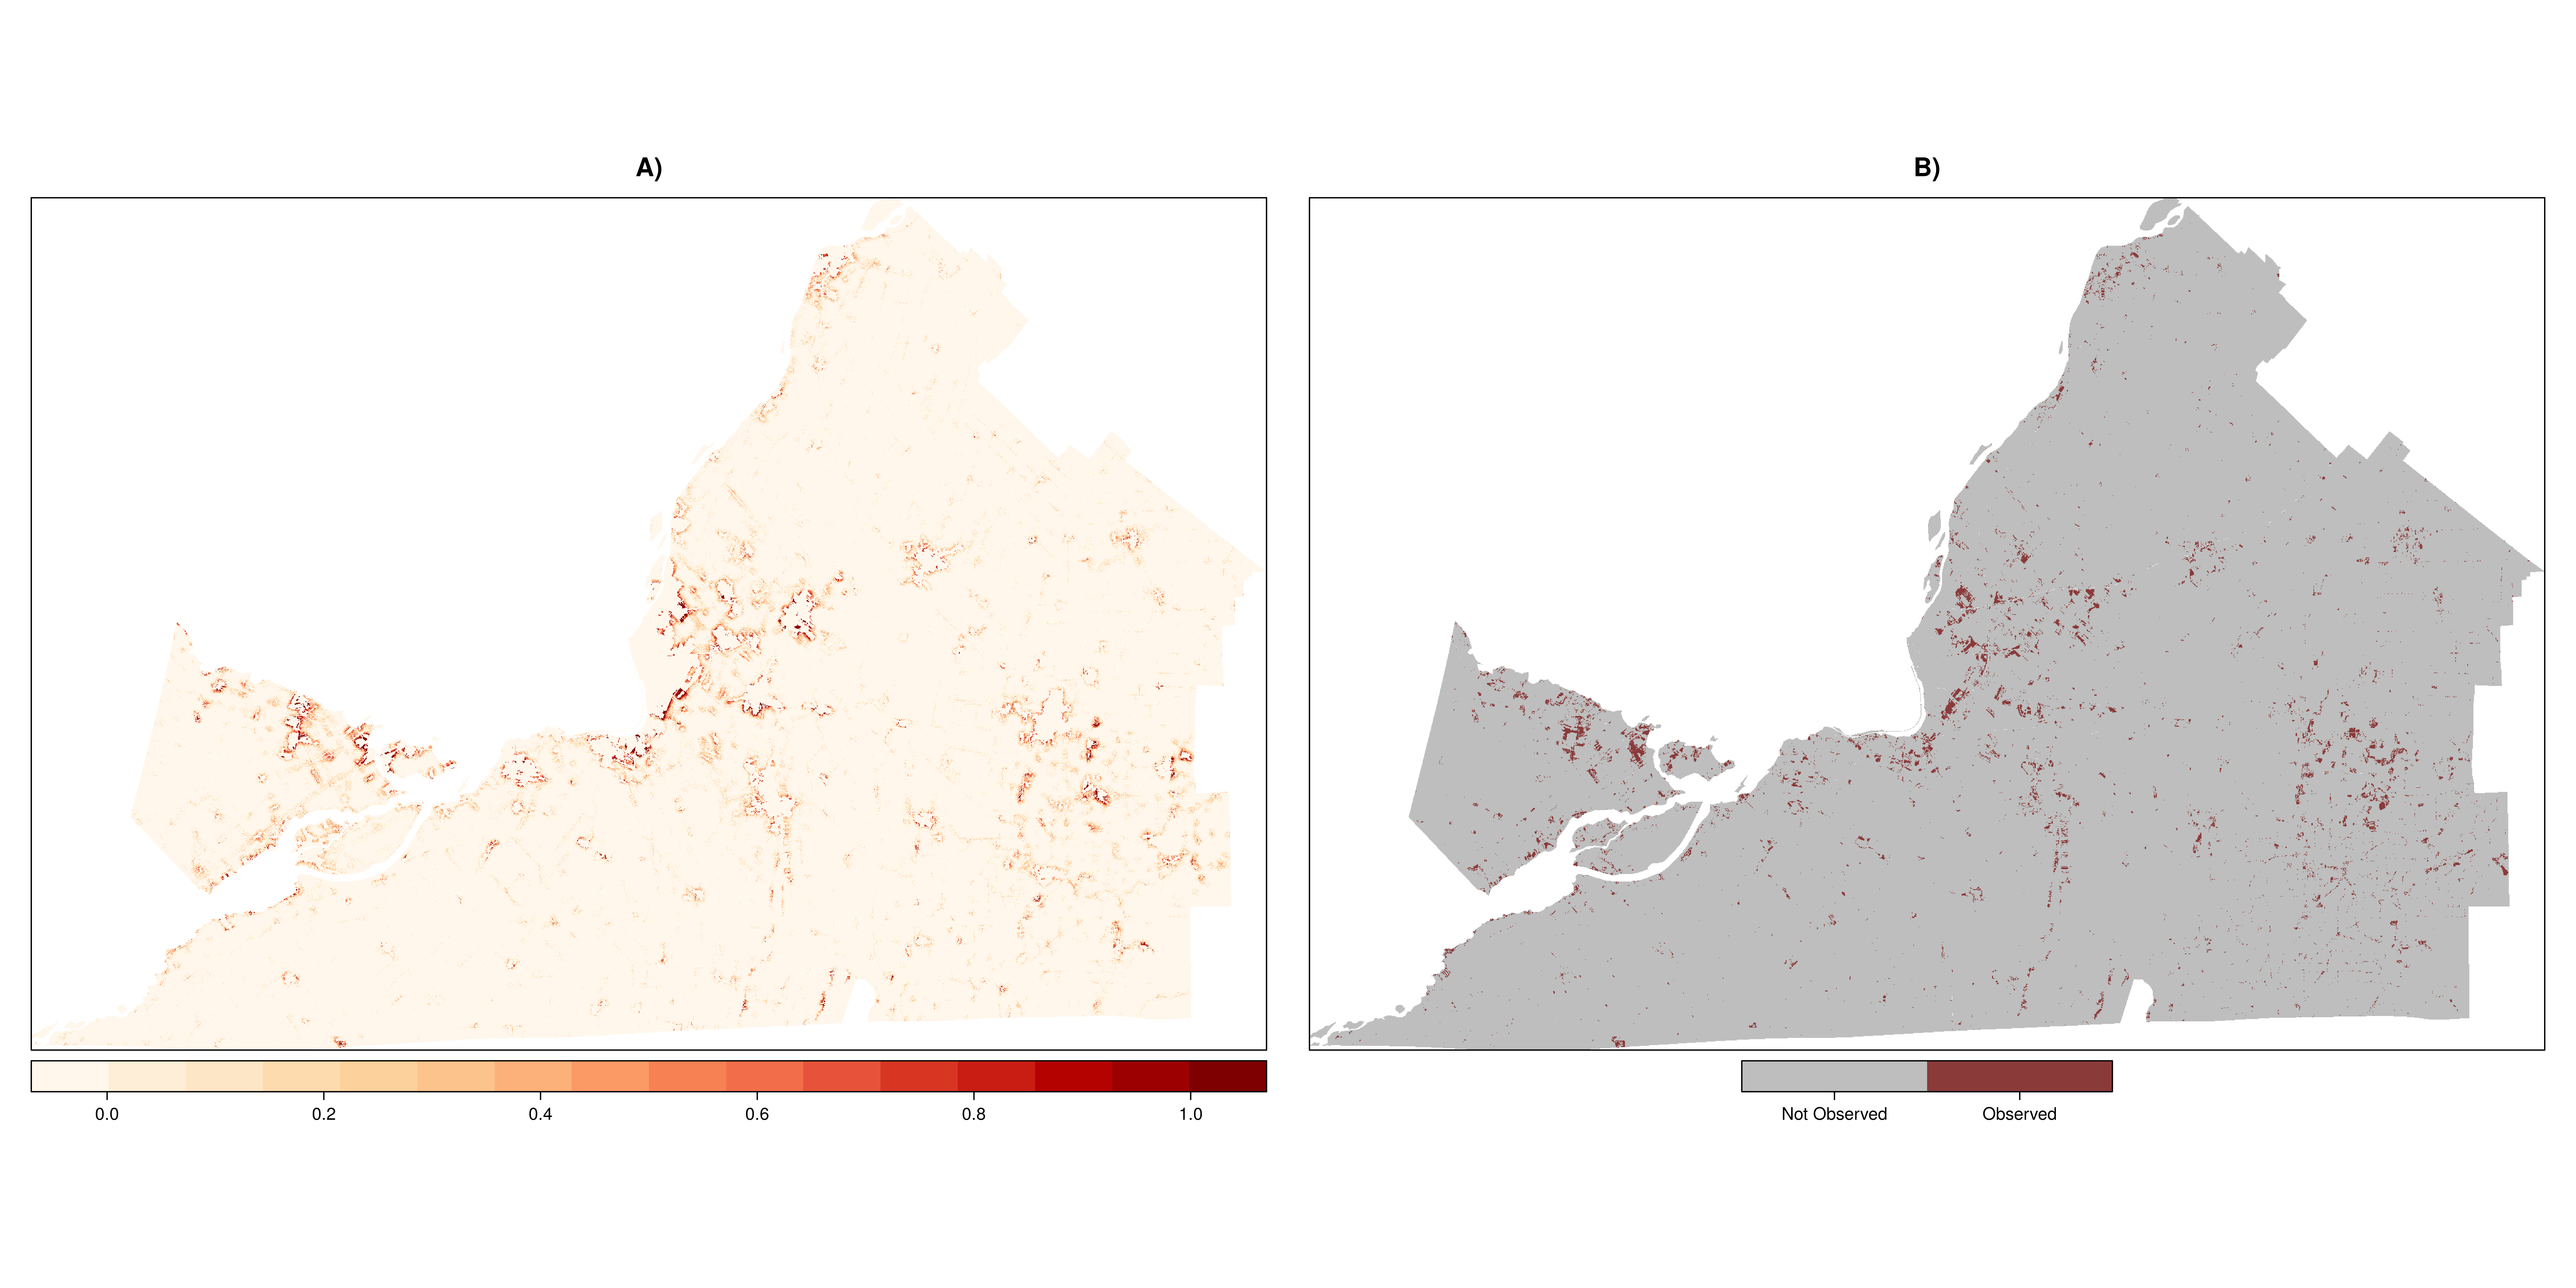
\includegraphics[width=1.2\textwidth]{thesis/figures/historic_compare_urb.png}
}
 \caption[Predicted probability of urbanization vs observed urbanization between 1990 and 2010.]{(A, left) Predicted probability of urbanization (deom 0 to 1) based on the Random Forest Model. (left) ; (B, right) Binary map (0 or 1, Not Observed OR Observed) for urbanization in Montérégie between 1990 and 2010. A near perfect model prediction would produce nearly identical maps.}
 \label{fig:compare_urb}
%\end{figure}

%\begin{figure}[h!]
\makebox[\textwidth]{
  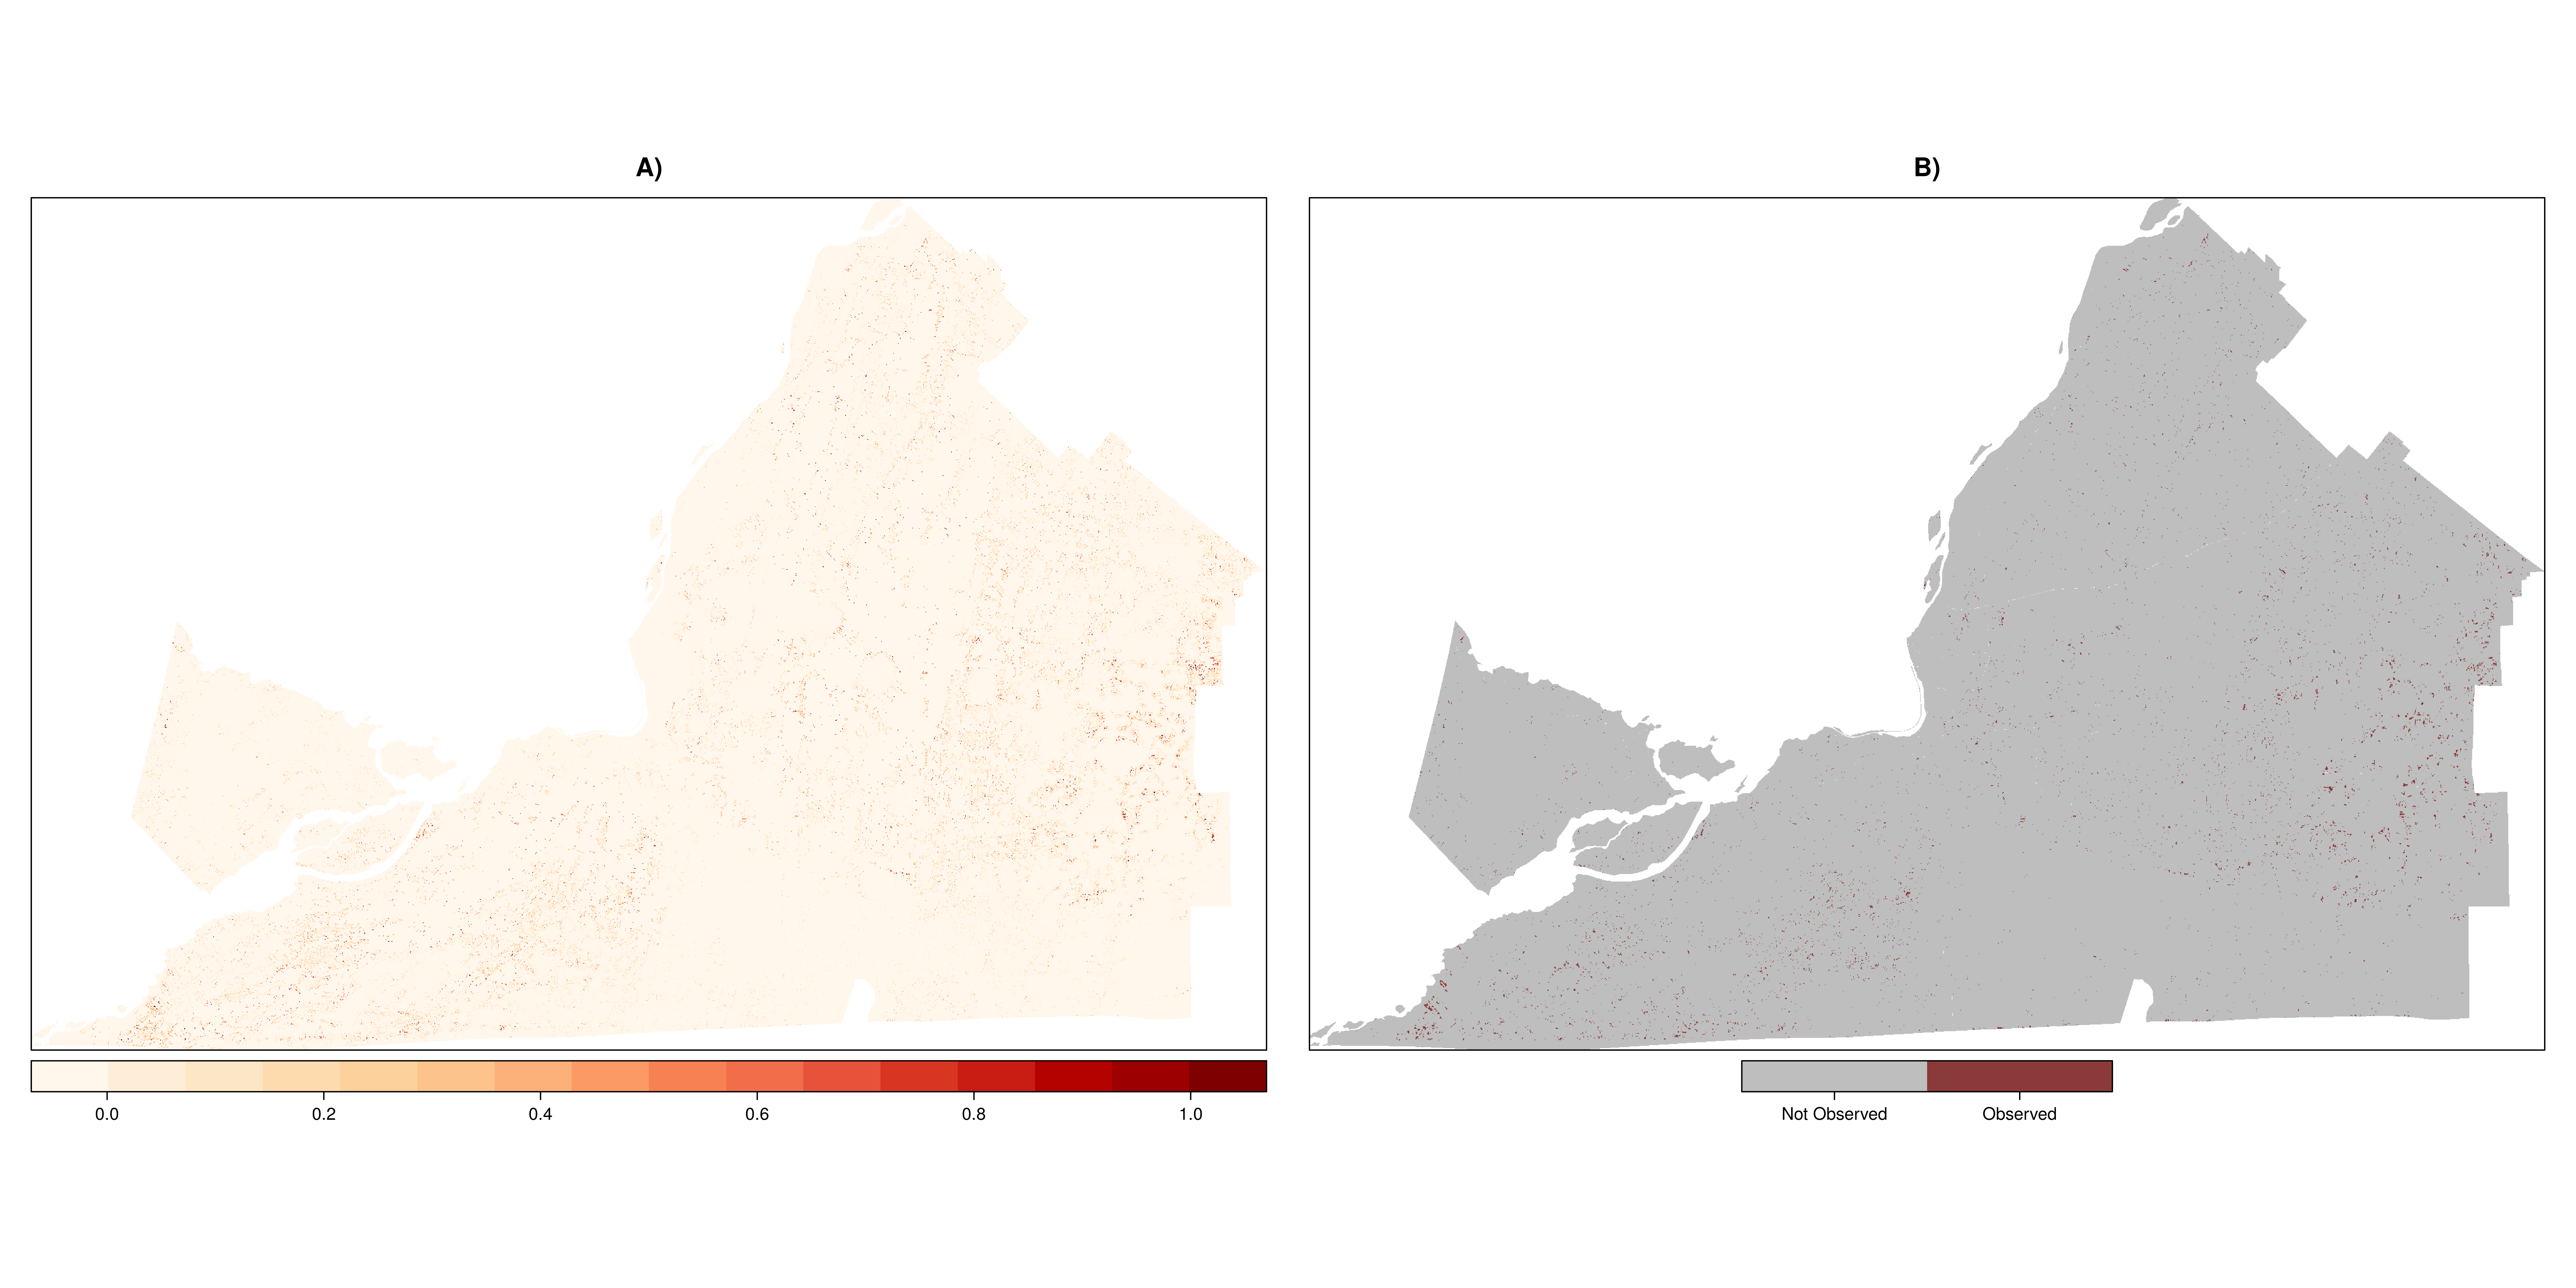
\includegraphics[width=1.2\textwidth]{thesis/figures/historic_compare_agex.png}
}
 \caption[Predicted probability of agriculral expansion vs observed agriculral expansion between 1990 and 2010.]{(A, left) Predicted probability of agriculral expansion (from 0 to 1) based on the Random Forest Model. (left) ; (B, right) Binary map (0 or 1, Not Observed OR Observed) for agriculral expansion in Montérégie between 1990 and 2010. A near perfect model prediction would produce nearly identical maps.}
 \label{fig:compare_agex}
\end{figure}

%--------------------------------------------------------------------------------------------------
% Other land use change scenario (maps moved to appendix)

\begin{figure}[h!]
\makebox[\textwidth]{
  \includegraphics[width=1.2\textwidth]{thesis/figures/bar_both.png}
}
 \caption[Land use class fequencies in 2010 and 2100 for the BAU and Reforestation scenarios ]{Land use class fequencies (in hectares) in 2010 (observed from the land use data) and 2100 (predicted by the land use change model) for the BAU (Business As Usual) and Reforestation scenarios (Note: these predictions are done under baseline climate scenario). Top: Forest broken down by forest types (coniferous, deciduous and mixed) ; Bottom: Agriculture and Urban.}
 \label{fig:bar_both}
\end{figure}

%--------------------------------------------------------------------------------------------------
% Histogram historic

\begin{figure}[h!]
\makebox[\textwidth]{
  \includegraphics[width=1.3\textwidth]{thesis/figures/original_hists.png}
}
 \caption[Histograms of flow values for 2010 comparing the historic model run (1990-2010) with observations]{Histograms of flow values (results of Circuitscape runs for study region) for the year 2010. This compares the current values from the output of the historic model (in blue, i.e. connectivity analysis of the output for the year 2010, after running the land use change model from 1990 to 2010) with the current values observed (in red, connectivity analysis of the observed land use maps in 2010).}
 \label{fig:hist_historic}
\end{figure}

%--------------------------------------------------------------------------------------------------
% Flow

% Historic

\begin{figure}[h!]
\makebox[\textwidth]{
  \includegraphics[width=1.3\textwidth]{thesis/figures/connectivity_decrease_x5species_historic.png}
}
 \caption[Change in mean flow (in \% of the 1990 flow) between 1990 and 2010, comparing the historic model run (1990-2010) with observations] {Change in mean flow (decrease in \% of the baseline 1990 flow) between 1990 and 2010. This compares the changes (decrease in current flow from the 1990 baseline) observed in the land use data (in blue), with the changes observed in the output of the historic model (ran from 1990 to 2010, in orange), facetted by species.}
 \label{fig:flow_historic}
\end{figure}

% Linear

\begin{figure}[h!]
\makebox[\textwidth]{
  \includegraphics[width=1.3\textwidth]{thesis/figures/connectivity_decrease_x5species_chap1.png}
}
 \caption[Linear graph of change in mean flow (decrease in \% of the baseline 2010 flow) between 2010 (observed) and 2100 (predicted), comparing BAU scenario with other land use change scenarios]{Linear graph of change in mean flow (decrease in \% of the baseline 2010 flow) between 2010 (observed) and 2100 (predicted). This compares the BAU (Business As Usual) scenario with the Reforestation (R) scenario, facetted by species. Note that the line type represents the different climate scenarios so as to represent all scenario combinations.}
 \label{fig:flow_linear_1}
\end{figure}

% Radar

\begin{figure}[h!]
\makebox[\textwidth]{
  \includegraphics[width=1.3\textwidth]{thesis/figures/radar_ggradar_chap1.png}
}
 \caption[Radar graph of change in mean flow (decrease in \% of the baseline 2010 flow) between 2010 (observed) and 2100 (predicted), comparing BAU scenario with other land use change scenarios]{Radar graph of change in mean flow (decrease in \% of the baseline 2010 flow) between 2010 (observed) and 2100 (predicted). This compares the BAU (Business As Usual) scenario with the Reforestation (R) scenario, for all 5 species. Note that the line color represent species and that each side of the graph is a different scenario combination.}
 \label{fig:flow_radar_1}
\end{figure}

% Histograms

\begin{figure}[h!]
\makebox[\textwidth]{
  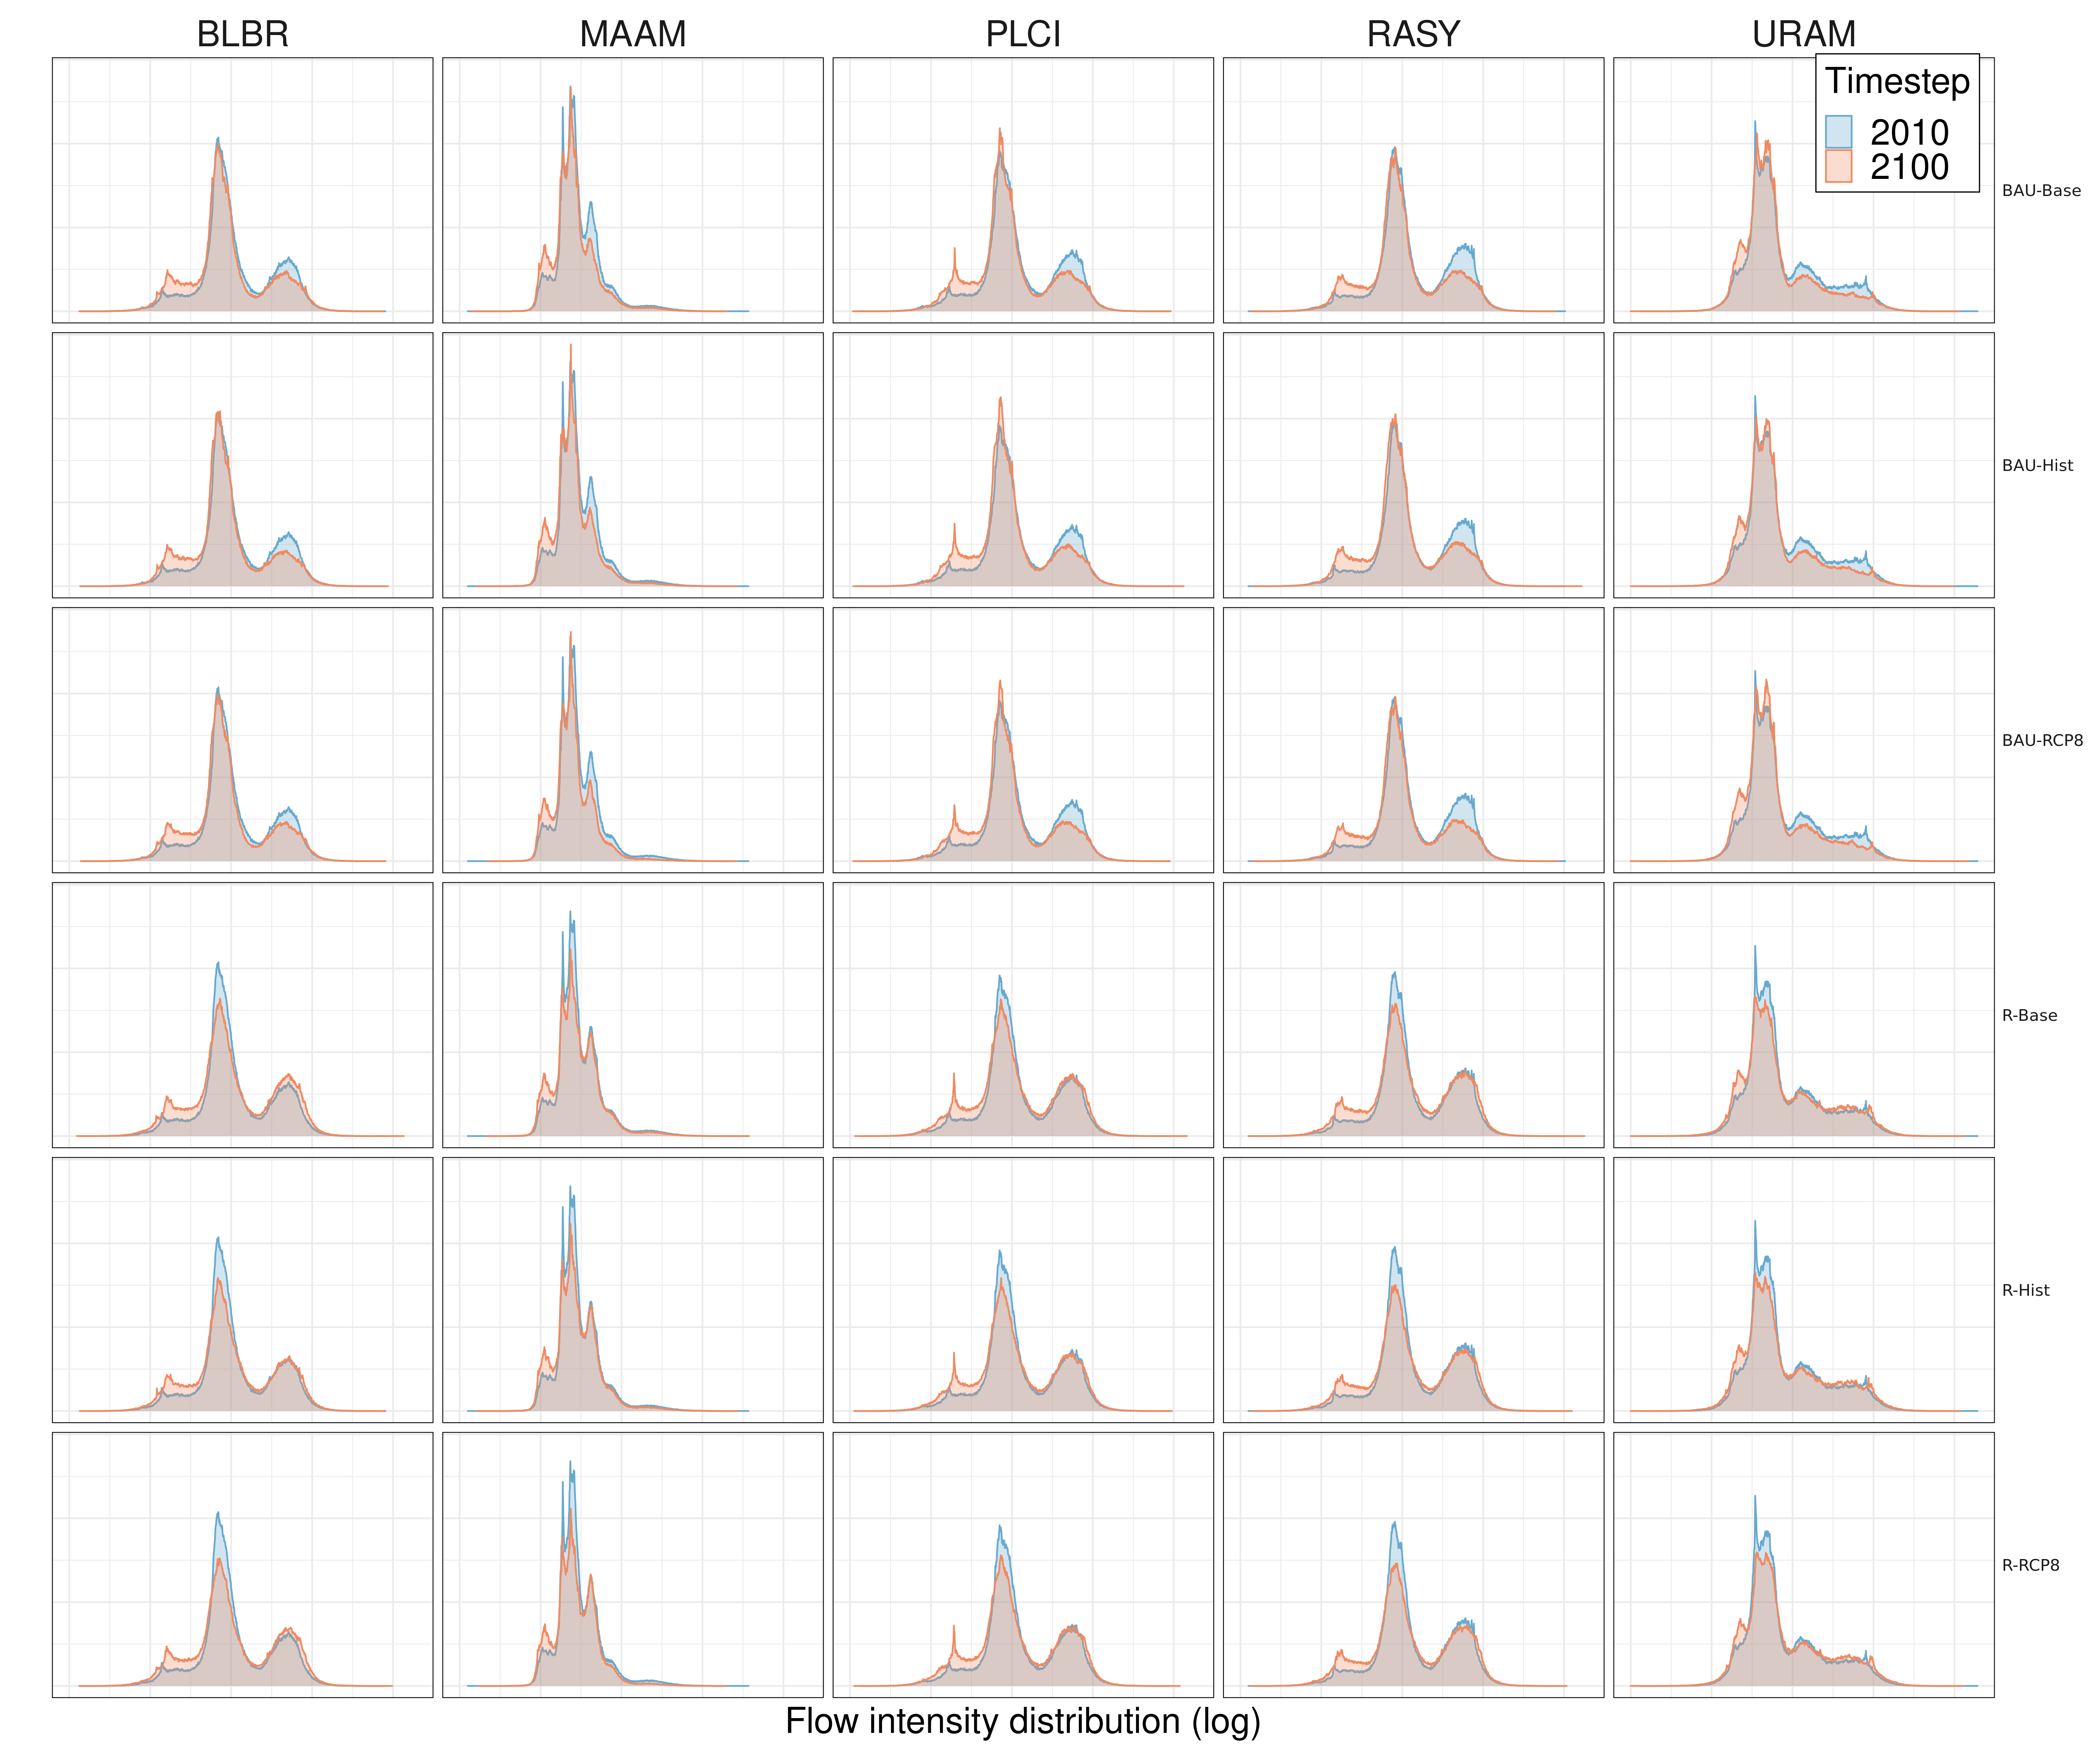
\includegraphics[width=1.3\textwidth]{thesis/figures/hist_chap1.png}
}
 \caption[Histograms of flow values for all species and scenarios, comparing timesteps 2010 (observed) with 2100 (predicted)]{
 Histograms of flow values (results of Circuitscape runs for study region) for the years 2010 and 2100. This compares the observed values for the year 2010 (in blue, i.e. connectivity analysis of the land use map) with the current values of the model output in 2100 (in red, connectivity analysis of the year 2100 of the output of the land use change model). Note that the results are facetted by species and by scenario combination.}
 \label{fig:hist_1}
\end{figure}

%--------------------------------------------------------------------------------------------------
% SURF

% Linear

\begin{figure}[h!]
\makebox[\textwidth]{
  \includegraphics[width=1.3\textwidth]{thesis/figures/surf_chap1.png}
}
  \caption[Linear graph of change in the number of features (decrease in \% of the baseline 2010 numbers) between 2010 (observed) and 2100 (predicted), comparing BAU scenario with other land use change scenarios]{Linear graph of change in the number of features (decrease in \% of the baseline 2010 numbers) between 2010 (observed) and 2100 (predicted). This compares the BAU (Business As Usual) scenario with the Reforestation (R) scenario, facetted by species. Note that the line type represents the different climate scenarios so as to represent all scenario combinations.}
 \label{fig:surf_linear_1}
\end{figure}

% Radar

\begin{figure}[h!]
\makebox[\textwidth]{
  \includegraphics[width=1.3\textwidth]{thesis/figures/surf_radar_chap1.png}
}
  \caption[Radar graph of change in number of features (decrease in \% of the baseline 2010 numbers) between 2010 (observed) and 2100 (predicted), comparing BAU scenario with other land use change scenarios]{Radar graph of change in number of features (decrease in \% of the baseline 2010 numbers) between 2010 (observed) and 2100 (predicted). This compares the BAU (Business As Usual) scenario with the Reforestation (R) scenario, for all 5 species. Note that the line color represent species and that each side of the graph is a different scenario combination.}
 \label{fig:surf_radar_1}
\end{figure}

%\begin{figure}[h!]
%\makebox[\textwidth]{
%  \includegraphics[width=\textwidth]{figures/.png}
%}
% \caption{}
% \label{fig:}
%\end{figure}

\printbibliography[heading=bibintoc, section=1, title={Chapter 1 Bibliography \hspace{1em}}]

\endrefsection

\newpage


\SetLinkName{Linking Statement}
\SetLinkText{In Chapter I, we integrated a land use model and a climate change model with a habitat suitability and connectivity model. We then explored outcomes under different scenarios for land use and climate change. We showed how different species might react to changes in land use and climate by analyzing the resulting flow surfaces. We provided  a reproducible yet perfectible methodology that takes into account important drivers like land use and climate change. We applied these methods to the case of the Montérégie in Québec. We demonstrate the power of simple scenarios to identify the boundaries of the prediction space for potential functional connectivity. However, we recognize the need for scenarios that take into account the needs and perceptions of stakeholders of the region. In Chapter 2, we take a first step toward deriving the basis for such community-driven scenarios by presenting the results of a community workshop organized between multiple stakeholders in Montérégie. We use those results to derive simple land use change scenarios and use those scenarios to constrain the integrated model from Chapter 1. These scenarios can serve as a basis with which to iterate a community-driven process of conservation scenario building. We derive the same analysis for the species described in Chapter 1 and compare and contrast the results between scenarios. This integrated approach has the potential to support ongoing connectivity conservation planning in the south of Québec.}
\Link

%  Chapter 2
% !TEX root = ./thesis.tex
\chapter{Integrating Stakeholders Perceptions of Connectivity Conservation Priorities into a Spatially Explicit Land Use and Connectivity Change Model}
\begin{center}
{Valentin Lucet$^{1}$, Andrew Gonzalez$^{1}$}\\
\end{center}
\textit{Author Affiliations:}\\
\normalsize{$^{1}$Department of Biology, McGill University}\\

\newrefsection

\section{Abstract}

Connectivity conservation science, whose goal is to preserve the continuity of habitat throughout a given landscape, proceeds by identifying priority areas given the current configuration of the landscape. However, current connectivity conservation planning methods often do not confront the results of the prioritization with the priorities perceived by stakeholders. There is a need for planning tools to allow for this confrontation to happen. The Montérégie region in southern Québec, where this work takes place, is experiencing urban growth and sprawl, and stakeholders show an increasing interest in connectivity conservation tools. Those tools need to be able to guide stakeholders through an iterative process of conservation and land use scenario building. We take a first step toward deriving the basis for such community-driven scenarios and tools by presenting the results of a community workshop organized between multiple stakeholders in Montérégie. We use those results to derive simple land use change scenarios and use those scenarios to constrain the integrated model previously derived. We discuss the importance of considering stakeholder inputs to produce a resilient network of protected areas and highlight the need for a multi-stakeholder approach in the definition of conservation priorities. \\

\newpage

\section{Introduction}

% Intro paragraph, similar to that of from chapter 1

The goal of connectivity conservation planning is to preserve the continuity of habitat in a landscape, by identifying and protecting habitat patches and corridors necessary to maintain the movement of plants and animals \citep{keeley_thirty_2019}. Ecological connectivity, defined as the extent to which the landscape facilitates or impedes the movement of organisms \citep{crooks_landscape_2006}, is a critical component of the resilience of populations in heterogeneous and fragmented landscapes \citep{gonzalez_spatial_2017}. Connectivity conservation planning methods do not typically account for, nor contrast the perceptions of stakeholders as they relate to  their priorities for conservation. Here, we ask how methods in connectivity conservation can take into account stakeholder perceptions. To do so, we integrate a connectivity and land use change model (developed in chapter 1) with the results of a community workshop organized with stakeholders, through simple conservation scenarios.

Conservation planning methods are now recognizing that landscapes constitute social-ecological-systems. A social-ecological system (SES) can be understood as the ensemble of human and non-human actors in a given landscape, the set of natural habitats they inhabit and resources they use, and the set of interactions that are maintained between all the components of the system \citep{ostrom_general_2009}. SESs thus form complex and integrated aggregates of interactions \citep{hinkel_enhancing_2014}. Those interactions also impact governance, the process by which actors in power establish rules and laws \citep{bissonnette_comparing_2018}. To understand a landscape as an SES has important implications for land use planning and therefore for connectivity conservation planning, and pushes connectivity scientists to integrate stakeholder’s perceptions and priorities into their models. 

It is important to integrate the perceptions of stakeholders in connectivity planning methods for a number of reasons. It engages stakeholders in the planning process early on, contributing to better consensus on priorities and, hopefully, to faster action. It also means that connectivity models are enriched by integrating local knowledge into the decision making process, showing that inputs from stakeholders are valued and considered essential to build a conservation plan. More specifically, connectivity conservation is often faced with the issue of understanding the processes driving land use change \citep{worboys_connectivity_2010}. Because land use change is a social process with consequences of both social and ecological nature, questions of land use and connectivity planning cannot be answered without input from stakeholders. Recent studies in land use modelling have shown the value of using stakeholder’s inputs for parameterizing and validating models \citep{hewitt_participatory_2014, voinov_modelling_2010}, leading to a much better understanding of land use processes at play within a landscape.

Connectivity conservation research therefore has a lot to gain from the wide set of participatory research methods already being used in social-ecological research. Participatory research methods are designed to conduct the research process “with those people whose life-world and meaningful actions are under study” \citep{bergold_participatory_2012}. Participatory research methods can include scenario design. A scenario is “an account of a plausible future” \citep{peterson_scenario_2003}, and scenario design is a flexible tool for conservation scientists and practitioners. Although scenarios are often derived from expert knowledge, they can be built in a participatory setting. In this context, it is often conceived by researchers as an iterative process, through which scenarios are imagined, reviewed and re-imagined in a set of stakeholder meetings with the goal to build consensus on the desirability of each scenario. 

Scenarios have been widely applied in conservation research, both at global \citep{tscharntke_global_2012, brussaard_reconciling_2010}, regional and local \citep{carlson_scenario_2011, delevaux_scenario_2018} scales. In a participatory setting, other methods can be used to help in scenario design: those methods include participatory mapping, a participatory GIS method. Participatory mapping involves leveraging the knowledge that stakeholders hold about the geography of their landscape, in order to achieve a community-driven objective. It has been widely used in social-ecological research \citep{plieninger_assessing_2013, lynam_review_2007}. 

Participatory GIS methods such as participatory mapping can allow connectivity conservation models to be more spatially explicit about the obstacles and opportunities presented by connectivity conservation. Understanding how these obstacles and opportunities can influence management decisions is crucial for our understanding of connectivity conservation planning, where land-use conflicts can hinder the protection and restoration of connectivity. Although it is relatively easy to identify where land-use changes might conflict with connectivity conservation, evaluating to which extent these conflicts matter in a local conservation context is more difficult \cite{mitchell_monteregie_2015}.

Here, we do not present a scenario design exercise, but a community workshop with a consensus building and participatory mapping exercise, whose results were translated into simple scenarios in an integrated land use, climate change, and connectivity model (developed in chapter 1). We improve our understanding of the obstacles and opportunities to connectivity conservation in the region, and provide a good starting ground for an iterative process of scenario building. We focused on the region of Montérégie, in southern Québec, where connectivity conservation has become the focus of land use planning decisions. This project has been developed in collaboration with the non-profit NAQ (Nature action Québec) in the context of a multi-stakeholder conservation project, the PADF (Plan d’Aménagement Durable des Forêts). The PADF aims at building consensus on priorities for the management and possible conservation of forested land in the region.

This research is an extension of the work initiated by the project “Montérégie Connection”, whose goal was to engage stakeholders around a discussion of the ecosystem services provided by natural habitat in the region. In the context of this stakeholder-driven project, \cite{mitchell_monteregie_2015} conducted a non-spatially explicit scenario building exercise for a subset of the Montérégie region, the Vallée-de-Richelieu Municipalité Region Comté. The outcome was 4 scenarios, ranging from “Periurban Development” to “Green Development”, and each describing different land use change trends. The Montérégie connection project improved our understanding of the relationship between forest connectivity and ecosystem services. However, there was no effort to estimate the impact of each scenario on ecological connectivity. This is partially due to a lack of tools able to translate these scenarios into simulations. We contribute to the development of such tools by integrating the results of the workshop into the land use change model developed in chapter 1. The goal of this chapter is therefore twofold: gain a better understanding of conservation priorities in the region, and to provide a basis for an iterative scenario-building process. \\
%-----------------------------------------------

\section{Methods}

In order to understand what stakeholders perceive as a conservation priority, and derive conservation scenarios from those perceptions, we conducted a community workshop. The workshop was approved by McGill University’s Research Ethics Board (see Appendix 2 for the approval letter). The workshop was held on January 22nd 2020 in the public library of Saint-Jean sur Richelieu. \\

\subsection{Community workshop}

The workshop aimed to gather stakeholders from multiple groups:
\begin{enumerate}
  \item Representatives of Non-Governmental Organizations that are involved in the conservation of ecological connectivity within the study extent (i.e. Montérégie).
  \item Land use planners (“amenagistes”) of the administrative regions covered by the study extent (the 15 MRCs in Montérégie).
  \item Representatives of Ministries involved in conservation (MFFP, MELCC).
  \item Representatives of the UPA (“Union des producteurs agricoles”) in Montérégie.
  \item Representatives of the private forestry industry unions (“producteurs forestiers”)
\end{enumerate}
Of all the groups, only the last group was not represented. \\

\subsubsection{Consensual mapping}

We employed a method coined “consensual participatory mapping in geographically structured focus groups”. Participants whose organisations operate in the same region (the same MRC) were seated at the same table. See table \ref{tab:workshoptables} for the breakdown of each MRC by table. In addition, for participants whose zone of influence or zone of action covered the whole region, two “regional tables” were created. In the subsequent sections, the workshop results are divided between the regional and regional tables.
The general method proceeded in 3 exercises, each step involving the same focus groups.

\begin{itemize}
  \item Exercise 1: mapping of forested cores of importance for ecological connectivity.
  \item Exercise 2: mapping of obstacles (for example: specific land use types, development projects in progress, local legislation) and opportunities for habitat connectivity in terms of social-economic activity and land use.
  \item Exercise 3: mapping of links (already recognized or potential) of importance between forested cores of importance, taking into account obstacles and opportunities on the landscape.
\end{itemize}

Each of these three exercises was conducted in 4 to 5 steps. Here we use exercise 1 to describe the method in more detail at each step.

\begin{enumerate}
\item Individual reflection - each participant thought on their own about the problem at hand. For instance, participants took time to think about what forested cores are important to connect in the landscape
\item Group discussion, at each table (i.e. in each focus group) each participant contributed their answer to the question posed by the exercise. For instance, participants shared what forested cores they found to be important.
\item Group discussion on the criteria that each participant used to answer the question. For instance, participants said why they thought they chose these forested cores.
\item Consensus building, participants voted for the most important criteria. For instance, participants used stickers that identify their group affiliation to vote for the criteria they found most important.
\item Room discussion: all participants exchanged on their decisions by sharing the results of their table’s work to the rest of the room.
\end{enumerate}

Each participant received a unique and neutral identifier of the form Affiliation-Geography. For example, a (hypothetical) land use planner from the table that brought together participants from the Maskoutains region received the code [A-1-1], and the UPA representatives from the Richelieu region received the codes [C-3-1] and [C-3-2]. In addition, for certain activities, the affiliation of the participants is color-coded. For instance, blue for the land use planners and purple for the ministry representatives.

The coding system manifests itself in multiple ways, depending on the activity:
\begin{itemize}
\item When participants engage in activities involving drawing, the materials on which they draw will bear the aforementioned coding (A-1 etc..).
\item When participants engaged in activities involving post-its, the color of their post-it represented their affiliation or bore the aforementioned coding, depending on the activity.
\item When participants engaged in activities involving a weighting of choices with stickers, the color of their post-it or sticker represented their affiliation or had the aforementioned coding, depending on the activity.
\end{itemize}

To ensure that this system is used consistently throughout the workshop, each participant was given a personal folder with their own color-coded stickers and post-its. Participants were instructed to only use the stickers and material that have been personally handed to them. All participants were given a visual aid to remind them of the agenda of the workshop. Facilitators were also present at almost every table and helped facilitate the discussion. They were given a document to help them in this role. The workshop materials, including the ethics approval document for this research project can be found in Appendix 2.\\

\subsubsection*{Weighting system}

The participants were given a total of 6 stickers to cast their vote for the opportunities and obstacles that they thought were most important. They were given a total of 6 stickers: 2 blue (important), 2 yellow (very important) and 2 red (of the first importance).\\

\subsubsection{Data processing and analysis}

\subsubsection*{Voting: opportunity and challenges}

The data from the opportunities and challenges activity (with post-its), and the weighting of these elements were treated with the following steps:
\begin{enumerate}
  \item Each post-it (opportunity or challenge) received a unique ID.
  \item A first score is calculated by summing the points for each sticker (each vote)
  \begin{itemize}
      \item 1 point for a blue vote
      \item 2 points for a yellow vote
      \item 3 points for a red vote
  \end{itemize}
  \item This score was then weighted by multiplying it by the post-it’s diversity score which served as a measure of consensus
\begin{itemize}
\item This diversity score is the inverse simpson index (R package Vegan). The more diverse the group the higher this index is.
\end{itemize}
\end{enumerate}
These steps were carried out for each table and the results were treated separately for each table because not all tables had the same potential for diversity. For each table, the 10 post-its with the highest scores were retained, 5 among the post-its that had been placed on a specific area of the map (spatialized) and 5 for those that were not. The list of post-it contents, along with the scores, can be found in the appendix tables \ref{tab:opp_chall_ns} and \ref{tab:opp_chall_s}. In addition, a map synthetic map of the spatialized post-its was produced (see figures \ref{fig:reg_AC} and \ref{fig:trans_AC}).\\

\subsubsection*{Digitization of results}

The priority areas and links were digitized by hand in QGIS. The smooth tool was used to generalize the trace of each area and corridors (see figures \ref{fig:reg}  and \ref{fig:trans} for the final results). It is important to note that those maps are an approximate representation of reality, as the drawings done during the activity were an approximation of what the participant had in mind.

In order to integrate the results with the land use change model, we added a 5 km buffer around the linkages to simulate a corridor effect. This corridor width size is arbitrary and is in most cases  an unrealistic expectation for how large a wildlife corridor can or should be. \\

\subsection{Conservation and land use change scenarios}

The conservation scenarios were derived with the goal to demonstrate how results of this type of community workshop can be integrated with other planning methods for connectivity conservation, such as land use change and connectivity modelling. They are not meant to be directly used as conservation guidelines. They are unrealistic by definition and are meant to reflect the most extreme bounds of connectivity change and/or protection measures imaginable for the region. More realistic scenarios featuring targeted action would need to be devised in future community workshops. Although there exists a tremendous amount of work on scenario-building for conservation, specific examples for connectivity conservation are rare. The scenarios presented here are a “proof of concept” for the integration of qualitative results into a quantitative model. 

We integrated the results of the workshop with the land use change and connectivity model devised in Chapter 1 by changing two attributes of the model: \textit{conservation status} and \textit{reforestation location}. These additional conservation scenarios are crossed with the climate change scenarios.

Conservation status determines whether or not forest can be cut down, and whether pixels can transition into urban and agricultural land. In Chapter 1, we gave this status to areas that were previously known as protected, but assumed no more forest would be added to this set of protected areas. In this chapter, a protection status is given to all pixels within the identified priority areas and within a 5km buffer around the identified priority linkage areas. All pixels under this status cannot transition into urban land and remain in their state. This represents an unrealistic proportion of the region under protection (about 33% of the region)

The reforestation status modified what zones can be targeted for reforestation. In reforestation scenarios in Chapter 1, reforestation happened randomly (barring some neighboring rules). In this chapter, reforestation is targeted to the same areas identified in the workshop (all pixels within the identified priority areas and within a 5km buffer around the identified priority linkage areas). As in the model described in Chapter 1, all new reforested areas take the value of medium aged (30-50 yr) deciduous forest and remain in this state for the rest of the simulation. As previously mentioned, this assumption is necessary because LANDIS surface types are not available for newly forested areas. For the same reason, no forest transitions are allowed for this forest type. These two assumptions are conservative:  we do not impose succession or disturbance on these newly forested areas and assume medium age as an average age class.

The three modified conservation and land use change scenarios are therefore:
\begin{enumerate}
  \item Business as usual land use change + corridor protection \textbf{(BAU-Corr)}
 \item Business as usual land use change + corridor protection + reforestation \textbf{(BAU-R-Corr)}
 \item Business as usual land use change + corridor protection + targeted reforestation \textbf{(BAU-R(T)-Corr)} \\
\end{enumerate}

\subsubsection{Connectivity analyses}

In order to be able to compare the results of these new scenarios with those developed in Chapter 1, we conducted the same connectivity analyses using the Circuitscape software. The software “borrows algorithms from electronic circuit theory to predict connectivity in heterogeneous landscapes". It is a free and open software under MIT license developed originally in Python, and now in its 5th version, in Julia \citep{circuitjulia}.

For each of the maps produced in the suitability analysis, Circuitscape was run in two directions (“wall to wall” run, \cite{mcrae_conserving_2016}): east to west and north to south. This method allowed us to model omnidirectional animal movements, and required that we added the resulting North/South and East/West flow map. The results for each map were therefore added to produce a final set of flow maps for analysis. From these flow maps, we extracted the mean flow for each of the municipalities and for the entire flow map. 

In addition, similarly to in Chapter 1 we extracted the distribution (logged) of pixel flow values under the form of histograms. We also ran the SURF analysis in the same way and counted up the number detected feature for each surface, in order to derive a measure of flow complexity.\\

\section{Results}

\subsection{Community workshop}

During our community workshop, participants identified connectivity conservation priorities in Montérégie. Participants quickly built consensus on which key cores areas and corridors should be prioritized for protection or restoration. They mainly identified large forested regions and protected areas as key cores areas. As key corridors, participants were strongly drawn to linear strips of connecting “stepping-stone” patches. They were rarely drawn to redundant corridor design. When participants were asked what factors would make a link a priority, they emphasized the quality of habitats to be linked, as well as a diversity of constraining and facilitating factors.

Participants also workshopped constraints and assets to connectivity conservation in Montérégie. We divided the results into elements that had been spatialized (i.e. placed on a specific location of the map during the exercise), and non spatialized (i.e. not placed on a specific location), and scored them for the level of consensus they generated. Constraints scored higher, on average, than assets, indicating a focus of participants on constraints. The elements in the spatialized set scored higher on average than in the non spatialized set, indicating that participants tended to focus on more tangible and local issues and assets.

Non-spatialized elements seemed to speak to more general and large scale aspects. The main theme among these elements was predominance of agriculture in the landscape, and the difficulties to reconcile agricultural production with conservation. On the other hand, spatialized elements seemed to reflect local realities for connectivity conservation, such as the presence of highways or specific trends in land use change such as villegiative pressures. \\

\subsubsection{Forested cores of importance} 

Protected areas are well represented in the identified key core areas, for example the protected areas of the Green Mountains in the MRC of Brome-Missisquoi, or parts of the Monteregian Hills such as the Mount Saint-Hilaire. 

The participants at the sub-regional (figure \ref{fig:reg_AC}) and regional (figure \ref{fig:trans_AC}) tables identified redundant groups of forest patches. Because regional tables covered the whole of Montérégie, they often identified cores that contained the cores identified by the sub-regional table. \\

\subsubsection{Obstacles and assets}

The tables identified a total of 63 items as opportunities or assets, and 56 as constraints or obstacles. Tables \ref{tab:opp_chall_s} and \ref{tab:opp_chall_ns} displays the 5 assets or obstacles that scored the highest for each workshop table. 

Non-spatialized elements seemed to speak to more general and large scale aspects. Among them, the assets that scored the highest varied according to the sub-region under consideration. In the Centre table participants emphasized the strong presence of environmental NGOs, whereas the North and East tables emphasized elements linked to forest management. Interestingly, the presence of a strong agricultural matrix in the region scored high as an asset at the regional tables, and very high as a constraint on a sub-regional table, highlighting the polarizing status of the agricultural land use type in the region. Another constraint linked to agriculture is the CPTAQ - an agency responsible for the protection of agricultural lands often involved in discussions around land use planning - mentioned for the Centre sub-region. Similarly, the East table mentioned the issues that farmers have to make their farm profitable as another constraint. Besides agriculture, participants emphasized other constraints, such as economic realities making conservation a less likely investment, given the cost of implementing connectivity conservation measures - also mentioned as a perceived constraint. Finally, the participants mentioned that the overwhelming majority of forests are situated on private lands, along with the existing road infrastructure.

Spatialized elements seemed to reflect local realities for connectivity conservation. They are summarized in maps \ref{fig:trans_AC} and \ref{fig:reg_AC}, which shows the single highest scoring element (asset or constraints) for each sub region. the Centre, East and North tables mentioned positive local inclinations toward conservation. Similarly, the West and regional tables mentioned local legislation and the active mobilization of stakeholders, highlighting that connectivity conservation is a concern for many stakeholders in the region. Concerning constraints, participants emphasized once again elements related to the predominance of agriculture in the region. The lack of engagement from farmers was mentioned in the Centre and West tables, along with land use "pressures" coming both from agriculture and urban spread. The East table emphasized on the similar "villegiative" pressures, along with more local concern such as the Highway 10 and the intensity of local agriculture practices. The North table also mentions its highways. The regional tables mentioned the price of agricultural lands and the need for compensating the loss of agricultural production due to conservation. \\

\subsubsection{Links of importance at the regional scale}

\subsubsection*{Factors of priority}

Among the factors that were designated as a priority for the identification of links, participants emphasized the characteristics of the natural environments that make up the nodes that are to be connected. They mentioned the importance of the "quality" of these nodes themselve: for instance, the protection status of habitats, their diversity (variety of habitats), their surface area, isolation or proximity, and the pre-existence of connectivity potential. This highlights that stakeholders agree on the value of high quality habitats and on the need to protect them.

Participants debated the importance of both "facilitating" and "constraining" factors in deciding whether a link is a priority. Facilitating factors included the feasibility of establishing the link, social facilitators such as political and social buy-in, and territorial facilitators, such as appropriate land use. There were several types of constraints: financial, social, territorial and physical, and must be considered in relation to the socio-political and spatial planning context in which they emerge.

The presence of species at risk was identified as an important factor, along with other elements such as social factors (available economic means and the level of local interest in conservation) and characteristics of the link itself, including the functionality of the corridor. Consideration of threats such as the level of fragmentation was also noted. Finally, the fact that the environment is to be protected or restored was also deemed important. Interestingly, regulations are among the factors that were cited less often, such as Québec's PRMHH ("Plans régionaux des milieux humides et hydriques", or regional wetlands conservation plans), and migration routes. \\

\subsubsection*{Priority link mapping}

The consensual mapping process identified important links between the key areas identified in the previous steps at both sub-regional (figure \ref{fig:reg}) and regional tables (figure \ref{fig:trans}). At sub-regional tables, participants displayed what could be called "corridor opportunism": participants wanted to link areas by joining patches they judged to be organized in a linear or corridor-like fashion.

Participants were rarely drawn to redundant corridors. Tables were asked to limit themselves in the amount of links they were to prioritize, but were not given an exact number. Only one table (North) felt that corridor redundancy was important enough to include redundant design in their priorities. It can be clearly seen in figure \ref{fig:reg} most participants decided to sacrifice redundancy for parsimony, as only the northern part of the region displays redundant (yet arguably still parsimonious), corridor design.

As for the forested cores, there was a lot of redundancy between links identified at the sub-regional and regional tables. Because the regional tables covered the entire region, they were able to identify links at a larger scale (see figure \ref{fig:trans}). This allowed the participants to designate a larger scale link along the Saint Lawrence River, as well as links between the lake Champlain region and the easternmost parts of the region, and between the Saint-Francois wildlife area and mount Rigaud, mentioning that this last link would need to be implemented in collaboration with Ontario. It was clear that participants at regional tables felt that a broader discussion of links with outside of the region was necessary. \\

\subsection{Conservation scenarios}

\subsubsection{Land use change model}

The projected land use maps for each of the conservation scenarios allowed us to visualize some of the possible futures for the region, if connectivity conservation, as it is conceived by the participating stakeholders, were to become a priority for regional land use planning. Figures \ref{fig:Corr_compare}, \ref{fig: CorrRef_compare} and \ref{fig: CorrRefT_compare} compares land use maps from 2010 with the projected maps for 2100 for each of the conservation scenarios.

The information contained in those maps is summarized with a bar chart showing changes in Agricultural, Urban and Forested land use area for 2010 and 2100 (see figure \ref{fig:bar_chap2}). For all scenarios, the urban area was allowed to almost double. This is apparent in all maps, where urban land has spread in a similar fashion to the BAU scenario in Chapter 1. Forest is maintained for all scenarios except for the BAU-Corr scenario, which only differs from the BAU scenario of chapter 1 in that the links and areas identified by stakeholders are protected from urbanization and agricultural expansion. In this scenario, agriculture is also allowed to maintain its area. This is not the case for the other scenarios, which include reforestation, which, in the context of spreading urban land, must result in the loss in agricultural land (similarly to what was observed under the reforestation scenario in Chapter 1).

Although the two conservation scenarios that include reforestation do not differ in their changes to the different land use area, they display different spatial patterns. Under the BAU-R-Corr scenario we observe a similar pattern of growing forest patches than under Chapter 1's Reforestation scenario : small patches have disappeared (except in the corridors) and bigger patches have grown. But we see the most striking difference with the last conservation scenario, BAU-R(T)-Corr, for which reforestation is targeted to the corridors identified by the stakeholders. Under this scenario, we still assume that forests grow from existing patches. The consequence of these two constraints is that where forest can grow easily in a linear fashion, it tends to do so. Therefore we see that corridors of forest are delineated, within the 5km buffer around identified links that were given to the model. The pattern is especially striking in the north of the region. In the south and the west of the region, we see a different pattern under which the model generated the growth of the identified forested cores. \\

\subsubsection{Connectivity modelling}

\vspace{1em}

\subparagraph*{\textit{Current flow}} The three conservation scenarios impacted the mean flow values for our five species differently, but we can derive a few common patterns from figures \ref{fig:flow_linear_2} (linear graph) and {\ref{fig:flow_radar_2} (radar graph). In comparison to the species BAU scenario (for which the responses are described in Chapter 1), we see that the conservation scenarios usually manage to slow the decrease in mean flow. As in chapter 1, only the black bear (\textit{Ursus americanus}) - and, to some extent, the short-tailed shrew (\textit{Blarina brevicauda}) - manage to maintain a similar level of mean flow under the conservation scenarios that include reforestation.

In terms of decrease in mean flow, the smallest departure from the outcome predicted by the BAU scenario is observed in the BAU-Corr scenario (protection of identified areas). The mean flow at the end of the simulation is systematically better than for the BAU, but always worse than the two other conservation scenarios, except under RCP 8.5 climate for the American marten, for which the outcome is on par with the BAU scenario under baseline climate.  Similarly to chapter 1, we see that some species's response is more linear than others, but in general all species under all scenarios (except for the BAU scenario) show some curving in their response. it is important to note that the conservation of areas and links of importance is only triggered in 2020  - not at the start of the simulation in 2010 - which could contribute to the non-linearity by providing a point of inflection in the response.

We can note the variations on which of the two reforestation scenarios is most effective at curbing the decrease in mean flow, the degree of which tends to depend on the climate scenario as well as the species. For the wood frog, random reforestation performs better than targeted reforestation, invariant on climate. Same pattern for the red-backed salamander, but for it warming scenarios are consistently better and lead to less loss in mean flow. For the back bear, the two reforestation scenarios ended with the same amount of loss in 2100 (despite some early divergence), and did not depend on the climate scenario. The flow values for the short-tailed shrew also decrease less under the random reforestation scenario, and displays larger differences between historic and climate change scenarios. Finally, the most complex patterns are observed for the american marten. Although it also seems to do better under random reforestation, the response varies with the climate scenario; the response curves are staggered in such a way that targeted reforestation under the baseline climate scenario predicted higher mean flow than random reforestation under RCP 8.5. Similarly, the BAU scenario under baseline climate predicts higher flow values than the BAU-Corr scenario under RCP 8.5. This highlights an apparent non-linear response to climate by the american marten, for which baseline climate seems worse than RCP 8.5 but better than historical change.

\vspace{1em}

\subparagraph*{\textit{Flow distributions}} In chapter 1, we showed the importance of looking beyond the mean flow values and searching for patterns in how the distribution of flow values change. We also characterized two different effects on those distributions: a "directional" effect, which acted to shift high flow pixels toward lower flow intensities, and a "polarizing" effect, which pushed middle level values toward low values, with small to no effect on high value pixels.

In the conservation scenarios of this chapter we see that the BAU-Corr scenario has a clear directional effect across all species' histograms (see figure \ref{fig:hist_2}) toward smaller flow values, whereas the other two scenarios which include reforestation have a polarizing effect, similarly to in Chapter 1. However, in the case of the black bear, we see a directional shift toward more positive values.

\vspace{1em}

\subparagraph*{\textit{Feature detection}} The results of the feature detection via SURF vary a lot depending on the species. The simplest response is from the black bear, for which, as in Chapter 1, less features are lost in scenarios without reforestation (there was no apparent impact of climate) than in scenarios with reforestation. The red-backed salamander and the wood frog responses were similar: less features are lost in scenarios without reforestation, but differences between scenario outcomes are more strongly marked and we see an effect of climate, with warming scenarios leading to more losses in features. The responses of the short-tailed shrew and the american marten are more complex. Although for the shrew, scenarios without reforestation seem to lead to the loss of fewer features, the curves are bundled in such a way that differences are less stark. Finally, the american marten shows the opposite pattern: scenarios without reforestation lead to more losses in features than scenarios with reforestation. In addition, there is a hierarchical pattern between the outcomes of the different climate scenarios: warming scenarios lead to more losses in features than the historic scenario (absence of climate change).\\

\section{Discussion}

Conducting participatory research in Montérégie led us to a better understanding of the obstacles and opportunities for connectivity conservation in the region. The predominance of the agricultural land cover and its implications for land use planning and the regional economy was revealed as the most important obstacle for the region’s conservation goals, but was also seen as an opportunity to develop more biodiversity-friendly farming practices. The expansion of urban infrastructure also ranked high in more forested regions of the landscape. A range of assets was identified in the region: the strong engagement of local actors in connectivity conservation was a key factor. Through a consensus mapping workshop, we also mapped consensus priority core areas and links, showing how participants think corridors would make the best use of linear strips of the remaining forest in the region. Specifically, this demonstrated that participants saw small patches as important for corridor design and perceived corridors as an important tool to conserve and restore the potential of fragmented patches. 

The tendency toward linear design for participants could indicate that creating corridors in such a way might lead to situations where an otherwise important patch could be ignored because its location does not fit a linear corridor design. The relationship between linearity and patch importance for connectivity, and how it is perceived by stakeholders, is an important avenue of research for connectivity conservation. For example, it would be interesting to know which design is more socially acceptable versus the most impactful for connectivity restoration. 

While linearity seemed important to all tables, some participants had different conceptions of the optimal corridor design for their subregions. For example different tables also identified corridors with variable redundancy. Redundancy is an important connectivity conservation design, increasingly being explored in connectivity experiments \citep{fletcher_matrix_2014}. It is possible that participants at the north table thought redundancy was necessary to make the best use of the layout of forest, which is interspersed in the agricultural matrix. This is by opposition to the corridors of the south table, where forest patches were smaller and more scarce. Participants at this table might have thought that one non redundant linear corridor was all they could ask for in a predominant agricultural matrix. Those results represent a first step toward a better model of how stakeholders might make complex conservation-related decisions. 

The integration of the corridors identified by the participants into the land use change model shows how qualitative priorities from a participatory process can be turned into model inputs. It is interesting to see that some changes anticipated by workshop participants are observed in our land use change business-as-usual scenario. For instance, the increasing land development in the east of the region toward Estrie; this was coined as “villegiature pressure” by participants to designate the building of cottages and country houses. This demonstrates that participants are in tune with current land use change in the region and that our model was able to replicate them. Concerning connectivity results, it is important to see how they compare to the business as usual scenario. These results complement those of chapter 1 and show similar patterns with regards to species’ responses. When only looking at mean flow values, species with linear and simple responses are those that seem to depend on forest types that are only under threat by land use change. On the other hand, species dependent on forest types that are under threat from land use change and climate change show a more complex response, with more variations in the final outcome (2100 horizon) of the scenarios. 

Concerning flow complexity, it is interesting to note that the number of features detected by the SURF algorithm is consistently lower through time for all species under targeted reforestation (in corridors) - except for the American marten. It is possible that corridors allow a streamlining of current flow and prevent complexification (i.e. reticulation) of flow that arises with fragmentation. However, as pointed out in chapter 1, the link between number of features and complexity would need to be examined in more detail before drawing a final conclusion on this observation. 

We extended the work of \cite{albert_applying_2017}, which implemented a simple land use change model, but did not attempt to generate any alternative scenarios. In many ways, this work can be compared to recent work that looked at how connectivity might change under a range of scenarios. One example is \cite{rubio_sustaining_2012} who tested whether a network of forested patches was resilient to different land use change scenarios, for the european nuthatch (\textit{Sitta europaea}). They found that although identifying such a network was possible, its effectiveness and efficiency was under threat under certain scenarios. Our results suggest that findings of that sort are likely to differ when climate change is considered, if the species under study is dependent on climate-sensitive forest types. 

The results of our simple scenarios have implications for connectivity conservation in the region. The reforestation scenario suggests that reforesting as much land as is urbanized is what is necessary to maintain mean current flow. But this is only one simple measure of connectivity, and therefore those results suggest that more work is needed to explore which metrics would be most appropriate to look at to support connectivity conservation planning, and more importantly what land use practices (protection, reforestation, urban densification) would be required to support the management of the ecological properties measured by this metric. In the light of the results from our workshop, it is clear that reforesting the same amount that we are urbanizing is possibly socially and economically unacceptable, given the amount of agricultural loss it generates. Even such a simple scenario echoes the long debated question of land sparing versus land sharing, a dichotomy that is now largely questioned as it fails to address the complexity of both food systems and the diversity of farming practices \cite{tscharntke_global_2012, bennett_changing_2017}. In fact, our reforestation scenario can be seen as an agricultural intensification model, in which farmers are able to cultivate less land to allow for more space for forest. Our workshop results suggest that stakeholders are instead likely to propose compensations to farmers for the loss in productive surface or for changes in practices (as was mentioned at some tables). This is likely reinforced by the fact that some stakeholders are opposed to further intensification of agricultural practices (also cited as an obstacle by participants). New compensation schemes such as ALUS (Alternative Land Use Services) are being experimented in Montérégie and are looking promising in their capacity to federare a bottom up movement of conservation in agrosystems \cite{ouellet_community_2020}. 

The simple approach to the sparing vs sharing question that is brought about by our scenario overlooks the question of scale. At the scale of Montérégie, it is unclear to which extent the reduction in agricultural land can be promoted by the regional government. Like all modern farming systems, Québec's agriculture is embedded in a global market which might make it likely to prioritize global trends over local interests. Therefore, we are overlooking important variables for the design of credible alternative scenarios for conservation in the region, variables that are more likely to be elucidated in a participatory setting like the one we used.

Our methodology would allow us to explore alternative scenarios with ease. We imagined simple scenarios and therefore served as an intermediary between the workshop output and the model inputs. However, given the flexibility of the STSIM land use change model framework, steps could be taken to reduce that distance between stakeholders outputs and model inputs. The interest shown by the  stakeholders to participate in our workshop demonstrates that local actors are longing for tools that allow them to close the loop between what they think should be done and what it would effectively mean for species on the ground. Models can help explore where and how much reforestation would provide the optimal corridor design, or how much corridor redundancy is really needed. To make this a reality, we are missing some knowledge about specific parameters - for instance, what the ideal width of a corridor is for a given species, or how much loss of agricultural land is acceptable to reforestation. But we are also missing specific tools, and this project demonstrates that it is now easier to get there. The STSIM framework has been used in a participatory setting before. For instance, in \cite{jarnevich_developing_2019}, STSIM was used to produce a model for invasive species spread and fire management, using expert knowledge collected in a participatory setting. The authors also highlighted the value to be found in involving “end users” of model results (i.e. stakeholders) in the modelling process. There remains a lot of work to be done to put these analyses in the hands of stakeholders. Making the analysis open and the code reproducible is one step in this direction which we have done for the chapters of this thesis.

Perhaps the most important limitation of this work is the fact that the strong consensus which was quickly built during the workshop occurred in the absence of representatives from the forestry and farming industries which limits the representativity of consensus that was built. The participants present were mainly from NGOs, regional land use planning offices and ministries. This further illustrates the need for consensus mapping and the need for an iterative process with the goal to involve a larger diversity of stakeholders. Participatory research scholars have discussed the importance to consult and involve a diverse set of participants, representative of different knowledge systems, in efforts of participatory modelling \cite{gray_modeling_2012}. 

Similar limitations to those raised in chapter 1 also apply. For instance, the habitat suitability analysis, and the analysis of flow surfaces have important flaws that would need to be addressed (see chapter 1 for more details). Another critique could be made about the targeted reforestation scenario: due to the parameterization of the reforestation, it was easier for patches in the north of the region to grow into linear strips of corridors. This happened at a lower rate in the southern part of the region, due to the lack of the pre-existing patches of forest. Future scenarios will need to test if allowing for new patches to spawn on the map produces the same outputs - as long as this land use change trend is thought likely by stakeholders. 

\section{Conclusion}

Through participatory research we demonstrated the value of stakeholder engagement to models of connectivity conservation planning. We contributed a better understanding of the obstacles to connectivity conservation and highlighted the flexibility of a scenario approach for the consideration of alternative scenarios of land use planning and connectivity conservation. Under our community-based scenarios, we observed similar types of response (linear versus nonlinear, simple versus complex) in our study species. Although we provided a basis for an iterative framework of community-driven scenario building, future research will need to achieve better representation in stakeholder groups. 

%---------------------------------------------------------------------------------------------------------------------------------------------------

\newpage
\begin{center}
\section*{Figures \& Tables}
\end{center}

%---------------------------------------------------------------------------------------------------------------------------------------------------
% tables (moved to appendix)

%---------------------------------------------------------------------------------------------------------------------------------------------------
% figures

% AC

\begin{figure}[h!]
\makebox[\textwidth]{
\includegraphics[width=1.3\textwidth]{thesis/figures/Regional_AC.png}
}
\caption{Cartography of opportunity and challenges  with the highest importance and diversity metric (for sub-regional tables) - summary from workshop results.}
\label{fig:reg_AC}
\end{figure}
\clearpage

\begin{figure}[h!]
\makebox[\textwidth]{
\includegraphics[width=1.3\textwidth]{thesis/figures/Transversal_AC.png}
}
\caption{Cartography of opportunity and challenges  with the highest importance and diversity metric (for regional tables) - summary from workshop results.}
\label{fig:trans_AC}
\end{figure}
\clearpage

%------------------------------- - --------------------------------------------------------------------------------------------------------------------
% Links and areas

\begin{figure}[h!]
\makebox[\textwidth]{
\includegraphics[width=1.3\textwidth]{thesis/figures/Regional.png}
}
\caption{Cartography of priority areas and links (for sub-regional tables) - summary from workshop results.}
\label{fig:reg}
\end{figure}
\clearpage

\begin{figure}[h!]
\makebox[\textwidth]{
\includegraphics[width=1.3\textwidth]{thesis/figures/Transversal.png}
}
\caption{Cartography of priority areas and links (for regional tables) - summary from workshop results.}
\label{fig:trans}
\end{figure}
\clearpage

%---------------------------------------------------------------------------------------------------------------------------------------------------
% Land use composition

\begin{figure}[h!]
\makebox[\textwidth]{
\includegraphics[width=1.3\textwidth]{thesis/figures/bar_chap2.png}
}
\caption{Land use class frequencies in 2010 (observed) and 2100 (predicted) for the BAU and conservation scenarios (under baseline climate scenario).}
\label{fig:bar_chap2}
\end{figure}

%---------------------------------------------------------------------------------------------------------------------------------------------------
% Flow radar all moved to appendix

% Linear
\begin{figure}[h!]
\makebox[\textwidth]{
  \includegraphics[width=1.3\textwidth]{thesis/figures/connectivity_decrease_x5species_chap2.png}
}
 \caption{Change in mean flow (in \% of the 2010 flow) between 2010 (observed) and 2100 (predicted), contrasting BAU scenario (solid line) with other conservation scenarios - linear graph.}
 \label{fig:flow_linear_2}
\end{figure}

% Radar
\begin{figure}[h!]
\makebox[\textwidth]{
  \includegraphics[width=1.3\textwidth]{thesis/figures/radar_ggradar_chap2.png}
}
 \caption{Change in mean flow (in \% of the 2010 flow) between 2010 (observed) and 2100 (predicted), contrasting BAU scenario (solid line) with other conservation scenarios - radar graph.}
 \label{fig:flow_radar_2}
\end{figure}

% Histograms
\begin{figure}[h!]
\makebox[\textwidth]{
  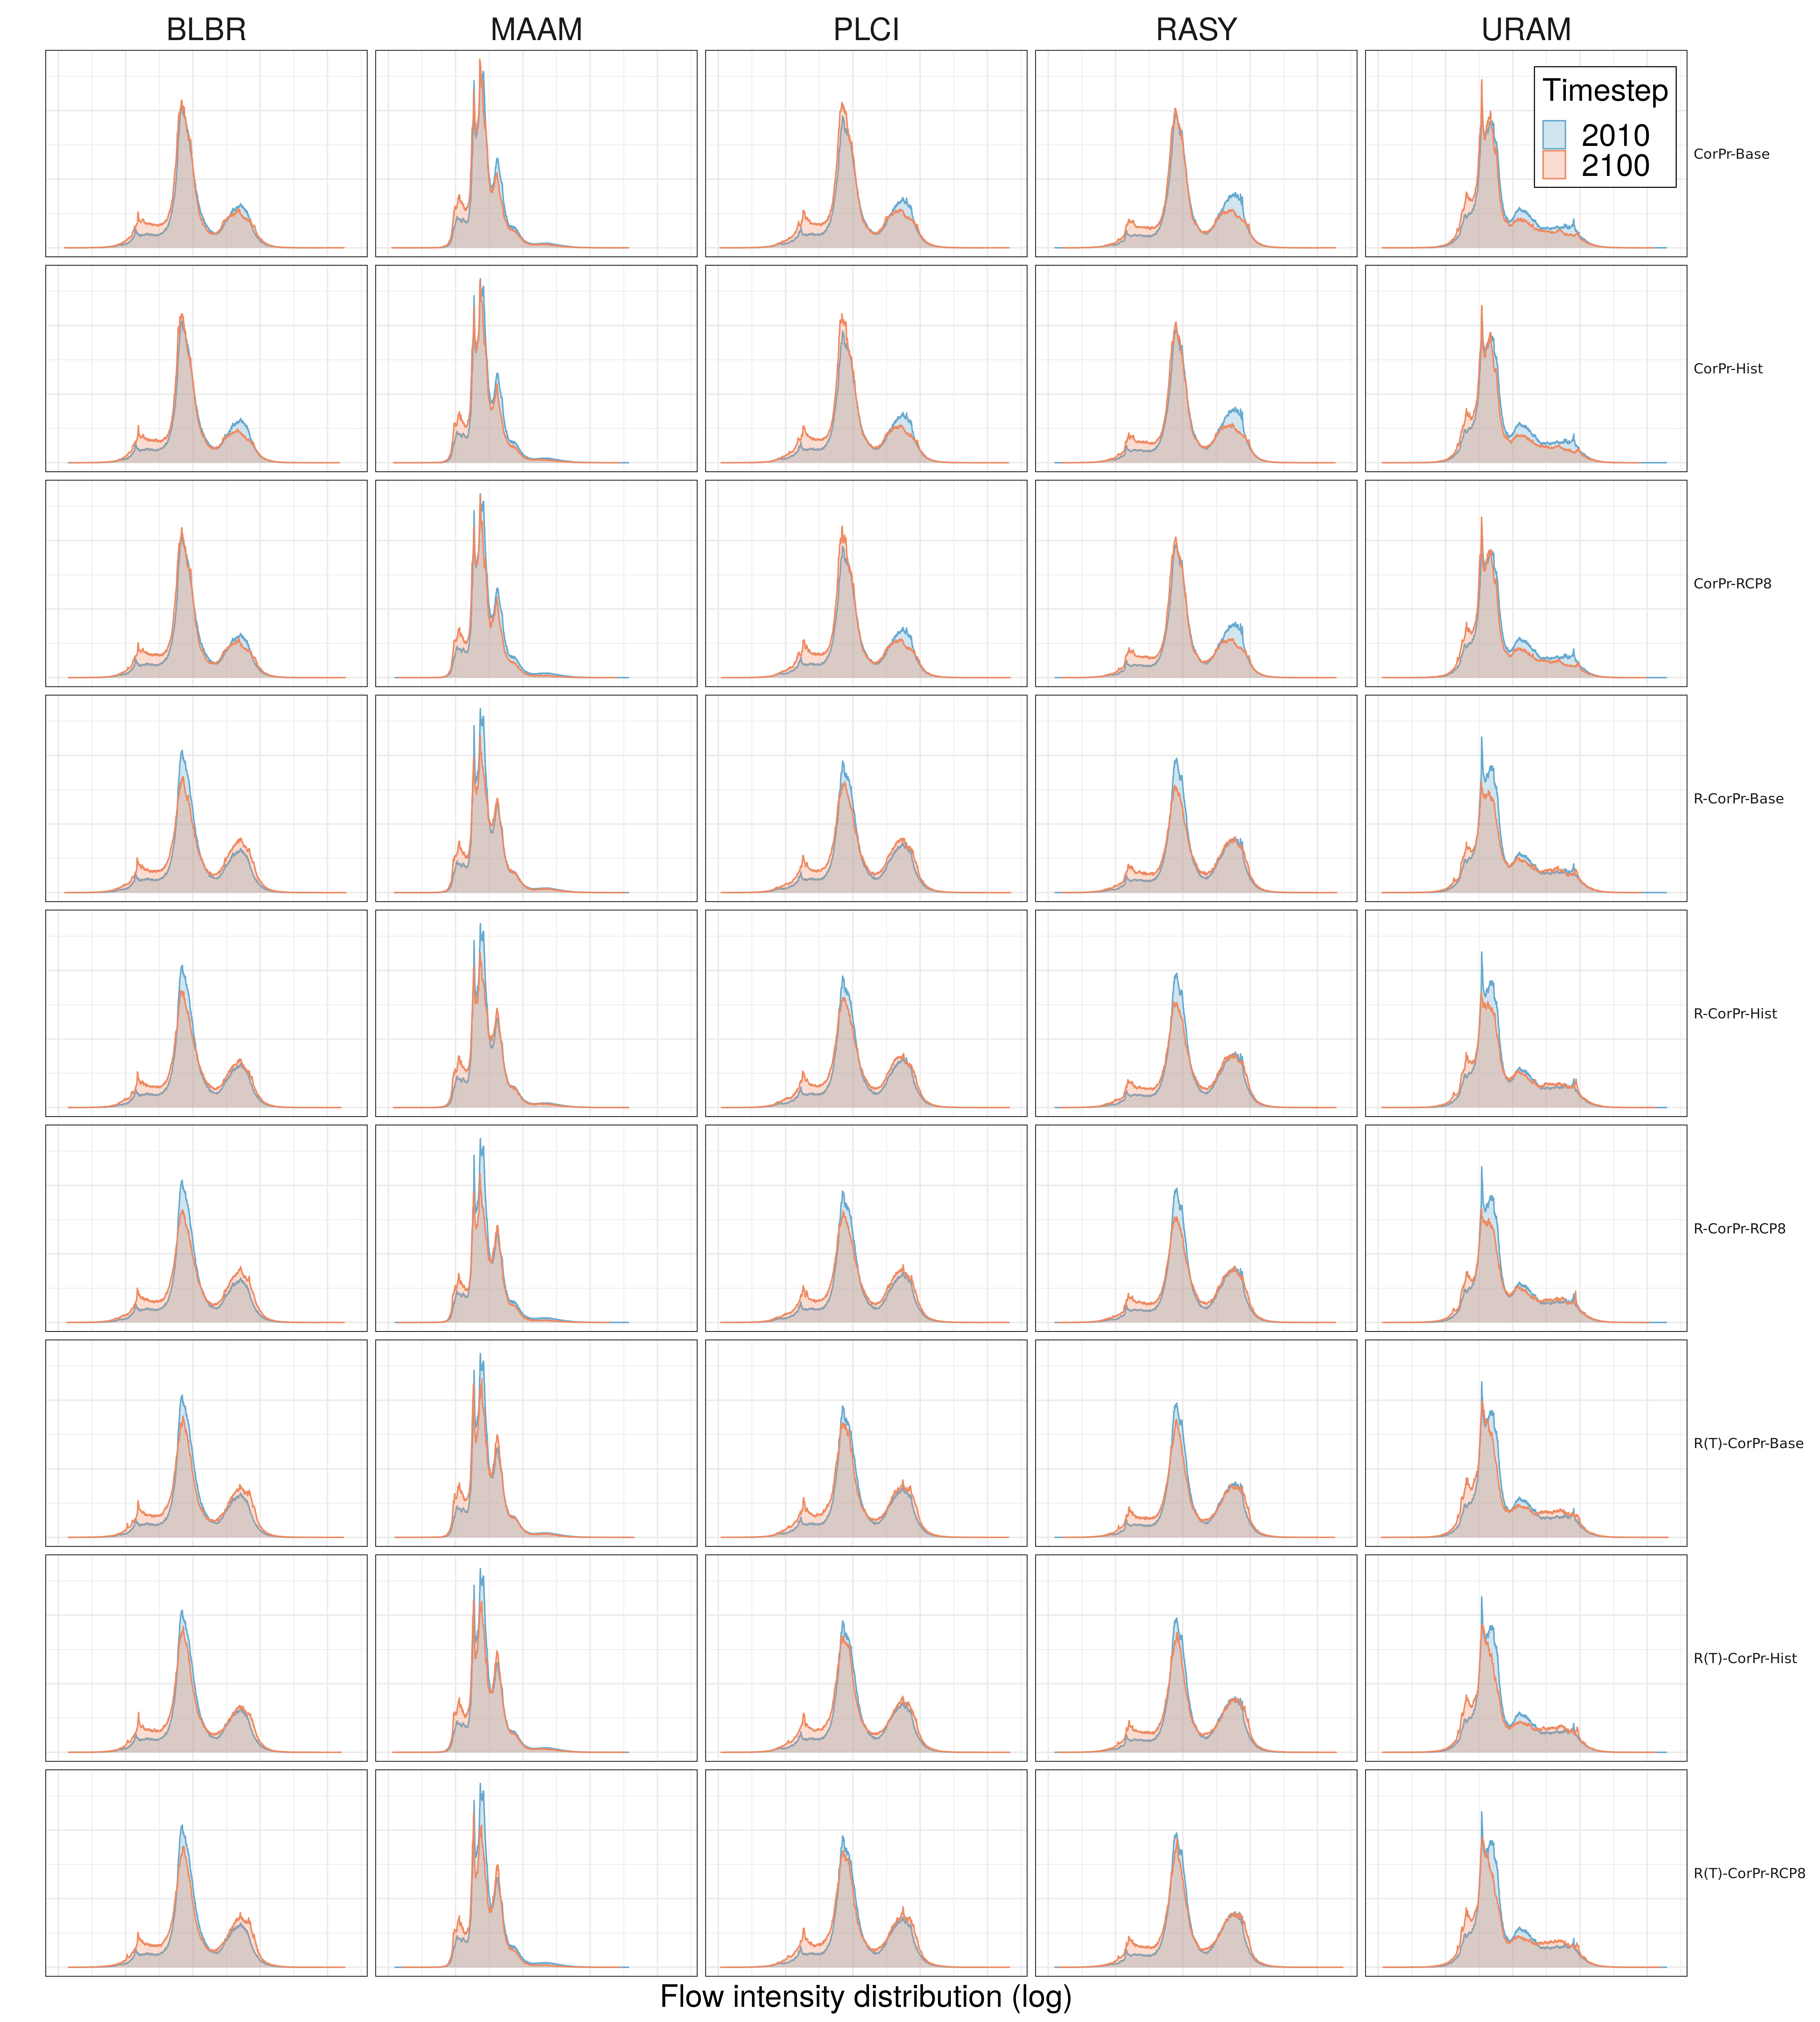
\includegraphics[width=1.3\textwidth]{thesis/figures/hist_chap2.png}
}
 \caption{Histograms of flow values for all species and scenarios, for 2010 (observed) and 2100 (predicted).}
 \label{fig:hist_2}
\end{figure}

%---------------------------------------------------------------------------------------------------------------------------------------------------
% SURF

% Linear
\begin{figure}[h!]
\makebox[\textwidth]{
  \includegraphics[width=1.3\textwidth]{thesis/figures/surf_chap2.png}
}
 \caption{Change in the number of features (in \% of the 2010 flow) identified by the SURF analysis between 2010 (observed) and 2100 (predicted), contrasting BAU scenario with other conservation scenarios - linear graph.}
 \label{fig:surf_linear_2}
\end{figure}

% Radar
\begin{figure}[h!]
\makebox[\textwidth]{
  \includegraphics[width=1.3\textwidth]{thesis/figures/surf_radar_chap2.png}
}
 \caption{Change in the number of features (in \% of the 2010 flow) identified by the SURF analysis between 2010 (observed) and 2100 (predicted), contrasting BAU scenario with other conservation scenarios - radar graph.}
 \label{fig:surf_radar_2}
\end{figure}

\printbibliography[heading=bibintoc, section=2, title={Chapter 2 Bibliography \hspace{1em}}]

\endrefsection

\newpage

%%%%%%%%%%%%%%%%%%%%%%%%%%%%%%%%%%%%%%%%%%%%%%%%%%
%%        General Discussion                     %
%%%%%%%%%%%%%%%%%%%%%%%%%%%%%%%%%%%%%%%%%%%%%%%%%%
% Clearly state the rationale and objectives of the research.
\newcommand*{\SetDiscName}[1]{\renewcommand*{\ETDDiscName}{#1}}%
\newcommand*{\ETDDiscName}{Disc}%

\newcommand{\SetDiscText}[1]{\renewcommand*{\ETDDiscText}{#1}}%
\newcommand*{\ETDDiscText}{Disc text goes here!}%

\newcommand{\Disc}{%
    \begin{simpleenv}{}{}{}{}%
    \pagestyle{plain}%
  \setboolean{SetDSpace}{false}%
    \GoSingle%
    \begin{QZ@Cent}%
          \bfseries{\ETDDiscName}
      \end{QZ@Cent}%
    \vspace*{0.5in}
      \par%
      \GoDouble%
      \setlength{\parskip}{-2em}
      %\chapter*{\ETDDiscName}%
      \phantomsection\section*{}
      \addcontentsline{toc}{extrachapter}{\ETDDiscName}%
      \ETDDiscText%
    \end{simpleenv}%
    \setboolean{SetDSpace}{true}}%
%%%%%%%%%%%%%%%%%%%%%%%%%%%%%%%%%%%%%%%%%%%%%%%%%%%%

% Discussion
%%%%%%%%%%%%%%%%%%%%%%%%%%%%%%%%%%%%%%%%%%%%%%%%%%%%
\SetDiscName{General Discussion}%

\SetDiscText{

The two chapters of this thesis alleviate two limitations to Connectivity Conservation Planning methods identified in the general introduction: the lack of methodological integration between connectivity, land use change and climate change models; and the need for stakeholder inputs in the planning process. \\

In chapter 1, we integrated circuit-theory based connectivity models with a simple land use and scenarios from a climate change model based on habitat suitability for 5 umbrella species. We also presented patterns of land use change in our study region for the 1990-2010 period, and demonstrated that our land use change model captures these general patterns across the landscape. We analysed changes in connectivity under simple land use and climate change scenarios, and showed that different species have different responses, depending on the forest type they depend on, and on whether this forest type is under threat from land use change, climate change or both. The American marten showed the most complex response because it is dependent on coniferous forest, which is the most at risk under both drivers. We also used a pattern-detection method (SURF) to identify pinch-points and salient connectivity flow features. Although the number of features detected is species-specific, we showed a mostly consistent pattern of change over time: reforestation seems to simplify the flows of movement on the landscape. More research to understand the links between flow complexity and SURF measures is needed. \\

Then, in chapter 2, we capitalized on the progress in chapter 1 by including the results of a stakeholder workshop during which we mapped areas of consensus among stakeholders that were deemed important for connectivity in the region. During this participatory process, we also identified key assets (such as the drive and momentum of conservation NGOs in the region) and obstacles (such as the predominance of an agricultural matrix) to connectivity conservation in the region. We derived simple conservation scenarios based on priorities identified during the participatory mapping exercise. We simulated connectivity changes for our five species under these scenarios and made clear the complexity of restoring connectivity to cater to species with different needs while accounting for multiple stakeholder interests. \\

I now address some general limitations that concern both chapters. We argued that using markov-chain monte carlo (MCMC) based modelling for land use change allowed us to take into account the uncertainty of land use change simulations. The principle is to run the model multiple times (iterations), resulting in slightly different simulations every time. This allowed us to see that our model was quite constrained and that over 10 iterations we produced narrow confidence intervals when analysing the resulting connectivity; this was true for both chapters. However, there remains a large amount of uncertainty unaccounted for in the model. STSIM required a large number of parameters (for example, neighboring parameters, see \ref{tab:neigh_rules}) that were chosen and fixed to a certain value. To correctly account for uncertainty in those parameters, we could decide on a distribution for those parameters and draw from this distribution at each iteration. This is possible in STSIM, which allows the user to specify distributions. However this brings its own set of drawbacks. First, in order to get a representative sample from this distribution, more iterations would need to be computed, which would increase computing time. Second, the shape of the distribution for parameters like neighboring rules is not easy to determine a priori. This last point could potentially be alleviated by sampling the distribution from historical land use and land cover change data ; however, the question of how to conduct this sampling appropriately, for instance to account for spatial autocorrelation, is not straightforward. \\

Our approach to modeling functional connectivity was focused on potential functional connectivity (PFC). In both chapters, we use circuit theory to model PFC. A first limitation is that the choice of the methods employed modelling will inevitably influence the way connectivity corridors are designed, and therefore it is important to keep in mind that different methods could lead to different designs. Second, a limitation of PFC modelling is that what the model produces is an informed prediction about potential movement, which is still in need of statistical validation with data derived from movement events observed on the landscape. Therefore, the quality of the data used for parameterization of the resistance surface is extremely important for the accuracy of the results. In addition, circuit theory has been criticized as a PFC approach. \cite{fletcher_spatial_2018} mention a set of issues: first, animals might not move in a way that can realistically be modelled as random walks. It is computationally more expensive than least-cost path analysis - although the recent Julia version of Circuitscape is faster and more efficient than previous iterations of the software \citep{anantharaman_circuitscape_2020}. They also argue that results can be difficult to interpret across large landscapes, given the fact that flow tends to be predicted as being diffuse. Finally, they mention an issue that “has been neglected in the ecological literature but has been repeatedly acknowledged in the network literature.” According to \cite{luxburg_hitting_2014}, on large graphs, the resistance distance  between patches converges on the local properties at a cell level, making the use of random walks less helpful. \\

However, connectivity research can be hopeful in its ability to move beyond those limitations. Resistance-based models have been validated with genetic data \citep{marrotte_landscape_2014} and occurrence data (\cite{gray_landscape_2016}) and movement data \citep{lapoint_animal_2013}. Although genetic data alone cannot be expected to predict demographic connectivity without information on local demographic rates \citep{lowe_what_2010}, it can provide important information on connectivity when combined with other data sources. Connectivity modelling therefore needs to move toward new, integrative, and data-rich approaches. One example is combining multi-scale resistance surfaces from multiple data types, as \cite{zeller_multi-level_2017} did for pumas (\textit{Puma concolor}) in southern California. The role of novel forms of modelling, such as Individual-Based Models (IBMs, a form of Agents-Based Models) is another potential direction for connectivity research: they can add realism to resistance based and circuit theory models and bring attention to mechanisms overlooked by those models, like mortality \citep{day_individual-based_2020}. In all cases, these approaches are data-intensive and seem to point to a need for more data on animal movements. \\

Finally, in both chapters we pointed out the limitations in the way we defined land use change and conservation scenarios. Although the goal was to derive simple and extreme cases to show the range of variations in species’ responses, this method will remain unsatisfactory for stakeholders, until it is inscribed in an interactive process of community-driven scenario building (see discussion at the  end of Chapter 2). Both chapters outline the design principles for a tool that could be used to facilitate this iterative process, by providing information on the consequence of “what if” scenarios on potential functional connectivity. It is important to ask what framework would best allow us to operationalize this tool and allow researchers to provide guidance to stakeholders during a decision making process. In the following, we discuss the importance of the Spatialized SES (SpaSES, \cite{williamson_spatially_2018}), and Ecosystem Services Bright Spots \citep{frei_bright_2018} frameworks to guide the design of connectivity conservation planning tools. \\

Having recognized that conservation tools often fail to consider social factors affecting their implementation, \cite{williamson_spatially_2018} developed the SpaSES framework as a recontextualization of Ostrom’s framework applied to conservation tools. In the original SES framework, SES variables are numerous, and acquiring data on them for decision making at large spatial scales is often impossible. Therefore, \citeauthor{williamson_spatially_2018} bundled them in three categories, forming a three dimensional space across which probability of conservation action can be modelled. First, Ecological Value (EV) describes how important an habitat is for conservation. Then, Social Willingness (SW) and Institutional Capacity (IC) account for social factors. Social willingness variables essentially take stock of the level of social acceptability to conservation, based on theories of individual and collective behavior. Institutional Capacity variables measure governance systems, institutional fit, and factors that influence the capacity of institutions of different types (government, action groups) to reach conservation goals. \citeauthor{williamson_spatially_2018} models probability of connectivity as a function of those three latent variables (EV, SW, IC), for which they suggest a number of proxies that will vary depending on study region and conservation objectives. \\

For our study region, an appropriate measure of EV could be the results of a prioritization of habitat patches based on habitat suitability and connectivity at different scales under land use and climate change, such as in \cite{albert_applying_2017}. But \citeauthor{williamson_spatially_2018} notes that this type of prioritization effects “generally assume that stakeholders are interested in an optimal solution to resource management concerns and pursue those solutions rationally, ” an assumption they argue is not confirmed by SES research. One way to tackle this rational optimization fallacy is to use multi-criteria weightings systems to avoid optimizing with only one outcome in mind. This justifies the need for taking other dimensions of conservation action (SW and IC) into account. Participatory methods such as the one we employed could be an appropriate way of developing measures for these two axes, as stakeholders most likely know what variables would be better representative of each axis. An iterative process of scenario building could be initiated by efforts to define (1) multiple scenarios based on stakeholder’s perceptions of planning priorities, (2) a measure of SW for conservation, partially based on alignment with the different scenarios developed and (3) a measure of stakeholders’s confidence in IC in the region to conduct different conservation plans, and an idea of what the needs are in IC for such plans to succeed. This framework would lead to better estimates of where conservation is both critical and implementable in the region. \\

Workshops might also be a good tool to build up SW and IC themselves and increase the probability of conservation action, which will in a large part depend on the obstacles identified in any workshop. According to our results, the most obvious of these obstacles in our region is the predominance of agricultural land use. The role of the agricultural matrix in fragmented landscapes became under scrutiny when the SLOSS debate in ecology \citep{diamond_island_1975, simberloff_island_1976}, was for a time renewed in the land sparing versus land sharing debate \citep{fischer_land_2014}. The concept at the base of these dichotomies, is that smaller fragments experience higher extinction, and that connectivity can help by restoring immigration between fragments. \cite{perfecto_natures_2019} points out that focusing on connectivity and immigration rates in fragmented landscapes actually “means focusing on the agroecosystems, which in turn means examining what is happening socio-politically in the agricultural matrix” \citep{perfecto_natures_2019}. Both the “single large/several small” and “sharing/sparing” oppositions are now seen as false dichotomies, rendered obsolete by the SES literature. \cite{bennett_changing_2017} agrees and argues that those dichotomies have tended to look at agroecosystems too simply, mostly within the angle of food production. They propose we go beyond those dichotomies by acknowledging the multiple facets of agroecosystems and considering the complexity of the agro-ecological matrix. \\

One way to embrace the complexity of the matrix is to carefully look at the relationship between the structure of a landscape and its impact on connectivity and associated ecosystem functions, such as carbon storage or pollination \citep{mitchell_linking_2013}. Both Models \citep{mitchell_strong_2015} and empirical studies \citep{mitchell_forest_2014} have shown that landscape complexity can modify biodiversity, connectivity and ecosystem service supply. While earlier studies focused on single services, more research is looking into how connectivity of forest fragments impact a wide diversity of services\citep{mitchell_forest_2014}. For example, crop heterogeneity is linked to higher biodiversity \citep{sirami_increasing_2019}. Agricultural matrices with smaller average field sizes tend to be more biodiverse \citep{fahrig_farmlands_2015}. These phenomena have been attributed to an increase in connectivity due to the presence of more semi-natural habitats. These contributions are important and should be considered for land use planning. They are appealing for the design of connectivity conservation tools, because they point out clear management scenarios that could be tested through models, and can make use of the increasing availability of high resolution remotely sensed data. \\

But, as we quoted from \cite{williamson_spatially_2018} above, this view tends to assume that stakeholders want to pursue rational and optimal designs in their approach to conservation. There is a tendency to take a single-faceted approach to the optimisation problem, focusing on the trade-off between food production and the support for biodiversity. An alternative way is through the lens of ecosystem services  \citep{bennett_changing_2017}. Ecosystem services refer to the diversity of benefits that ecosystems provide to, and the many ways in which they support, human systems. Specifically, the concept of “bright spots" has potential for guiding the discussion beyond dichotomies and single faceted approaches, by focusing on multifunctionality in agroecosystems. In a landscape, “bright spots” are areas exceeding expectations for goals, such as agro-ecological multifunctionality, biodiversity, or connectivity \citep{frei_bright_2018}. They show promise as a tool to identify levers of change, and guide stakeholder discussion. Indeed, an approach that focuses on identifying bright spots for the provision of those ecosystem services can be valuable to an interactive process of stakeholder engagement. They offer starting points to work with to design alternative plausible scenarios, which can then feed the reflexion of stakeholders \citep{bernier_modelisation_2013, theau_evaluation_2015}. Bright spots are concrete examples to reason around what bundles of ecosystem services are desirable (elements of SW) for the conservation of ecological connectivity and which types of governance is needed to work toward them (elements of IC). In our study region, this framework is already being tested: \cite{frei_bright_2018} identified bright, dark and average spots within Montérégie for both landscape multifunctionality and avian biodiversity. They showed important spatial properties of bright spots, for instance that they were “neither spatially congruent nor in conflict”. Connectivity could be fully integrated with this approach in two ways: first, it would be interesting to see if current bright spots are congruent with connectivity, in order to assess the mismatch between connectivity and other bundles of ecosystem services. One example is that of bee diversity which was found to be higher in connected habitats in Montérégie \citep{martins_complementary_2018}. Second, areas that are prioritized as important for connectivity under models such as the ones we developed in chapter 1 could be used in the identification of bright spots. \\

\citeauthor{frei_bright_2018} also pointed out a range of challenges for the identification of bright spots, the development of multicriteria measures being one of them. Connectivity measures are already being developed with  multifunctionality in mind. For instance, \cite{rayfield_priorisation_2018}, assessed whether certain habitat networks in the Montérégie would be more resilient to future change using several multi-scale metrics of connectivity. Another example is \cite{fletcher_towards_2019} who developed an unifying model for connectivity that takes into account multiple aspects of animal mobility. Connectivity is therefore a field that fits in the multicriteria framework of bright spots, as it itself moves in this direction. Bright spots show promise for being integrated in more complex connectivity conservation planning tools. Finally, bright spots are intuitive, being based on statistical deviation from a given distribution and are therefore always relative to the context in which they are implemented. They are suited to the type of participatory framework we implemented in chapter 2: bundles of ecosystem services that are important to stakeholders can be identified and bright spots can be discussed, all in the iterative participatory setting we detailed above. \\

\vspace{3em}

\subsection*{\textit{Conclusion \\ \vspace{2em}}}
\addcontentsline{toc}{chapter}{Conclusion}

The integration of models of multiple drivers of changes in ecological connectivity with stakeholder inputs into connectivity models will contribute to the design of better connectivity conservation planning tools. In this thesis, we contributed some design elements for those tools, such as a methodology to account for uncertainty and an approach to integrating the different  priorities among local stakeholders. Future research will need to engage in an iterative process of regional stakeholder engagement, possibly including a scenario building exercise. This process will be all the more successful if it is made within a coherent framework that addresses the social-ecological complexity of fragmented landscapes, such as SpaSES and Bright spots. These frameworks will guide discussion and facilitate the visualization of positive alternative scenarios to business as usual. \\
}%

\Disc%

% Appendix
%\ETDAppendix{Chapter I Supplementary Material}{
%% !TEX root = ./thesis.tex

\chapter*{\textbf{Appendix 1: Chapters Supplementary Material \\ \hspace{1em}}}
\addcontentsline{toc}{chapter}{Appendix 1: Chapters Supplementary Material}
\addcontentsline{toc}{section}{Chapter I Supplementary Material}

\setcounter{chapter}{3}
\setcounter{table}{0}
\setcounter{figure}{0}

%---------------------------------------------------------------------------------------------------------------------------------------------------
% METHODS CHAP1

% %\begin{landscape}
% \begin{longtable}[c]{|p{5cm}|p{11cm}|}
% %\centering
% \caption{Description of the 5 umbrella species (adapted from \cite{rayfield_priorisation_2018}).}
% \label{tab:species} \\
% %\begin{tabular}{|p{5cm}|p{10cm}|}
% \hline
% \hline
% \textbf{Species} & \textbf{Description} \\ \hline
% Northern short-tailed Shrew \newline \textit{Blarina brevicauda} & Abundant small fossorial mammal. This highly active species can live in a diversity of habitats (grasslands, old fields, marshy areas, gardens, and some developed areas) but is mainly found in deciduous and mixed old forests with thick understories that provide good cover for hiding from predators. It feeds primarily on earthworms found in areas with moist soils. It has a high reproductive rate and is generally a poor disperser although it can cross gaps of 50-100m. \\ \hline
% American marten \newline \textit{Martes americana} & Small vagile carnivorous predator. Found in core areas of dense (\textgreater{}60\% cover) and old (\textgreater{}70 yr) coniferous or mixed forests with complex vertical and horizontal structure. It requires large home ranges (above hundreds of ha). It generally avoids large openings and clearings (above a few hundred meters wide) but crosses roads and frozen rivers easily. Deep persistent snow pack is a habitat critical element as it excludes predators (Canis latrans) and competitors (Martes pennanti) and provides good hunting conditions. This forest specialist is particularly sensitive to human activities. Juveniles are able to cover tens of kilometers when dispersing, more than what would be expected from body mass-based estimates. Trapped for its fur, this species has patrimonial and economical importance. \\ \hline
% Red-Backed Salamander \newline \textit{Plethodon cinereus} & Terrestrial salamander. This sedentary and territorial forest-dwelling species lives under the leaf litter or coarse woody debris in mature and moist deciduous and mixed forests. It is a poor disperser that uses tens of square meters as a home range and rarely ventures more than 50 m in open fields. Roads and edges (up to 20-30 m) have a negative effect on populations’ densities and reduce individual movements. \\ \hline
% Wood Frog \newline \textit{Rana sylvatica} & Forest-specialist amphibian. This species prefers mixed and coniferous stands with closed canopy (\textgreater 40\%) and moist soil covered with woody debris (for egg deposition) but can adapt to other closed habitats. Both aquatic (palustrine, fish-free wetlands, not open and permanent ones) and terrestrial habitats are essential, and distance between both should not exceed ca. 600 m. It is sensitive to forest edge (25-35 m), gaps, high intensity agriculture, human developments and recent clearcuts that can act as barriers to movement. This poor disperser is particularly sensitive to roads and habitat loss (fidelity to the first breeding pond). \\ \hline
% Black Bear \newline \textit{Ursus americanus} & Large opportunistic omnivorous mammal. This species likes deciduous and mixed mature forest with dense cover interspersed with small clearings and early-successional stages of forest that are rich in berry production (depends on main soil surface deposit). It uses broad territories (tens to hundreds of square km) to follow the fruiting season by going upslope with the season. It is an effective seed disperser because it can travel long distances (up to 390 km), in particular male juveniles. It clearly avoids human activity (up to 5 km) and roads (up to 800 m), in particular highways, and is likely to take a detour instead of crossing a 60 m gap. \\
% \hline
% \hline
% %\end{tabular}
% \end{longtable}
% %\end{landscape}

%---------------------------------------------------------------------------------------------------------------------------------------------------
% RF

% RF variables

\begin{table}[h!]
\centering
\caption{Description and data sources for all variables used in the Random Forest - Cellular Automata model.}
\label{tab:variables}
\begin{tabular}{lll}
\hline
\textbf{Variable} & \textbf{Format} & \textbf{Source}  \\ 
\hline
Distance from urban land & \multirow{3}{*}{Raster} & \multirow{2}{*}{Generated from land cover data} \\ \cline{1-1}
Size of forest patch &  &  \\ \cline{1-1} \cline{3-3} 
Elevation &  & \begin{tabular}[c]{@{}l@{}}SRTM 30m from Google \\ Earth Engine data library\end{tabular} \\ \hline
Population change & \multirow{2}{*}{\begin{tabular}[c]{@{}l@{}}Tabular data joined to vector \\ data and rasterized\end{tabular}} & \multirow{2}{*}{\begin{tabular}[c]{@{}l@{}}Canadian Census for \\ 1991, 2001 and 2011\end{tabular}} \\ \cline{1-1}
Income &  &  \\ \hline
Road network & Vector data (rasterized) & Adresses Québec \\ 
\hline
\end{tabular}
\end{table}

%---------------------------------------------------------------------------------------------------------------------------------------------------
% STSIM

% Neighborhood rules

\begin{table}[h!]
\centering
\caption[Rules for the transitions in the land use change model]{Rules for the transitions in the land use change model. The transition is only allowed if the Proportion of the Pixel counted is reached in the Neighborhood.}
\label{tab:neigh_rules}
\begin{tabular}{llcc}
\hline
\textbf{Transition} & \textbf{Pixel counted} & \textbf{Neighborhood (m)} & \textbf{Minimum Proportion} \\ \hline
Urbanization & Urban & 500 & 0.7 \\
Agricultural Expansion & Agriculture & 250 & 0.9 \\
Reforestation & Forest (any type) & 250 & 0.9 \\
Forest Internals & Forest (specific type) & 225 & 0.15 \\ \hline
\end{tabular}
\end{table}

%---------------------------------------------------------------------------------------------------------------------------------------------------
% Connectivity analyses

% Habitat suitability 

\begin{table}[h!]
\centering
\caption[Rules for the suitability analysis of forest pixels]{Rules for the suitability analysis of forest pixels. For each species, forest pixels are classified into suitability values based on forest types and age.}
\label{tab:suit_pixls}
\begin{tabular}{lccccccccc}
\textbf{} & \multicolumn{3}{c}{\textbf{Deciduous}} & \multicolumn{3}{c}{\textbf{Mixed}} & \multicolumn{3}{c}{\textbf{Coniferous}} \\ \hline
\textbf{Species} & \textbf{Young} & \textbf{Medium} & \textbf{Old} & \textbf{Young} & \textbf{Medium} & \textbf{Old} & \textbf{Young} & \textbf{Medium} & \textbf{Old} \\ \hline
\textit{\begin{tabular}[c]{@{}l@{}}Blarina \\ brevicauda\end{tabular}} & 0 & 0.5 & 1 & 0 & 0.5 & 1 & 0 & 0 & 0 \\ \hline
\textit{\begin{tabular}[c]{@{}l@{}}Martes \\ americana\end{tabular}} & 0 & 0 & 0 & 0 & 1 & 1 & 1 & 1 & 1 \\ \hline
\textit{\begin{tabular}[c]{@{}l@{}}Plethodon \\ cinereus\end{tabular}} & 1 & 1 & 1 & 1 & 0.5 & 1 & 0 & 0 & 0 \\ \hline
\textit{\begin{tabular}[c]{@{}l@{}}Rana \\ sylvatica\end{tabular}} & 1 & 1 & 1 & 1 & 1 & 1 & 1 & 1 & 1 \\ \hline
\textit{\begin{tabular}[c]{@{}l@{}}Ursus\\ americanus\end{tabular}} & 1 & 1 & 1 & 0.5 & 0.5 & 0.5 & 1 & 1 & 1 \\ \hline
\end{tabular}
\end{table}

% Reclassification into resistance

\begin{table}[h!]
\centering
\caption[Rules for the reclassification into resistance of non-forest pixels]{Rules for the reclassification into resistance of non-forest pixels. For all species, pixels of different land uses are classified into the same resistance values.}
\label{tab:key_non_forest}
\begin{tabular}{lcccccc}
\hline
\textbf{Species} & \textbf{Urban land} & \textbf{Roads} & \textbf{Agricultural land} & \textbf{Wetlands} & \textbf{Water} & \textbf{Other} \\ \hline 
\textit{\begin{tabular}[c]{@{}l@{}}Blarina \\ brevicauda\end{tabular}} 	&  32 & 32 &	8    & 8 & 16 & 8\\ \hline
\textit{\begin{tabular}[c]{@{}l@{}}Martes \\ americana\end{tabular}} 	&  32 & 32 &	16  & 8 &	 16 & 8\\ \hline
\textit{\begin{tabular}[c]{@{}l@{}}Plethodon \\ cinereus\end{tabular}} 	&  32 & 32 &	8    & 8 & 32 & 8	\\ \hline
\textit{\begin{tabular}[c]{@{}l@{}}Rana \\ sylvatica\end{tabular}} 			&  32 & 32 &	8    & 2 & 8   &	 8	\\ \hline
\textit{\begin{tabular}[c]{@{}l@{}}Ursus\\ americanus\end{tabular}} 		&  32 & 32 &	16  & 2 &	 16 & 8\\ \hline
\end{tabular}
\end{table}

% Minimum patch

\begin{table}[h!]
\centering
\caption[Minimum patch size rules for the suitability analysis of forest patches]{Minimum patch size rules for the suitability analysis of forest patches. A patch of forest is only deemed suitable if its size is above the minimum size.}
\label{tab:patch_size}
\begin{tabular}{lc}
\hline
\textbf{Species} & \textbf{Minimum patch size} (hectares) \\ \hline 
\textit{\begin{tabular}[c]{@{}l@{}}Blarina brevicauda\end{tabular}} 	&  1		\\ \hline
\textit{\begin{tabular}[c]{@{}l@{}}Martes americana\end{tabular}} 	&  150		\\ \hline
\textit{\begin{tabular}[c]{@{}l@{}}Plethodon cinereus\end{tabular}} 	&  1		\\ \hline
\textit{\begin{tabular}[c]{@{}l@{}}Rana sylvatica\end{tabular}} 			&  1		\\ \hline
\textit{\begin{tabular}[c]{@{}l@{}}Ursus americanus\end{tabular}} 		&  1200		\\ \hline
\end{tabular}
\end{table}

% Key patches type

\begin{table}[h!]
\centering
\caption[Rules for the reclassification into resistance of forest patches]{Rules for the reclassification into resistance of forest patches. For each species, forest patches are classified into different resistance values based on whether they are considered suitable habitat, too small or non-habitat. For a patch to be considered habitat, the majority of its pixels mush have a suitability value of 1 (see table \ref{tab:suit_pixls}) and its size must be above the minimum size for the species (see table \ref{tab:patch_size}.}
\label{tab:hab_or_not}
\begin{tabular}{lccc}
\hline
\textbf{Species} & \textbf{Habitat patch} & \textbf{Habitat patch - too small} & \textbf{Non-habitat patch} \\ \hline 
\textit{\begin{tabular}[c]{@{}l@{}}Blarina \\ brevicauda\end{tabular}} 	&	1	&	2	&	4	\\ \hline
\textit{\begin{tabular}[c]{@{}l@{}}Martes \\ americana\end{tabular}} 	&  1	&	4	&	8	\\ \hline
\textit{\begin{tabular}[c]{@{}l@{}}Plethodon \\ cinereus\end{tabular}} 	&  1	&	2	&	4	\\ \hline
\textit{\begin{tabular}[c]{@{}l@{}}Rana \\ sylvatica\end{tabular}} 			&  1	&	2	&	4	\\ \hline
\textit{\begin{tabular}[c]{@{}l@{}}Ursus\\ americanus\end{tabular}} 		&  1	&	4	&	16	\\ \hline
\end{tabular}
\end{table}

% SURF

\begin{table}[h!]
\centering
\caption[SURF analysis parameters.]{Parameters for the SURF (Speeded-up Robust Features) analysis (Feature detection analysis). Parameters were chosen arbitrarily (see methods).}
\label{tab:surf}
\begin{tabular}{lc}
\hline
\hline
Parameter & Value \\ \hline
Hessian threshold & 7000 \\
Number of octaves & 1 \\
Number of octave layers & 2 \\ \hline
\end{tabular}
\end{table}

%---------------------------------------------------------------------------------------------------------------------------------------------------
% RESULTS CHAP1

% Clustering

% VALUES

% \begin{figure}[h!]
% \centering
%  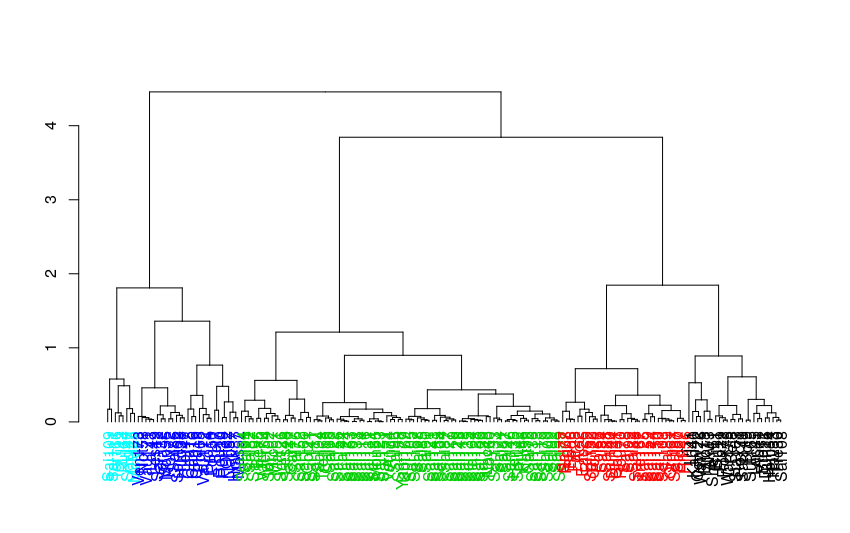
\includegraphics[width=\textwidth]{thesis/figures/clustering_values.png}
%  \caption{Results of Ward clustering for land use for municipalities (cut at 5 groups).}
%  \label{fig:clustervals}
% \end{figure}
% 
% % TRANSITIONS
% \begin{figure}[h!]
%     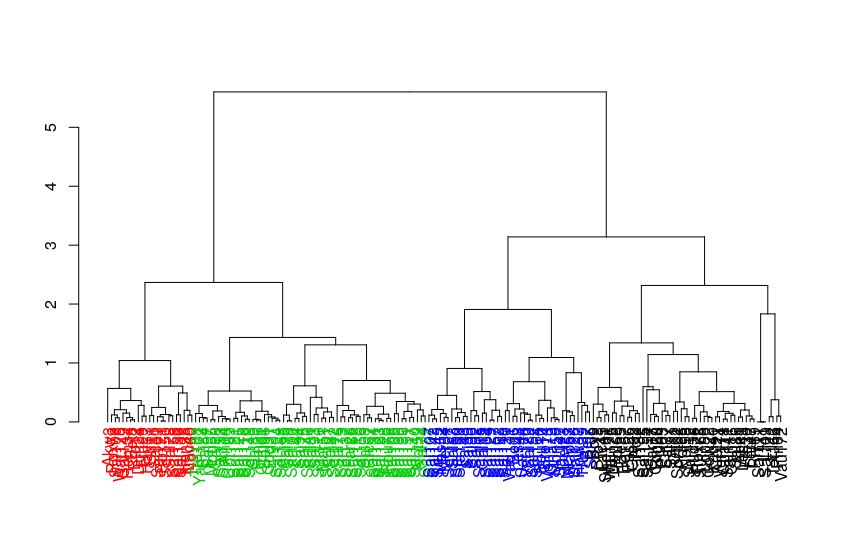
\includegraphics[width=\textwidth]{thesis/figures/clustering_trans.png}
%   \caption{Results of Ward clustering for transition data for municipalities (cut at 4 groups).}
%   \label{fig:clustertrans}
% \end{figure}

%---------------------------------------------------------------------------------------------------------------------------------------------------
% ROC Curves

% Agex

% \begin{figure}[h!]
% \makebox[\textwidth]{
%   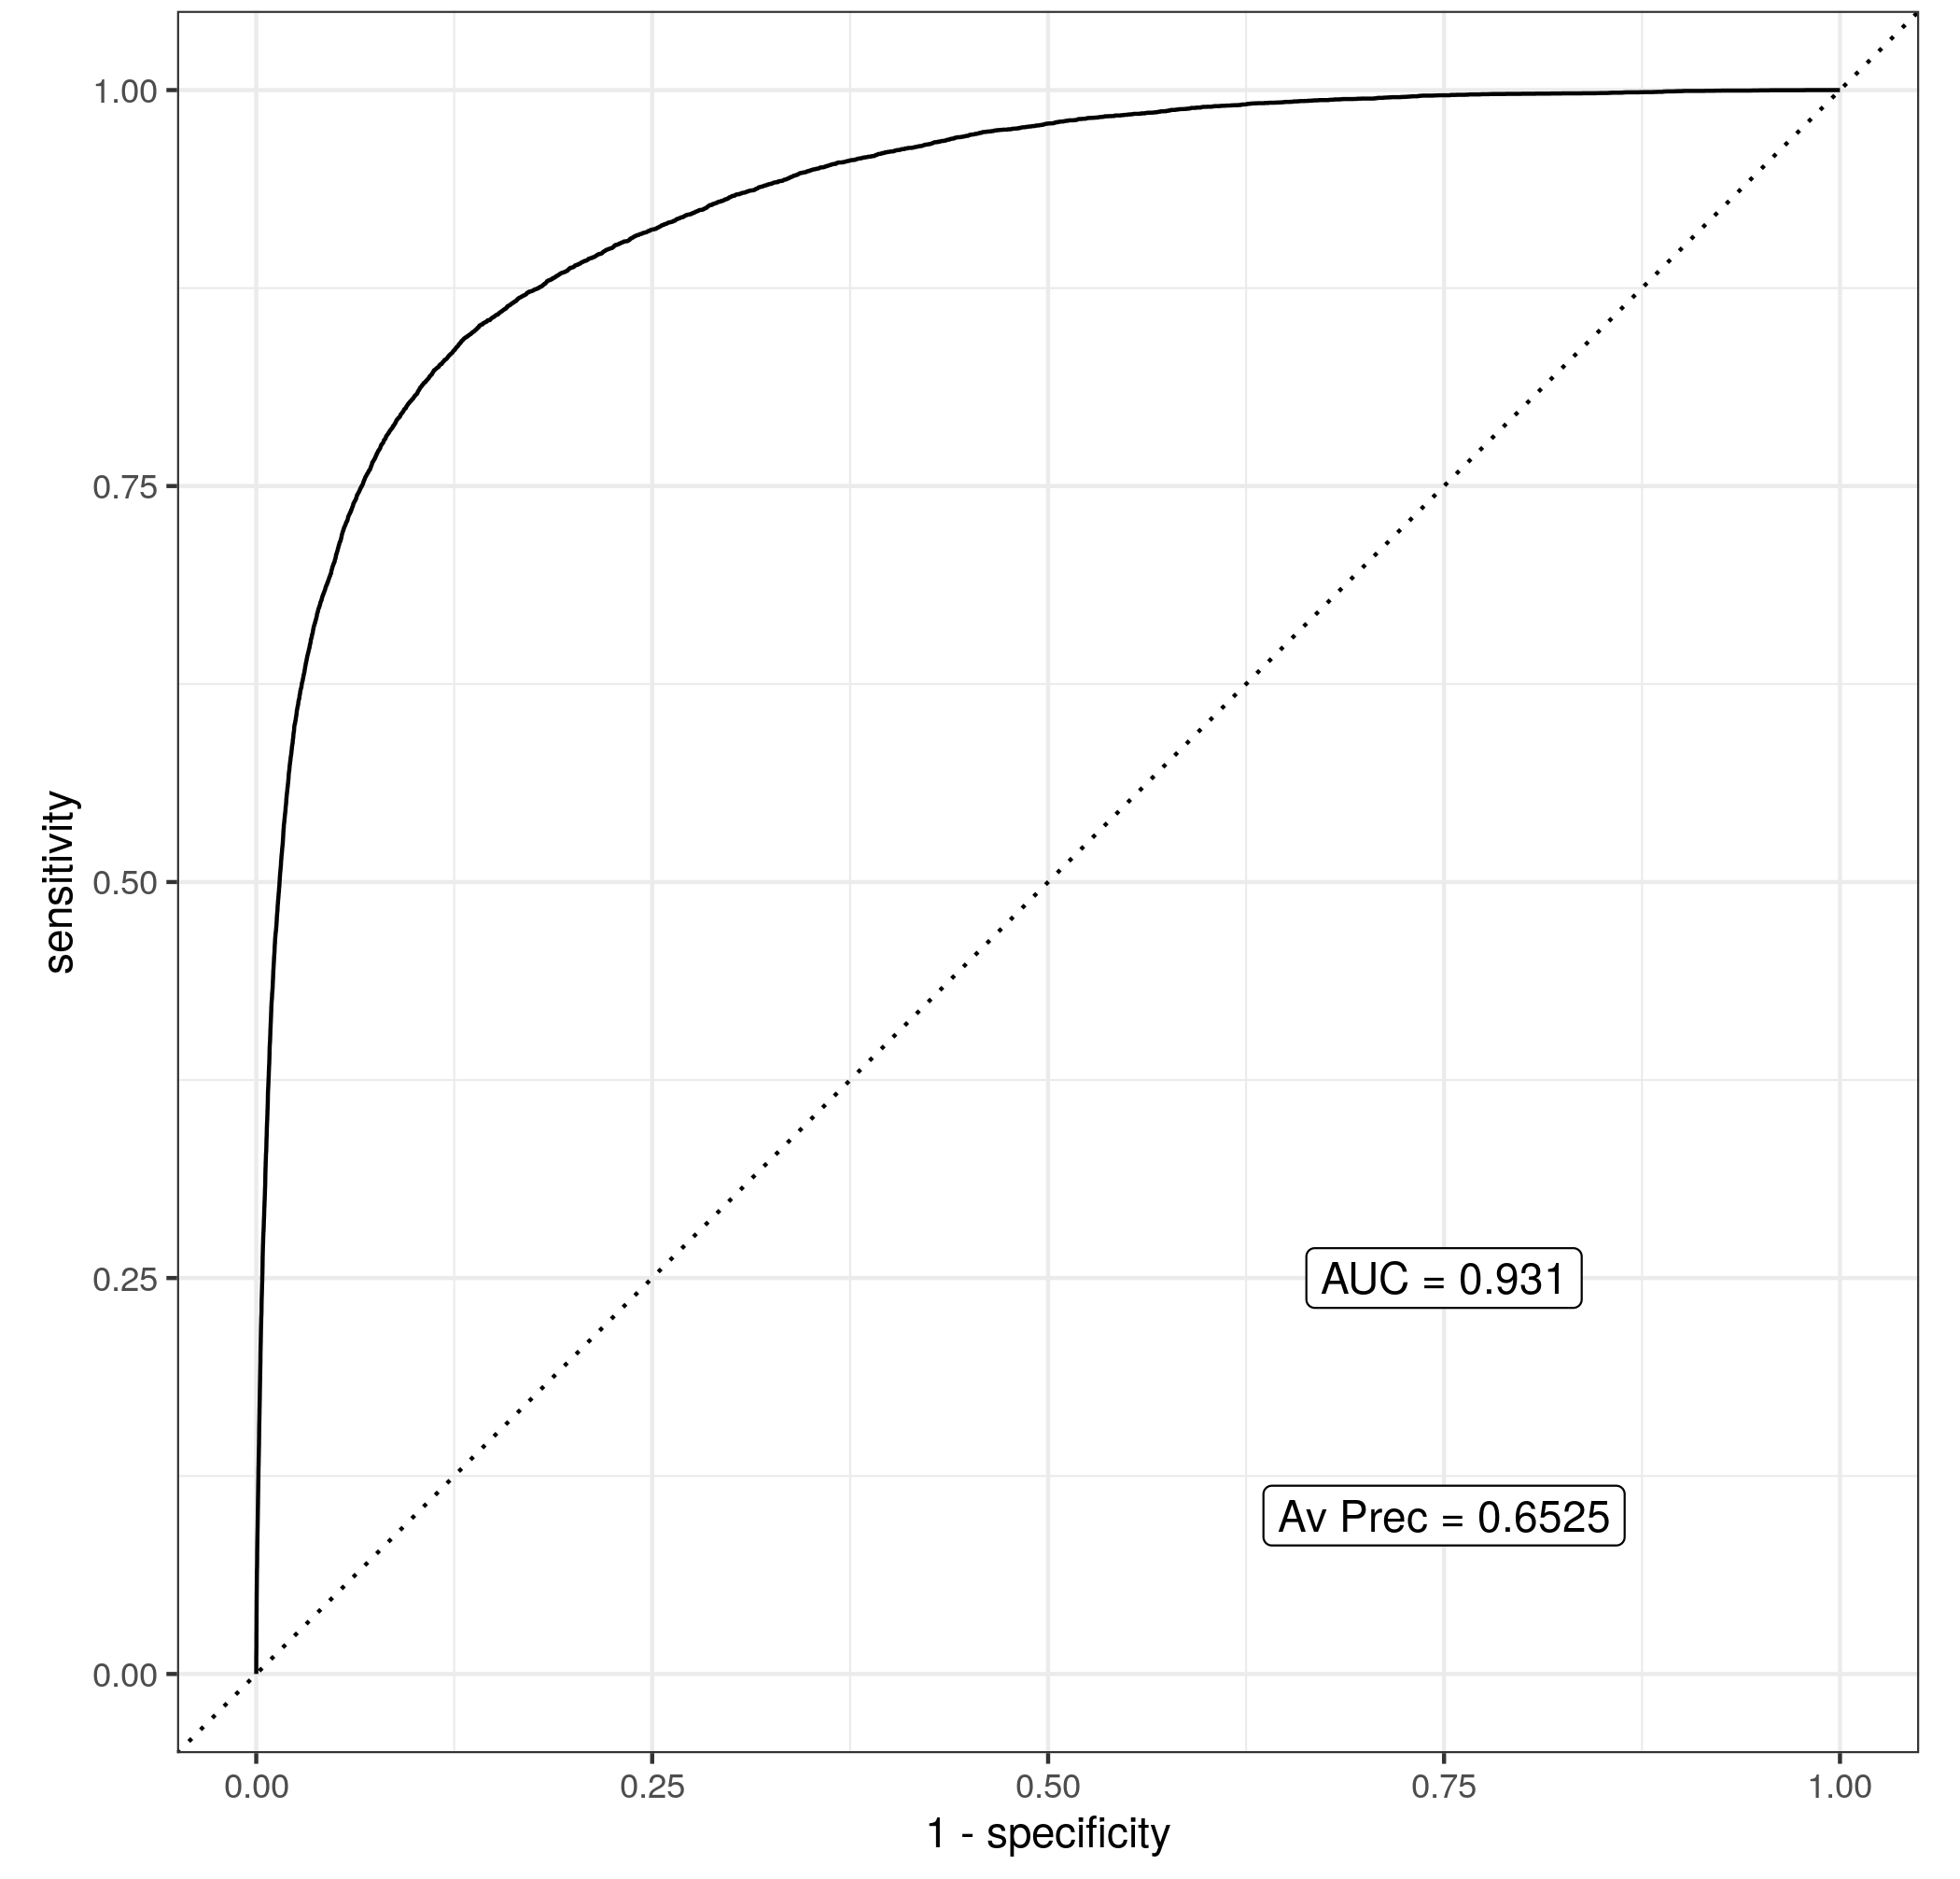
\includegraphics[width=\textwidth]{thesis/figures/rf_ratio_2_agex_roc.png}
% }
%  \caption{ROC Curve for Agricultural Expansion.}
%  \label{fig:roc_agex}
% \end{figure}
% 
% % Urb
% 
% \begin{figure}[h!]
% \makebox[\textwidth]{
%   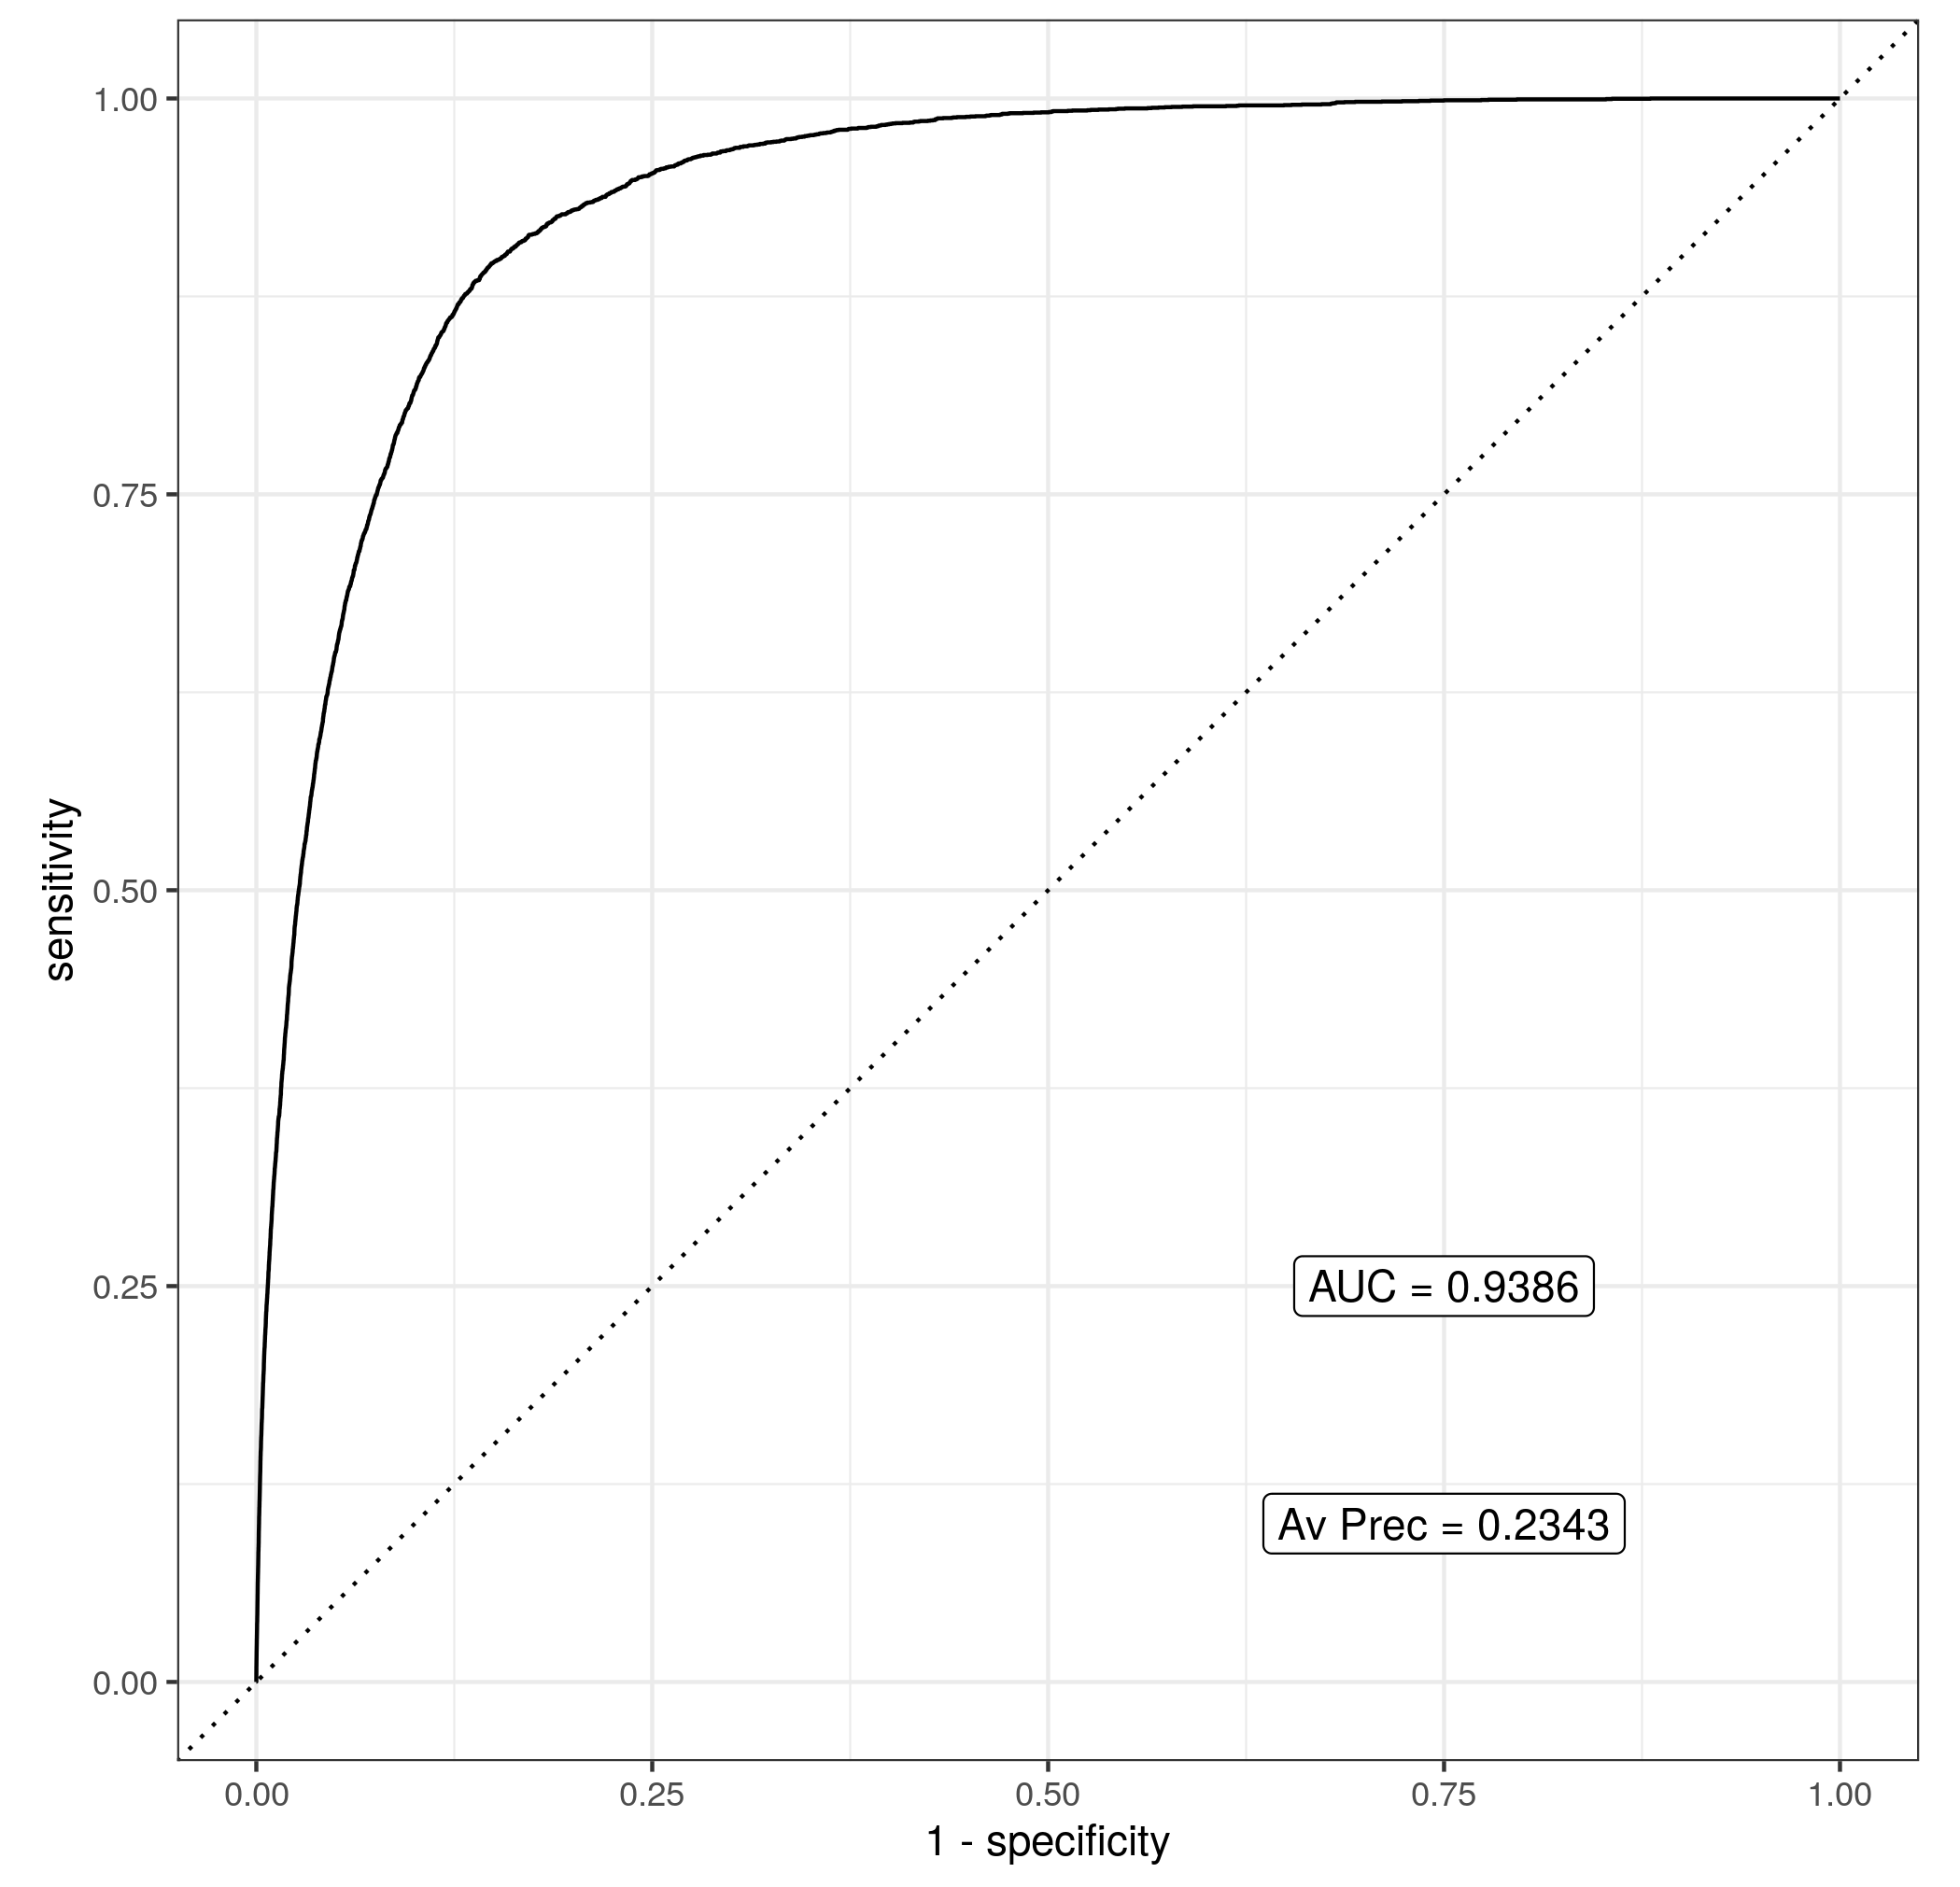
\includegraphics[width=\textwidth]{thesis/figures/rf_ratio_2_urb_roc.png}
% }
%  \caption{ROC Curve for Urbanisation.}
%  \label{fig:roc_urb}
% \end{figure}

%  Resample, figure and table

\begin{figure}[h!]
\makebox[\textwidth]{
  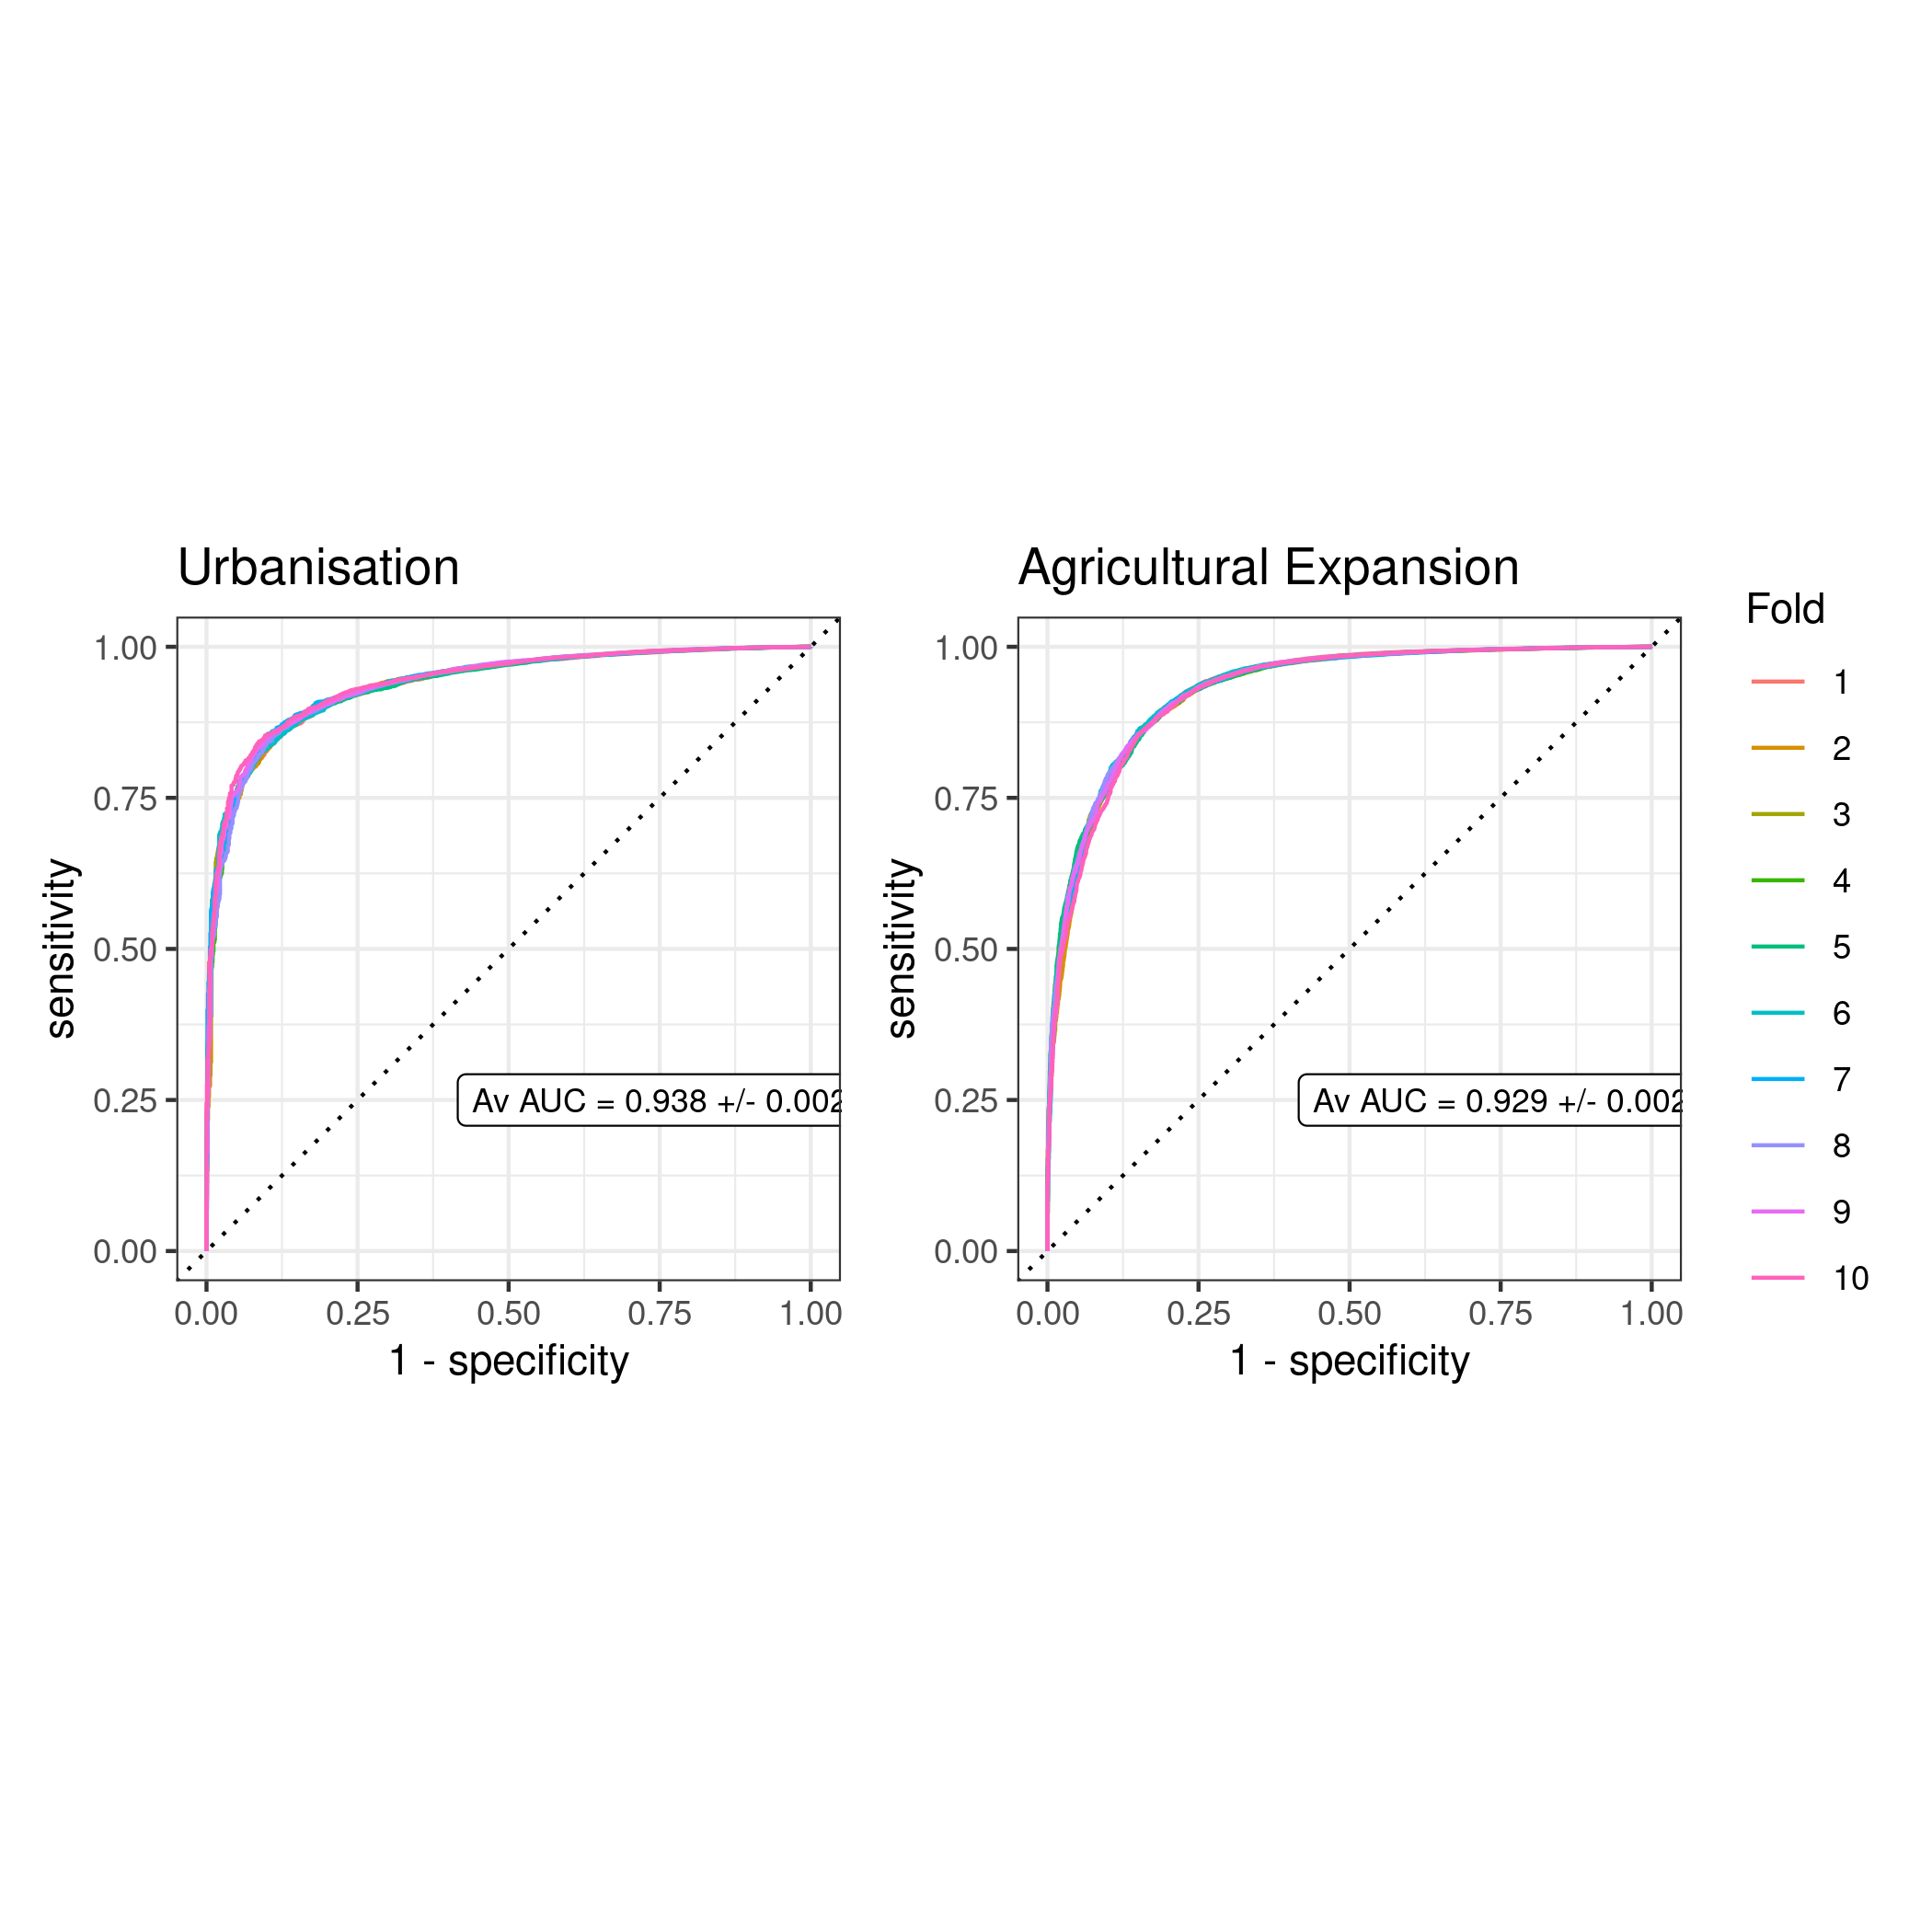
\includegraphics[width=1.3\textwidth]{thesis/figures/double_roc_resample.png}
}
 \caption[ROC Curves for re-samples for Agricultural Expansion and Urbanisation]{ROC curves (Receiver Operating Characteristic) for the results of the Random Forest models for both Agricultural Expansion and Urbanisation. Results are given for the 10 Fold CCV (Classic Cross-Validation). The average AUC (Area Under Curve) for each model (+/- standard deviation) is also given.}
 \label{fig:roc_rs}
\end{figure}

%---------------------------------------------------------------------------------------------------------------------------------------------------
% Maps compare

\begin{figure}[h!]
\makebox[\textwidth]{
  \includegraphics[width=1.3\textwidth]{thesis/figures/scenario_39_compare.png}
}
 \caption[Map of Montérégie at the beginning of the BAU scenario in 2010, and at the end in 2100 (under baseline climate scenario)]{Map of Montérégie at the beginning of the BAU (Business as Usual) scenario in 2010, and at the end of the simulation in 2100 (under baseline climate scenario)}
 \label{fig:BAU_compare}
\end{figure}

\begin{figure}[h!]
\makebox[\textwidth]{
  \includegraphics[width=1.3\textwidth]{thesis/figures/scenario_42_compare.png}
}
 \caption[Map of Montérégie at the beginning of the Reforestation scenario in 2010, and at the end in 2100 (under baseline climate scenario)]{Map of Montérégie at the beginning of the Reforestation scenario in 2010, and at the end of the simulation in 2100 (under baseline climate scenario).}
 \label{fig:Ref_compare}
\end{figure}

\newpage

%---------------------------------------------------------------------------------------------------------------------------------------------------

\chapter*{\textbf{Chapter II Supplementary Material \\ \hspace{1em}}}
\addcontentsline{toc}{section}{Chapter II Supplementary Material}

%---------------------------------------------------------------------------------------------------------------------------------------------------
% METHODS/results CHAP2

% Workshop tables

\begin{table}[h!]
\centering
\caption[Summary table of the community workshop: opportunities and challenges - non spatial elements (French)]{Summary table of the community workshop: opportunities and challenges identified by workshop participants. All non spatial elements (i.e. not mapped by participants) are listed.}
\label{tab:opp_chall_ns}
\begin{tabular}{m{0.15\textwidth}lm{0.5\textwidth}l}
\hline
\textbf{Table} &
  \textbf{\begin{tabular}[c]{@{}l@{}}Atout/Contrainte \\ (Opportunity/Challenge)\end{tabular}} &
  \textbf{\begin{tabular}[c]{@{}l@{}}Contenu\\ (Content)\end{tabular}} &
  \textbf{Score} \\ \hline
\multirow{5}{*}{Centre} &
  \multirow{3}{*}{Atouts} &
  Présence d'organisme environnementaux &
  8.00 \\ \cline{3-4} 
                       &                              & Basses terres: lien prioritaire l’échelle nationale & 4.00  \\ \cline{3-4} 
                       &                              & Programme ALUS                                      & 1.00  \\ \cline{2-4} 
                       & \multirow{2}{*}{Contraintes} & CPTAQ                                               & 18.00 \\ \cline{3-4} 
                       &                              & Besoin de rentabilité des entreprises agricoles     & 5.00  \\ \hline
\multirow{3}{*}{Est}   & Atouts                       & Vocation forestiere existante                       & 8.00  \\ \cline{2-4} 
                       & \multirow{2}{*}{Contraintes} & Tenure privée des terres                            & 2.00  \\ \cline{3-4} 
                       &                              & Plusieurs territoires couverts                      & 1.00  \\ \hline
\multirow{5}{*}{Nord} &
  \multirow{2}{*}{Atouts} &
  Réglementation favorable maintien couvert bois et corridor métropolitain &
  16.20 \\ \cline{3-4} 
                       &                              & PRMHH                                               & 10.80 \\ \cline{2-4} 
                       & \multirow{3}{*}{Contraintes} & Usage agricole prédominant                          & 44.33 \\ \cline{3-4} 
                       &                              & Compréhension et participation citoyenne            & 14.40 \\ \cline{3-4} 
                       &                              & Coûts pour faire de la connectivité                 & 10.80 \\ \hline
\multirow{6}{*}{Ouest} & \multirow{2}{*}{Atouts}      & Routes cours d'eau                                  & 3.00  \\ \cline{3-4} 
                       &                              & Presence de sols pauvre                             & 3.00  \\ \cline{2-4} 
                       & \multirow{4}{*}{Contraintes} & Les réalités économiques                            & 50.00 \\ \cline{3-4} 
                       &                              & Terres privées                                      & 12.00 \\ \cline{3-4} 
                       &                              & LPTAA                                               & 7.20  \\ \cline{3-4} 
                       &                              & Le monde politique                                  & 4.00  \\ \hline
\multirow{6}{*}{Montérégie} &
  \multirow{4}{*}{Atouts} &
  Milieu agricole: potentiel de faire des corridors si un levier est trouvé &
  12.60 \\ \cline{3-4} 
                       &                              & Présence d'acteurs locaux et éducation              & 8.00  \\ \cline{3-4} 
                       &                              & PRMHH                                               & 3.00  \\ \cline{3-4} 
                       &                              & Permettre l'aménagement forestier                   & 3.00  \\ \cline{2-4} 
                       & \multirow{2}{*}{Contraintes} & Routes et autoroutes                                & 4.00  \\ \cline{3-4} 
                       &                              & Terres privées, présence prédominantes              & 3.00  \\ \hline
\end{tabular}
\end{table}

% Opportunity /challenges

\begin{table}[]
\centering
\caption[Summary table of the community workshop: opportunities and challenges - spatial elements (French)]{Summary table of the community workshop: opportunities and challenges identified by workshop participants. All spatial elements (i.e. mapped by participants) are listed.}
\label{tab:opp_chall_s}
\begin{tabular}{m{0.15\textwidth}lm{0.5\textwidth}l}
\hline
\textbf{Table} &
  \textbf{\begin{tabular}[c]{@{}l@{}}Atout/Contrainte \\ (Opportunity/Challenge)\end{tabular}} &
  \textbf{\begin{tabular}[c]{@{}l@{}}Contenu\\ (Content)\end{tabular}} &
  \textbf{Score} \\ \hline
\multirow{5}{*}{Centre} & Atouts                       & Leaders politiques positifs                                  & 33.33          \\ \cline{2-4} 
                        & Les deux                     & Propriétés protégées                                         & 26.67          \\ \cline{2-4} 
                        & \multirow{3}{*}{Contraintes} & Pressions urbaines                                           & 42.86          \\ \cline{3-4} 
                        &                              & Manque d'adhésion des agriculteurs                           & 39.29          \\ \cline{3-4} 
                        &                              & Pressions agricoles                                          & 16.20          \\ \hline
\multirow{5}{*}{Est}          & Atouts                       & Mobilisation projet corridor bleu vert fondation séthy                         & 18.00 \\ \cline{2-4} 
                        & \multirow{4}{*}{Contraintes} & Autoroute 10                                                 & 26.67          \\ \cline{3-4} 
                        &                              & Pressions villegiatives                                      & 22.2           \\ \cline{3-4} 
                        &                              & Fragmentation des habitats liées au dev                      & 18.00          \\ \cline{3-4} 
                        &                              & Activites agricoles intensives                               & 16.2           \\ \hline
\multirow{4}{*}{Nord}         & \multirow{2}{*}{Atouts}      & Municipalite pro-protection des monteregiennes ex. st bruno mont saint hilaire & 8.00  \\ \cline{3-4} 
                        &                              & Comité municipal travail MRC MDY                             & 1.00           \\ \cline{2-4} 
                        & \multirow{2}{*}{Contraintes} & Autoroute 10 20 30 et autres                                 & 1.00           \\ \cline{3-4} 
                        &                              & Gestion de l'application des bandes riveraines               & 1.00           \\ \hline
\multirow{6}{*}{Ouest}  & \multirow{4}{*}{Atouts}      & Proximité des milieux                                        & 24.00          \\ \cline{3-4} 
                        &                              & Article 50.3 du règlement des exploitations agricoles        & 19.20          \\ \cline{3-4} 
                        &                              & Mobilisation des acteurs du milieux                          & 12.00          \\ \cline{3-4} 
                        &                              & Bande riveraine potentielle                                  & 10.00          \\ \cline{2-4} 
                        & \multirow{2}{*}{Contraintes} & Canal beauharnois isole                                      & 24.00          \\ \cline{3-4} 
                        &                              & Réticences de certains producteurs                           & 10.00          \\ \hline
\multirow{5}{*}{Montérégie 1} & \multirow{3}{*}{Atouts}      & Réseaux de sites avec couvert forestier                                        & 14.4  \\ \cline{3-4} 
                        &                              & Grande volonté d'action locale pour créer de la connectivité & 12.60          \\ \cline{3-4} 
                        &                              & Rétrécissement du fleuve                                     & 7.20           \\ \cline{2-4} 
                              & \multirow{2}{*}{Contraintes} & Agriculture intensive compenser la production                                  & 16.20 \\ \cline{3-4} 
                        &                              & Développement urbain                                         & 12.00          \\ \hline
\multirow{5}{*}{Montérégie 2} & \multirow{2}{*}{Atouts}      & Mobilisation sociale organisme conservation sensibilisation                    & 12.00 \\ \cline{3-4} 
                        &                              & Usage des sols favorable                                     & 10.00          \\ \cline{2-4} 
                        & \multirow{3}{*}{Contraintes} & Prix des terres agricoles                                    & 12.00          \\ \cline{3-4} 
                        &                              & Étalement urbain deuxième couronne                           & 10.00          \\ \cline{3-4} 
                        &                              & Pole logistique de transport                                 & 10.00          \\ \hline
\end{tabular}
\end{table}

\begin{table}[h!]
\centering
\caption[Administrative districts (MRCs) covered by each table in the workshop]{Breakdown of the administrative districts (MRCs, Municipalité Regionales de Comté) covered by each table in the workshop.}
\label{tab:workshoptables}
\begin{tabular}{ll}
\hline
\textbf{Table} & \textbf{MRCs} \\ \hline
Ouest (West) & Vaudreuil, Haut SL, Beauharnois \\
Centre (Center) & Jardins, Haut Richelieu, Rouville, Roussillon \\
Nord (North) & \begin{tabular}[c]{@{}l@{}}Longueuil, Marguerite d'Youville, Vallée du richelieu, \\ Pierre de Saurel, Les Maskoutains\end{tabular} \\
Est & Brome-Missisquoi, Haute Yamaska, Acton \\
Transversal (x2) & Toute la Montérégie (All of  Montérégie)\\ \hline
\end{tabular}
\end{table}

%---------------------------------------------------------------------------------------------------------------------------------------------------
% Maps compare

\begin{figure}[h!]
\makebox[\textwidth]{
  \includegraphics[width=1.3\textwidth]{thesis/figures/scenario_45_compare.png}
}
  \caption[Map of Montérégie at the beginning of the Corridor protection scenario in 2010, and at the end in 2100 (under baseline climate scenario)]{Map of Montérégie at the beginning of the Corridor protection scenario in 2010, and at the end of the simulation in 2100 (under baseline climate scenario).}
 \label{fig:Corr_compare}
\end{figure}

\begin{figure}[h!]
\makebox[\textwidth]{
  \includegraphics[width=1.3\textwidth]{thesis/figures/scenario_48_compare.png}
}
  \caption[Map of Montérégie at the beginning of the Corridor protection + Reforestation scenario in 2010, and at the end in 2100 (under baseline climate scenario)]{Map of Montérégie at the beginning of the Corridor protection + Reforestation scenario in 2010, and at the end of the simulation in 2100 (under baseline climate scenario).}
 \label{fig:	CorrRef_compare}
\end{figure}

\begin{figure}[h!]
\makebox[\textwidth]{
  \includegraphics[width=1.3\textwidth]{thesis/figures/scenario_51_compare.png}
}
  \caption[Map of Montérégie at the beginning of the Corridor protection + Targeted Reforestation scenario in 2010, and at the end in 2100 (under baseline climate scenario)]{Map of Montérégie at the beginning of the Corridor protection + Targeted Reforestation scenario in 2010, and at the end of the simulation in 2100 (under baseline climate scenario).}
 \label{fig:	CorrRefT_compare}
\end{figure}

%---------------------------------------------------------------------------------------------------------------------------------------------------
% Flow

% Radar All
\begin{figure}[h!]
\makebox[\textwidth]{
  \includegraphics[width=1.3\textwidth]{thesis/figures/radar_ggradar_both.png}
}
  \caption[Radar graph of change in mean flow (decrease in \% of the baseline 2010 flow) between 2010 (observed) and 2100 (predicted), comparing all scenarios]{Radar graph of change in mean flow (decrease in \% of the baseline 2010 flow) between 2010 (observed) and 2100 (predicted). This compares all scenarios, for all 5 species. Note that the line color represent species and that each side of the graph is a different scenario.}
 \label{fig:flow_radar_both}
\end{figure}
%}
% !TEX root = ./thesis.tex

\chapter*{\textbf{Appendix 1: Chapters Supplementary Material \\ \hspace{1em}}}
\addcontentsline{toc}{chapter}{Appendix 1: Chapters Supplementary Material}
\addcontentsline{toc}{section}{Chapter I Supplementary Material}

\setcounter{chapter}{3}
\setcounter{table}{0}
\setcounter{figure}{0}

%---------------------------------------------------------------------------------------------------------------------------------------------------
% METHODS CHAP1

% %\begin{landscape}
% \begin{longtable}[c]{|p{5cm}|p{11cm}|}
% %\centering
% \caption{Description of the 5 umbrella species (adapted from \cite{rayfield_priorisation_2018}).}
% \label{tab:species} \\
% %\begin{tabular}{|p{5cm}|p{10cm}|}
% \hline
% \hline
% \textbf{Species} & \textbf{Description} \\ \hline
% Northern short-tailed Shrew \newline \textit{Blarina brevicauda} & Abundant small fossorial mammal. This highly active species can live in a diversity of habitats (grasslands, old fields, marshy areas, gardens, and some developed areas) but is mainly found in deciduous and mixed old forests with thick understories that provide good cover for hiding from predators. It feeds primarily on earthworms found in areas with moist soils. It has a high reproductive rate and is generally a poor disperser although it can cross gaps of 50-100m. \\ \hline
% American marten \newline \textit{Martes americana} & Small vagile carnivorous predator. Found in core areas of dense (\textgreater{}60\% cover) and old (\textgreater{}70 yr) coniferous or mixed forests with complex vertical and horizontal structure. It requires large home ranges (above hundreds of ha). It generally avoids large openings and clearings (above a few hundred meters wide) but crosses roads and frozen rivers easily. Deep persistent snow pack is a habitat critical element as it excludes predators (Canis latrans) and competitors (Martes pennanti) and provides good hunting conditions. This forest specialist is particularly sensitive to human activities. Juveniles are able to cover tens of kilometers when dispersing, more than what would be expected from body mass-based estimates. Trapped for its fur, this species has patrimonial and economical importance. \\ \hline
% Red-Backed Salamander \newline \textit{Plethodon cinereus} & Terrestrial salamander. This sedentary and territorial forest-dwelling species lives under the leaf litter or coarse woody debris in mature and moist deciduous and mixed forests. It is a poor disperser that uses tens of square meters as a home range and rarely ventures more than 50 m in open fields. Roads and edges (up to 20-30 m) have a negative effect on populations’ densities and reduce individual movements. \\ \hline
% Wood Frog \newline \textit{Rana sylvatica} & Forest-specialist amphibian. This species prefers mixed and coniferous stands with closed canopy (\textgreater 40\%) and moist soil covered with woody debris (for egg deposition) but can adapt to other closed habitats. Both aquatic (palustrine, fish-free wetlands, not open and permanent ones) and terrestrial habitats are essential, and distance between both should not exceed ca. 600 m. It is sensitive to forest edge (25-35 m), gaps, high intensity agriculture, human developments and recent clearcuts that can act as barriers to movement. This poor disperser is particularly sensitive to roads and habitat loss (fidelity to the first breeding pond). \\ \hline
% Black Bear \newline \textit{Ursus americanus} & Large opportunistic omnivorous mammal. This species likes deciduous and mixed mature forest with dense cover interspersed with small clearings and early-successional stages of forest that are rich in berry production (depends on main soil surface deposit). It uses broad territories (tens to hundreds of square km) to follow the fruiting season by going upslope with the season. It is an effective seed disperser because it can travel long distances (up to 390 km), in particular male juveniles. It clearly avoids human activity (up to 5 km) and roads (up to 800 m), in particular highways, and is likely to take a detour instead of crossing a 60 m gap. \\
% \hline
% \hline
% %\end{tabular}
% \end{longtable}
% %\end{landscape}

%---------------------------------------------------------------------------------------------------------------------------------------------------
% RF

% RF variables

\begin{table}[h!]
\centering
\caption{Description and data sources for all variables used in the Random Forest - Cellular Automata model.}
\label{tab:variables}
\begin{tabular}{lll}
\hline
\textbf{Variable} & \textbf{Format} & \textbf{Source}  \\ 
\hline
Distance from urban land & \multirow{3}{*}{Raster} & \multirow{2}{*}{Generated from land cover data} \\ \cline{1-1}
Size of forest patch &  &  \\ \cline{1-1} \cline{3-3} 
Elevation &  & \begin{tabular}[c]{@{}l@{}}SRTM 30m from Google \\ Earth Engine data library\end{tabular} \\ \hline
Population change & \multirow{2}{*}{\begin{tabular}[c]{@{}l@{}}Tabular data joined to vector \\ data and rasterized\end{tabular}} & \multirow{2}{*}{\begin{tabular}[c]{@{}l@{}}Canadian Census for \\ 1991, 2001 and 2011\end{tabular}} \\ \cline{1-1}
Income &  &  \\ \hline
Road network & Vector data (rasterized) & Adresses Québec \\ 
\hline
\end{tabular}
\end{table}

%---------------------------------------------------------------------------------------------------------------------------------------------------
% STSIM

% Neighborhood rules

\begin{table}[h!]
\centering
\caption[Rules for the transitions in the land use change model]{Rules for the transitions in the land use change model. The transition is only allowed if the Proportion of the Pixel counted is reached in the Neighborhood.}
\label{tab:neigh_rules}
\begin{tabular}{llcc}
\hline
\textbf{Transition} & \textbf{Pixel counted} & \textbf{Neighborhood (m)} & \textbf{Minimum Proportion} \\ \hline
Urbanization & Urban & 500 & 0.7 \\
Agricultural Expansion & Agriculture & 250 & 0.9 \\
Reforestation & Forest (any type) & 250 & 0.9 \\
Forest Internals & Forest (specific type) & 225 & 0.15 \\ \hline
\end{tabular}
\end{table}

%---------------------------------------------------------------------------------------------------------------------------------------------------
% Connectivity analyses

% Habitat suitability 

\begin{table}[h!]
\centering
\caption[Rules for the suitability analysis of forest pixels]{Rules for the suitability analysis of forest pixels. For each species, forest pixels are classified into suitability values based on forest types and age.}
\label{tab:suit_pixls}
\begin{tabular}{lccccccccc}
\textbf{} & \multicolumn{3}{c}{\textbf{Deciduous}} & \multicolumn{3}{c}{\textbf{Mixed}} & \multicolumn{3}{c}{\textbf{Coniferous}} \\ \hline
\textbf{Species} & \textbf{Young} & \textbf{Medium} & \textbf{Old} & \textbf{Young} & \textbf{Medium} & \textbf{Old} & \textbf{Young} & \textbf{Medium} & \textbf{Old} \\ \hline
\textit{\begin{tabular}[c]{@{}l@{}}Blarina \\ brevicauda\end{tabular}} & 0 & 0.5 & 1 & 0 & 0.5 & 1 & 0 & 0 & 0 \\ \hline
\textit{\begin{tabular}[c]{@{}l@{}}Martes \\ americana\end{tabular}} & 0 & 0 & 0 & 0 & 1 & 1 & 1 & 1 & 1 \\ \hline
\textit{\begin{tabular}[c]{@{}l@{}}Plethodon \\ cinereus\end{tabular}} & 1 & 1 & 1 & 1 & 0.5 & 1 & 0 & 0 & 0 \\ \hline
\textit{\begin{tabular}[c]{@{}l@{}}Rana \\ sylvatica\end{tabular}} & 1 & 1 & 1 & 1 & 1 & 1 & 1 & 1 & 1 \\ \hline
\textit{\begin{tabular}[c]{@{}l@{}}Ursus\\ americanus\end{tabular}} & 1 & 1 & 1 & 0.5 & 0.5 & 0.5 & 1 & 1 & 1 \\ \hline
\end{tabular}
\end{table}

% Reclassification into resistance

\begin{table}[h!]
\centering
\caption[Rules for the reclassification into resistance of non-forest pixels]{Rules for the reclassification into resistance of non-forest pixels. For all species, pixels of different land uses are classified into the same resistance values.}
\label{tab:key_non_forest}
\begin{tabular}{lcccccc}
\hline
\textbf{Species} & \textbf{Urban land} & \textbf{Roads} & \textbf{Agricultural land} & \textbf{Wetlands} & \textbf{Water} & \textbf{Other} \\ \hline 
\textit{\begin{tabular}[c]{@{}l@{}}Blarina \\ brevicauda\end{tabular}} 	&  32 & 32 &	8    & 8 & 16 & 8\\ \hline
\textit{\begin{tabular}[c]{@{}l@{}}Martes \\ americana\end{tabular}} 	&  32 & 32 &	16  & 8 &	 16 & 8\\ \hline
\textit{\begin{tabular}[c]{@{}l@{}}Plethodon \\ cinereus\end{tabular}} 	&  32 & 32 &	8    & 8 & 32 & 8	\\ \hline
\textit{\begin{tabular}[c]{@{}l@{}}Rana \\ sylvatica\end{tabular}} 			&  32 & 32 &	8    & 2 & 8   &	 8	\\ \hline
\textit{\begin{tabular}[c]{@{}l@{}}Ursus\\ americanus\end{tabular}} 		&  32 & 32 &	16  & 2 &	 16 & 8\\ \hline
\end{tabular}
\end{table}

% Minimum patch

\begin{table}[h!]
\centering
\caption[Minimum patch size rules for the suitability analysis of forest patches]{Minimum patch size rules for the suitability analysis of forest patches. A patch of forest is only deemed suitable if its size is above the minimum size.}
\label{tab:patch_size}
\begin{tabular}{lc}
\hline
\textbf{Species} & \textbf{Minimum patch size} (hectares) \\ \hline 
\textit{\begin{tabular}[c]{@{}l@{}}Blarina brevicauda\end{tabular}} 	&  1		\\ \hline
\textit{\begin{tabular}[c]{@{}l@{}}Martes americana\end{tabular}} 	&  150		\\ \hline
\textit{\begin{tabular}[c]{@{}l@{}}Plethodon cinereus\end{tabular}} 	&  1		\\ \hline
\textit{\begin{tabular}[c]{@{}l@{}}Rana sylvatica\end{tabular}} 			&  1		\\ \hline
\textit{\begin{tabular}[c]{@{}l@{}}Ursus americanus\end{tabular}} 		&  1200		\\ \hline
\end{tabular}
\end{table}

% Key patches type

\begin{table}[h!]
\centering
\caption[Rules for the reclassification into resistance of forest patches]{Rules for the reclassification into resistance of forest patches. For each species, forest patches are classified into different resistance values based on whether they are considered suitable habitat, too small or non-habitat. For a patch to be considered habitat, the majority of its pixels mush have a suitability value of 1 (see table \ref{tab:suit_pixls}) and its size must be above the minimum size for the species (see table \ref{tab:patch_size}.}
\label{tab:hab_or_not}
\begin{tabular}{lccc}
\hline
\textbf{Species} & \textbf{Habitat patch} & \textbf{Habitat patch - too small} & \textbf{Non-habitat patch} \\ \hline 
\textit{\begin{tabular}[c]{@{}l@{}}Blarina \\ brevicauda\end{tabular}} 	&	1	&	2	&	4	\\ \hline
\textit{\begin{tabular}[c]{@{}l@{}}Martes \\ americana\end{tabular}} 	&  1	&	4	&	8	\\ \hline
\textit{\begin{tabular}[c]{@{}l@{}}Plethodon \\ cinereus\end{tabular}} 	&  1	&	2	&	4	\\ \hline
\textit{\begin{tabular}[c]{@{}l@{}}Rana \\ sylvatica\end{tabular}} 			&  1	&	2	&	4	\\ \hline
\textit{\begin{tabular}[c]{@{}l@{}}Ursus\\ americanus\end{tabular}} 		&  1	&	4	&	16	\\ \hline
\end{tabular}
\end{table}

% SURF

\begin{table}[h!]
\centering
\caption[SURF analysis parameters.]{Parameters for the SURF (Speeded-up Robust Features) analysis (Feature detection analysis). Parameters were chosen arbitrarily (see methods).}
\label{tab:surf}
\begin{tabular}{lc}
\hline
\hline
Parameter & Value \\ \hline
Hessian threshold & 7000 \\
Number of octaves & 1 \\
Number of octave layers & 2 \\ \hline
\end{tabular}
\end{table}

%---------------------------------------------------------------------------------------------------------------------------------------------------
% RESULTS CHAP1

% Clustering

% VALUES

% \begin{figure}[h!]
% \centering
%  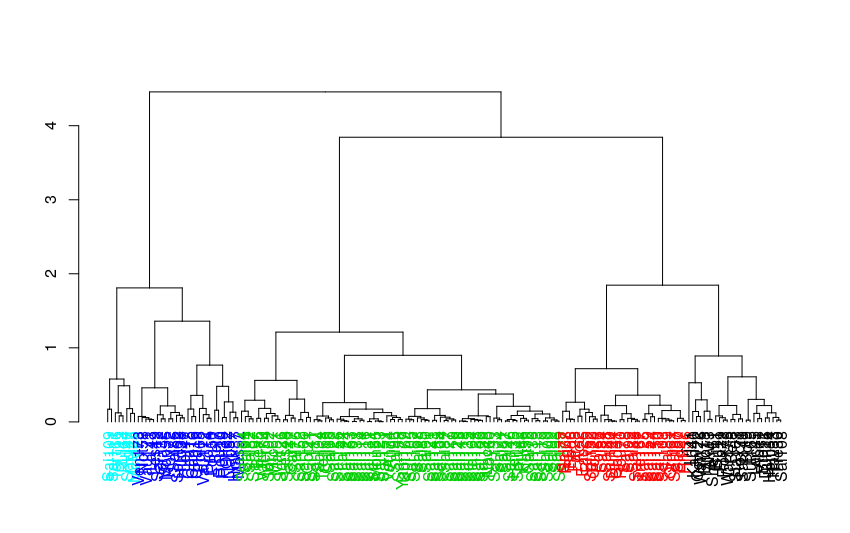
\includegraphics[width=\textwidth]{thesis/figures/clustering_values.png}
%  \caption{Results of Ward clustering for land use for municipalities (cut at 5 groups).}
%  \label{fig:clustervals}
% \end{figure}
% 
% % TRANSITIONS
% \begin{figure}[h!]
%     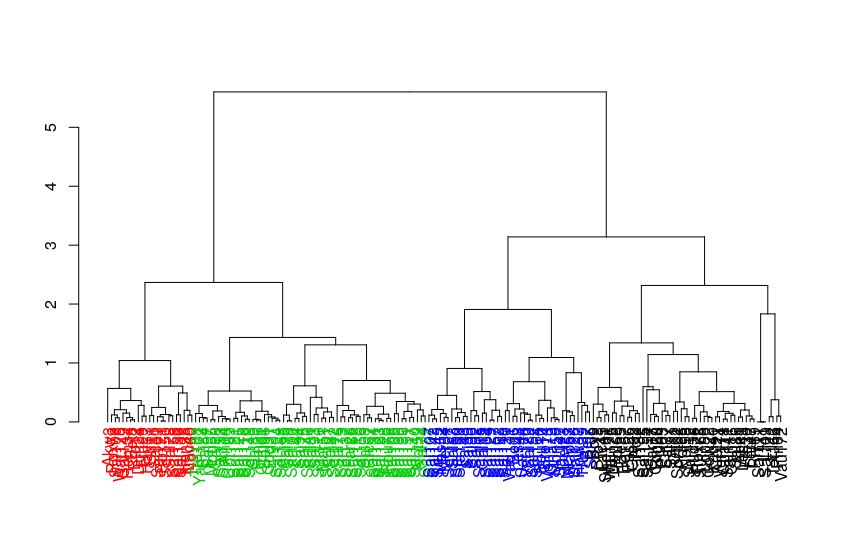
\includegraphics[width=\textwidth]{thesis/figures/clustering_trans.png}
%   \caption{Results of Ward clustering for transition data for municipalities (cut at 4 groups).}
%   \label{fig:clustertrans}
% \end{figure}

%---------------------------------------------------------------------------------------------------------------------------------------------------
% ROC Curves

% Agex

% \begin{figure}[h!]
% \makebox[\textwidth]{
%   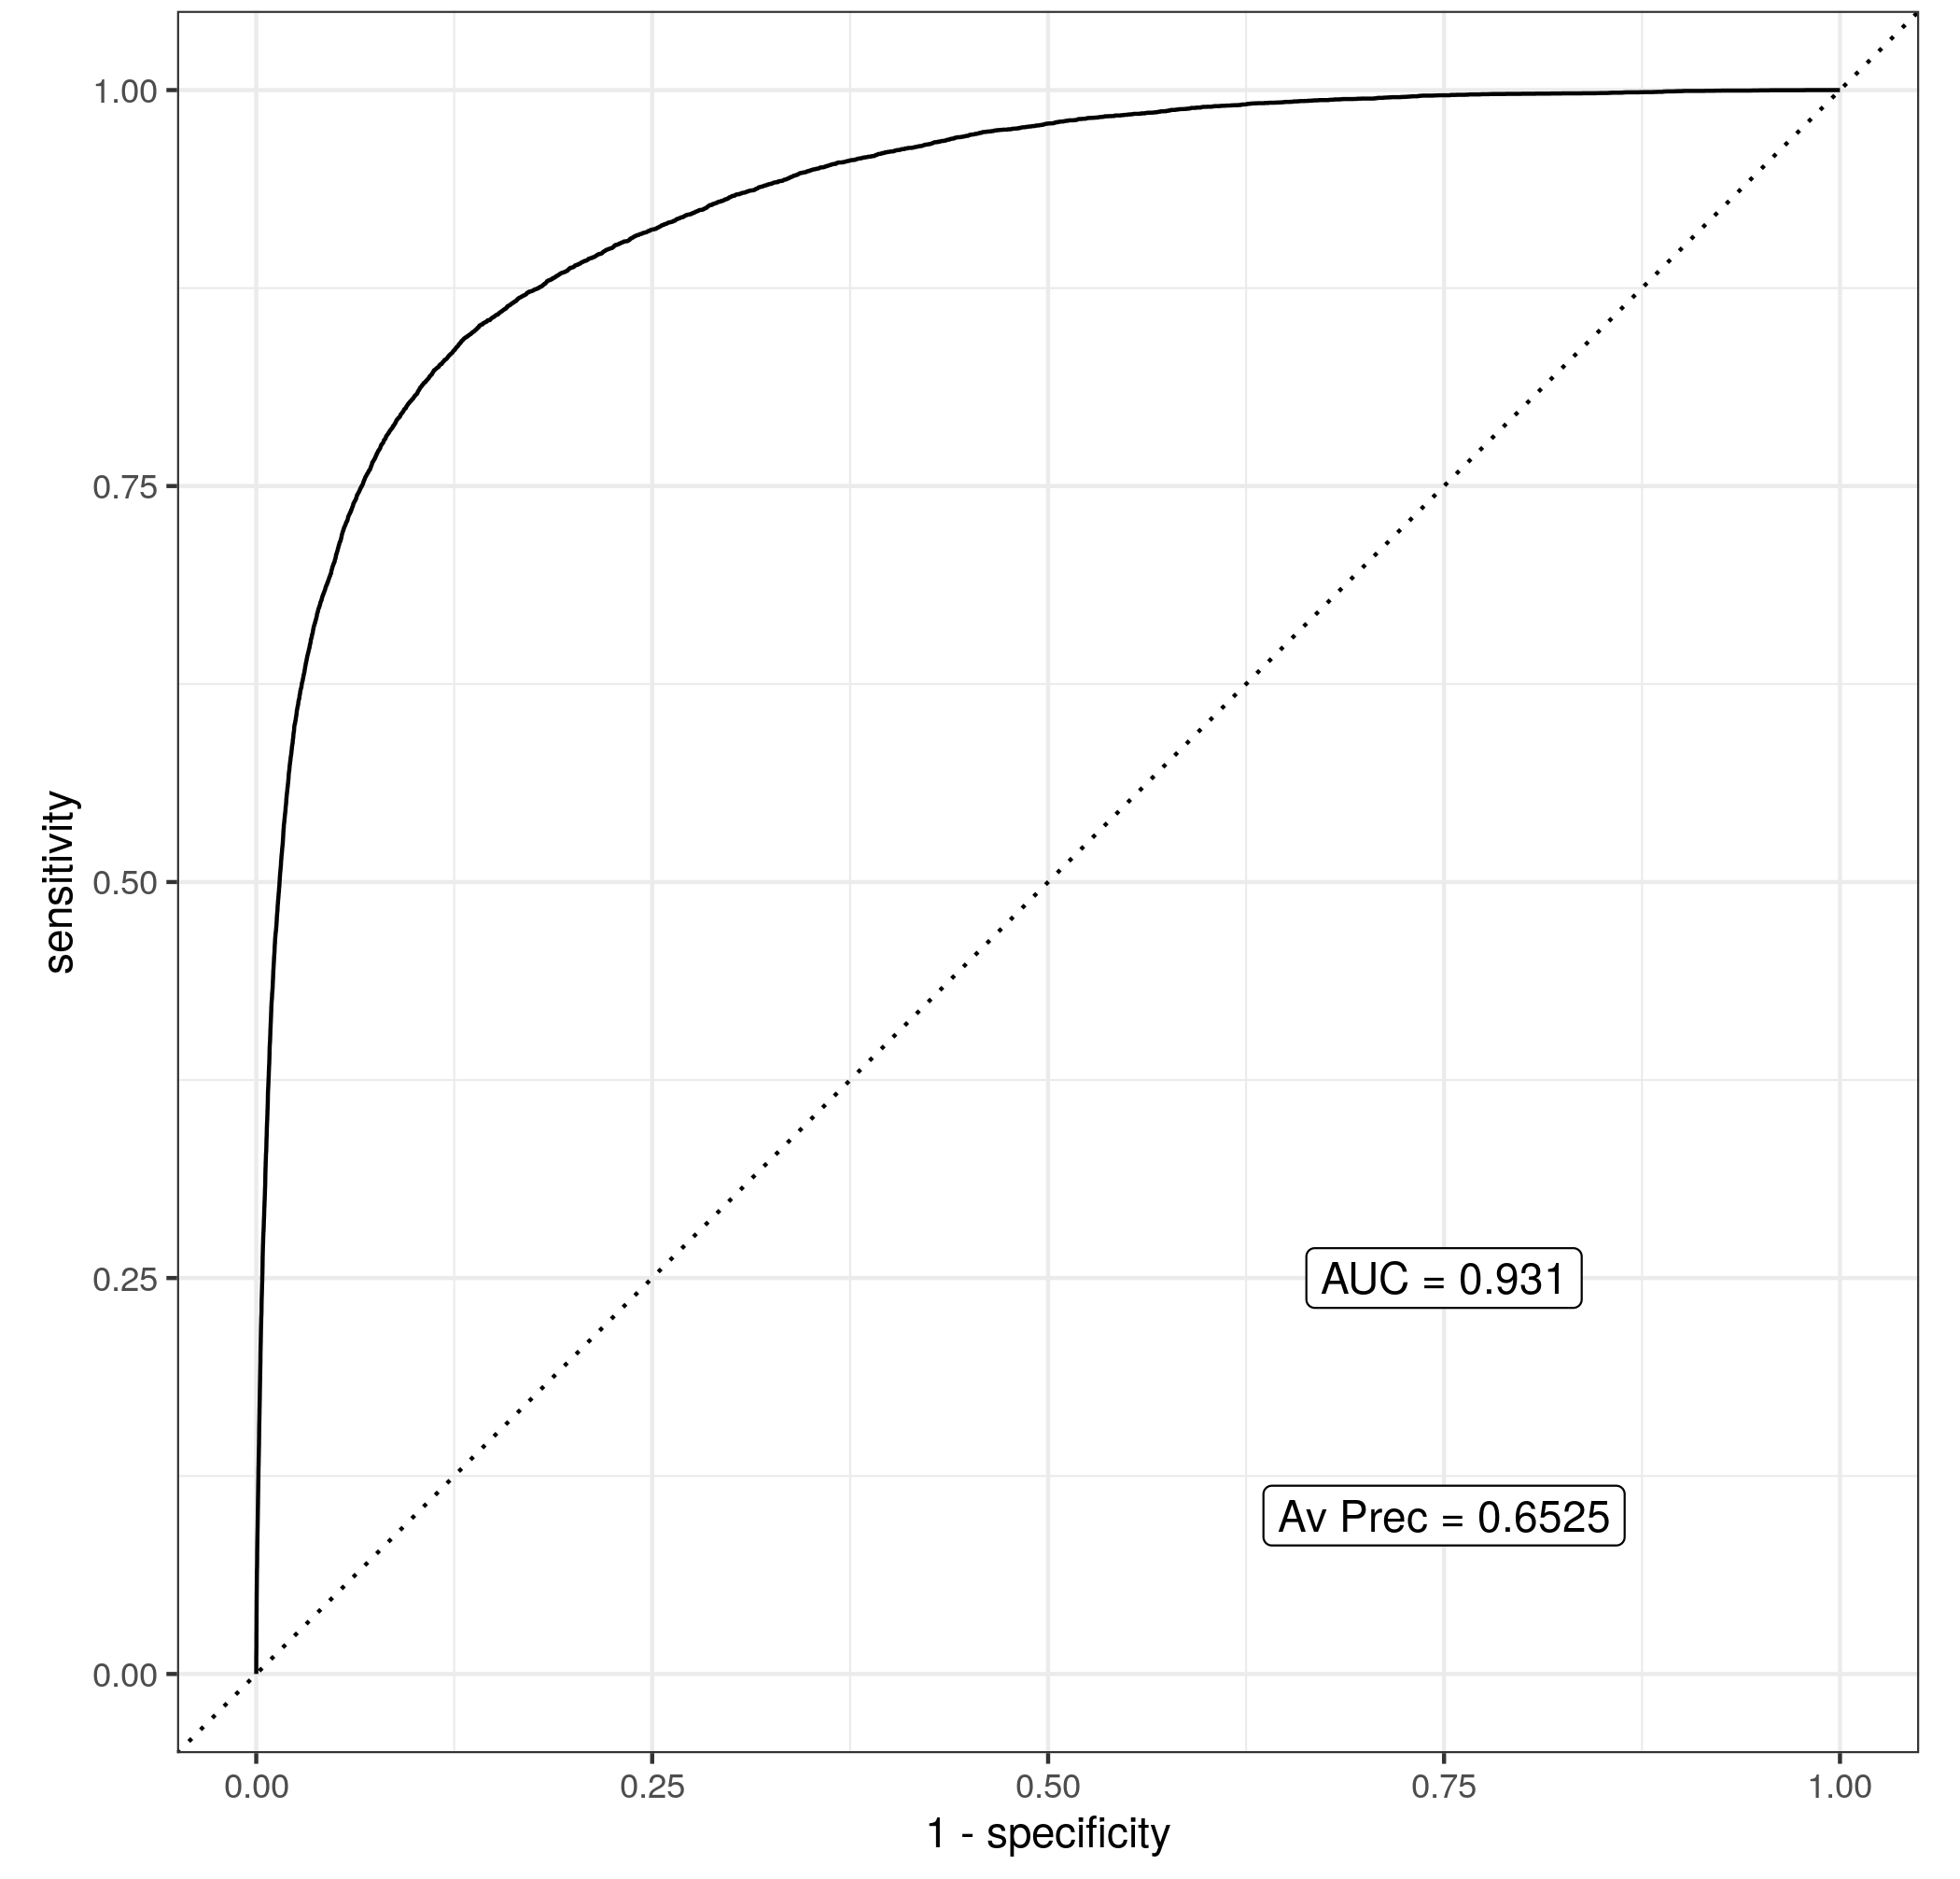
\includegraphics[width=\textwidth]{thesis/figures/rf_ratio_2_agex_roc.png}
% }
%  \caption{ROC Curve for Agricultural Expansion.}
%  \label{fig:roc_agex}
% \end{figure}
% 
% % Urb
% 
% \begin{figure}[h!]
% \makebox[\textwidth]{
%   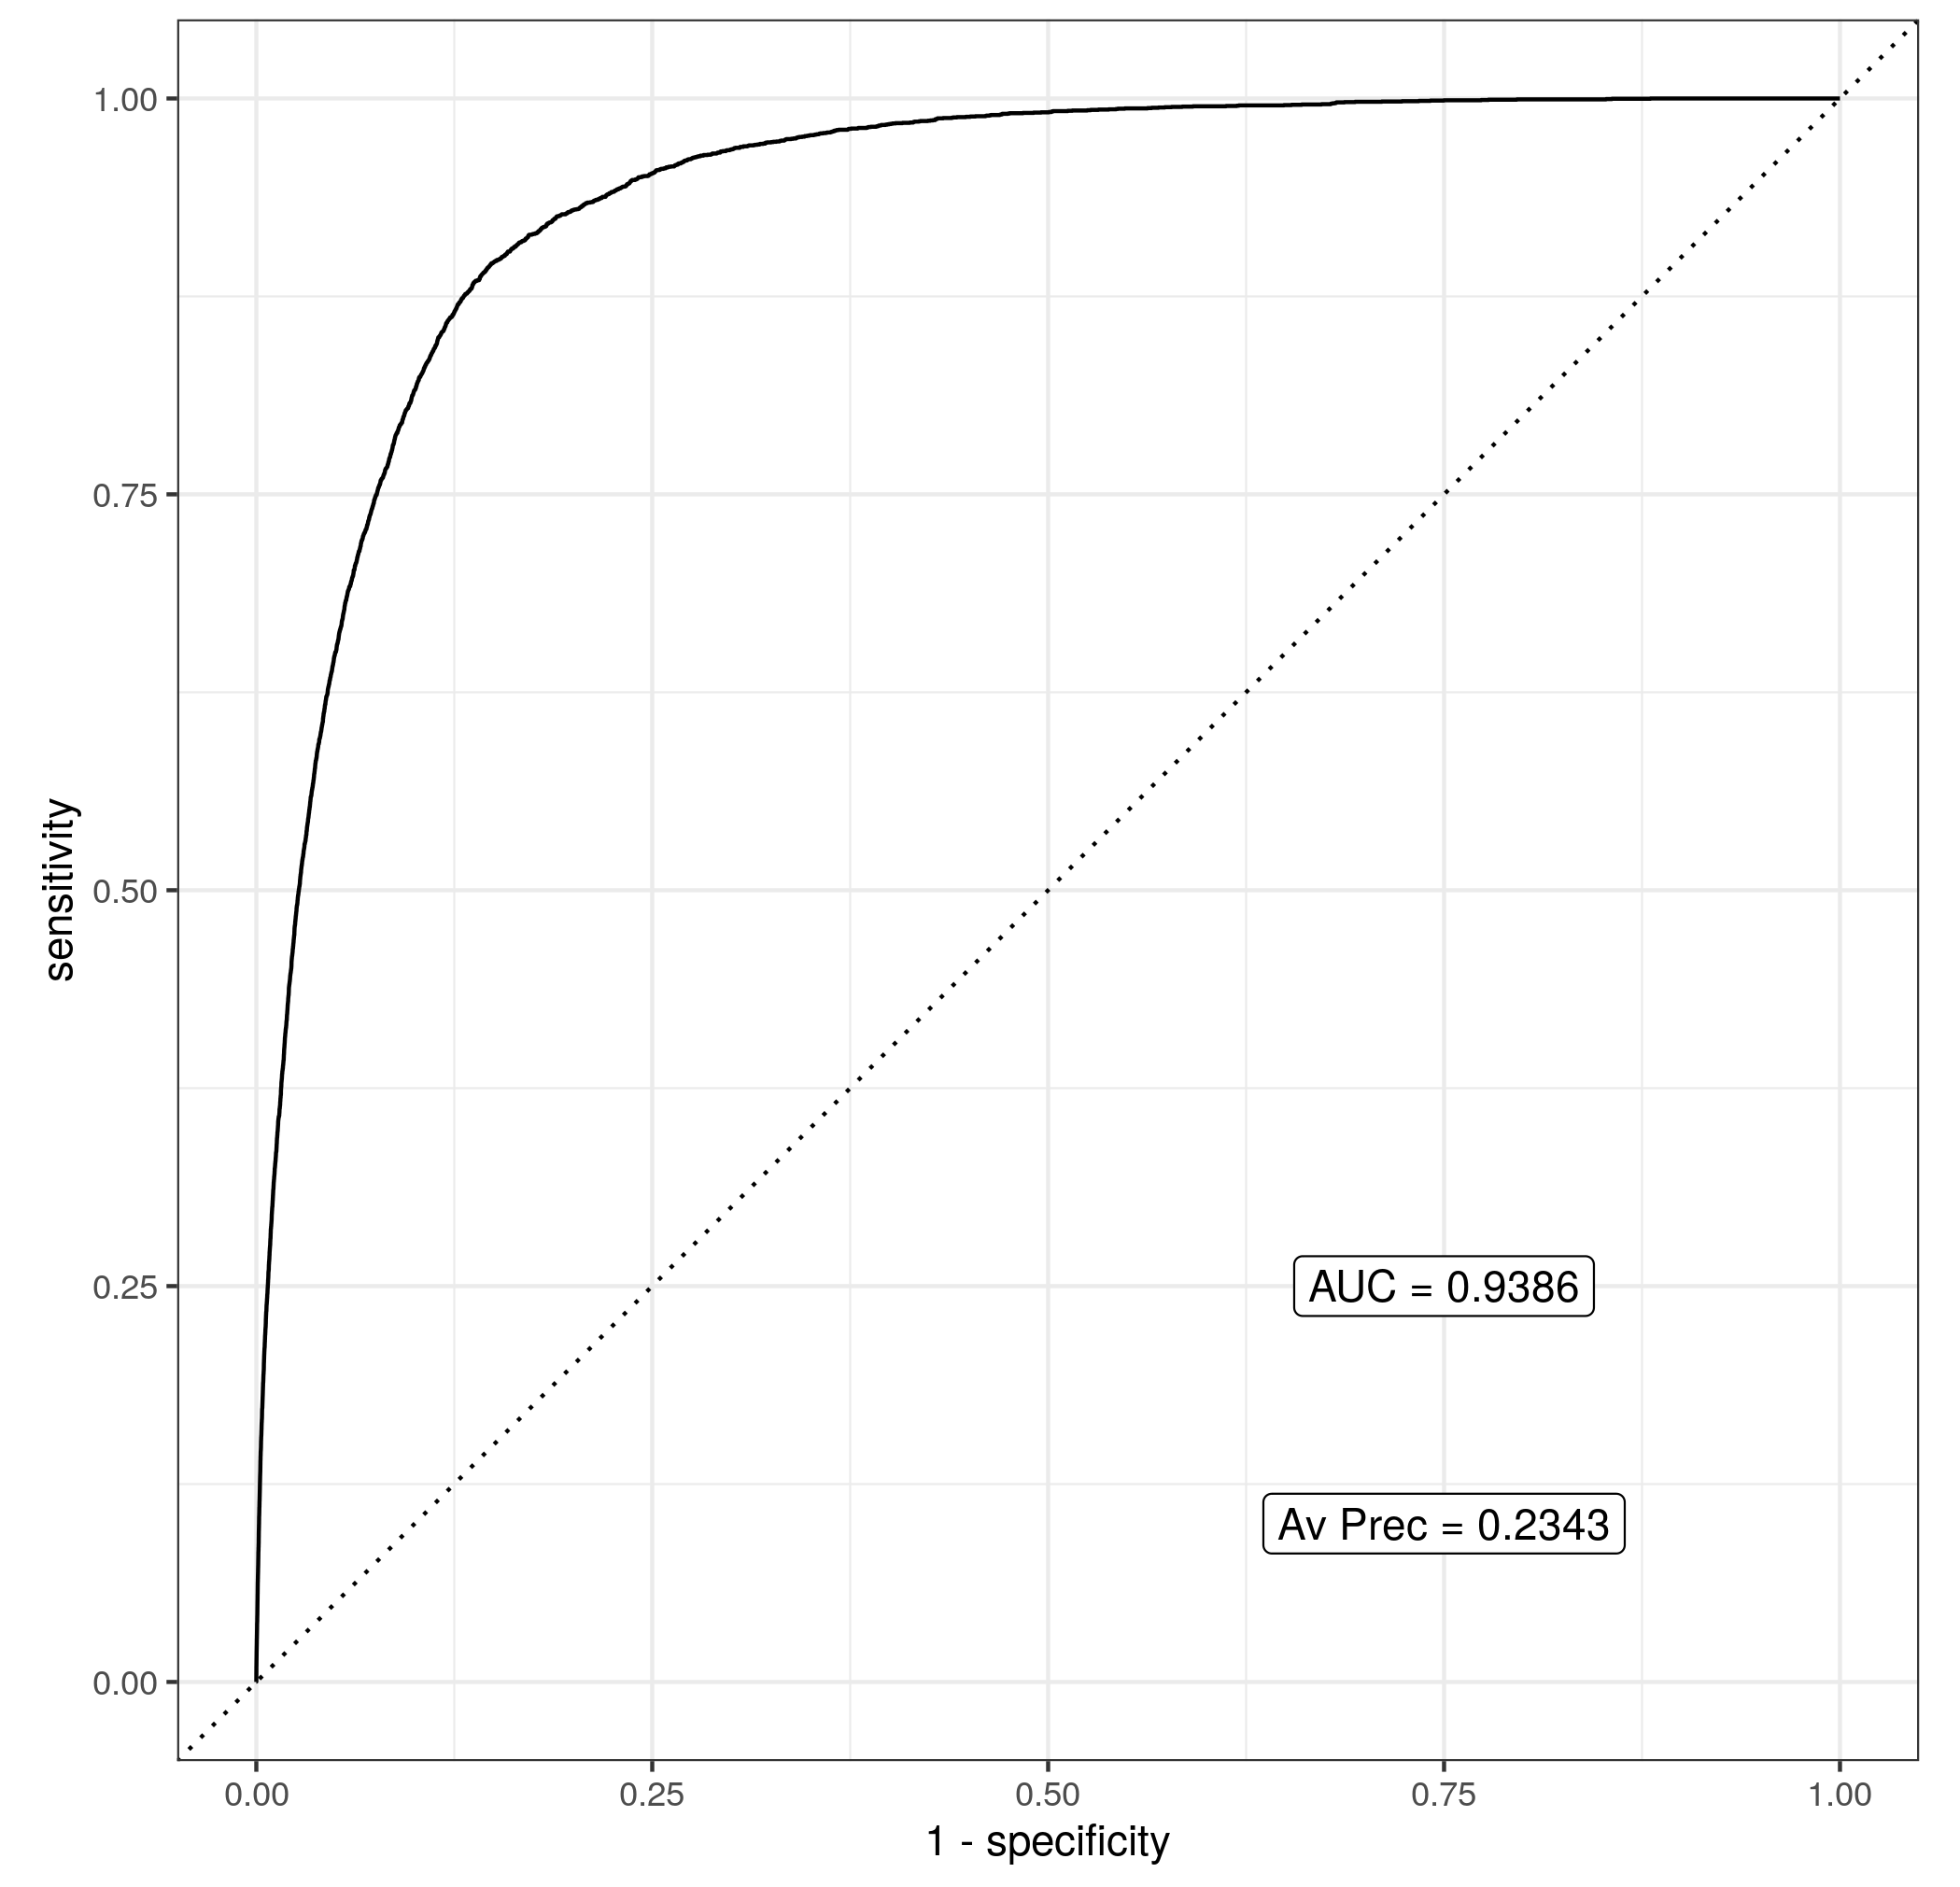
\includegraphics[width=\textwidth]{thesis/figures/rf_ratio_2_urb_roc.png}
% }
%  \caption{ROC Curve for Urbanisation.}
%  \label{fig:roc_urb}
% \end{figure}

%  Resample, figure and table

\begin{figure}[h!]
\makebox[\textwidth]{
  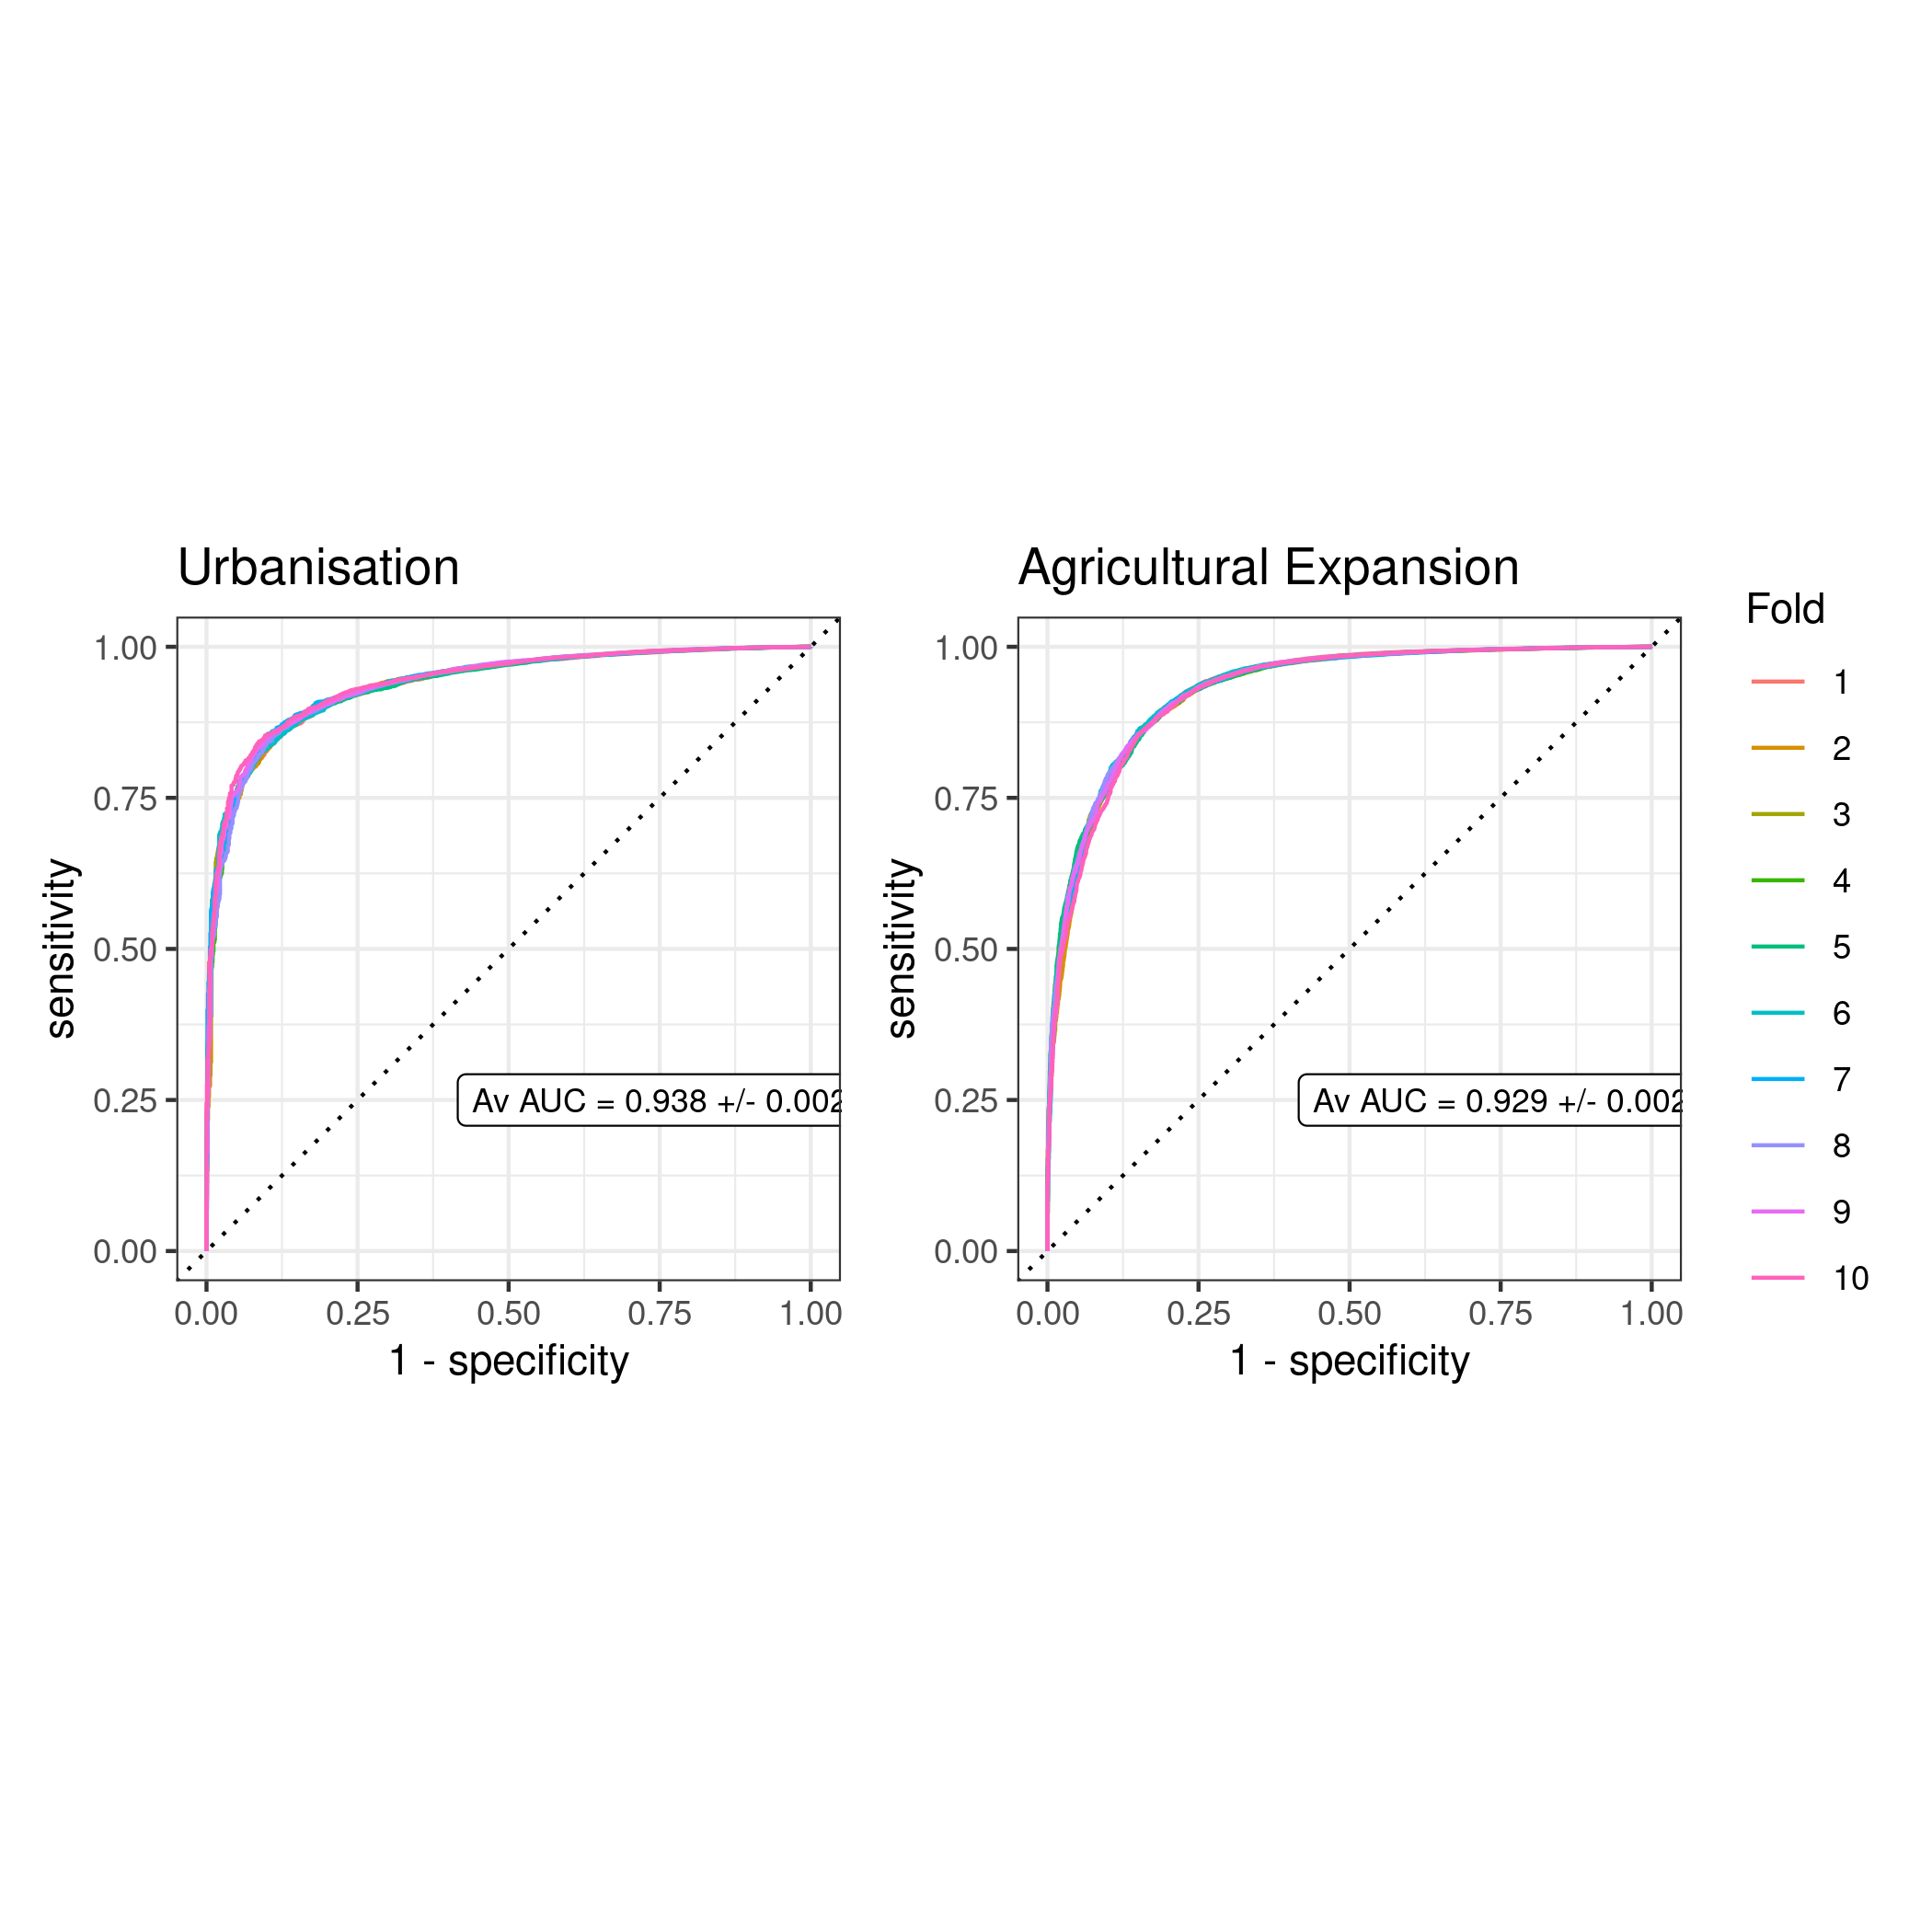
\includegraphics[width=1.3\textwidth]{thesis/figures/double_roc_resample.png}
}
 \caption[ROC Curves for re-samples for Agricultural Expansion and Urbanisation]{ROC curves (Receiver Operating Characteristic) for the results of the Random Forest models for both Agricultural Expansion and Urbanisation. Results are given for the 10 Fold CCV (Classic Cross-Validation). The average AUC (Area Under Curve) for each model (+/- standard deviation) is also given.}
 \label{fig:roc_rs}
\end{figure}

%---------------------------------------------------------------------------------------------------------------------------------------------------
% Maps compare

\begin{figure}[h!]
\makebox[\textwidth]{
  \includegraphics[width=1.3\textwidth]{thesis/figures/scenario_39_compare.png}
}
 \caption[Map of Montérégie at the beginning of the BAU scenario in 2010, and at the end in 2100 (under baseline climate scenario)]{Map of Montérégie at the beginning of the BAU (Business as Usual) scenario in 2010, and at the end of the simulation in 2100 (under baseline climate scenario)}
 \label{fig:BAU_compare}
\end{figure}

\begin{figure}[h!]
\makebox[\textwidth]{
  \includegraphics[width=1.3\textwidth]{thesis/figures/scenario_42_compare.png}
}
 \caption[Map of Montérégie at the beginning of the Reforestation scenario in 2010, and at the end in 2100 (under baseline climate scenario)]{Map of Montérégie at the beginning of the Reforestation scenario in 2010, and at the end of the simulation in 2100 (under baseline climate scenario).}
 \label{fig:Ref_compare}
\end{figure}

\newpage

%---------------------------------------------------------------------------------------------------------------------------------------------------

\chapter*{\textbf{Chapter II Supplementary Material \\ \hspace{1em}}}
\addcontentsline{toc}{section}{Chapter II Supplementary Material}

%---------------------------------------------------------------------------------------------------------------------------------------------------
% METHODS/results CHAP2

% Workshop tables

\begin{table}[h!]
\centering
\caption[Summary table of the community workshop: opportunities and challenges - non spatial elements (French)]{Summary table of the community workshop: opportunities and challenges identified by workshop participants. All non spatial elements (i.e. not mapped by participants) are listed.}
\label{tab:opp_chall_ns}
\begin{tabular}{m{0.15\textwidth}lm{0.5\textwidth}l}
\hline
\textbf{Table} &
  \textbf{\begin{tabular}[c]{@{}l@{}}Atout/Contrainte \\ (Opportunity/Challenge)\end{tabular}} &
  \textbf{\begin{tabular}[c]{@{}l@{}}Contenu\\ (Content)\end{tabular}} &
  \textbf{Score} \\ \hline
\multirow{5}{*}{Centre} &
  \multirow{3}{*}{Atouts} &
  Présence d'organisme environnementaux &
  8.00 \\ \cline{3-4} 
                       &                              & Basses terres: lien prioritaire l’échelle nationale & 4.00  \\ \cline{3-4} 
                       &                              & Programme ALUS                                      & 1.00  \\ \cline{2-4} 
                       & \multirow{2}{*}{Contraintes} & CPTAQ                                               & 18.00 \\ \cline{3-4} 
                       &                              & Besoin de rentabilité des entreprises agricoles     & 5.00  \\ \hline
\multirow{3}{*}{Est}   & Atouts                       & Vocation forestiere existante                       & 8.00  \\ \cline{2-4} 
                       & \multirow{2}{*}{Contraintes} & Tenure privée des terres                            & 2.00  \\ \cline{3-4} 
                       &                              & Plusieurs territoires couverts                      & 1.00  \\ \hline
\multirow{5}{*}{Nord} &
  \multirow{2}{*}{Atouts} &
  Réglementation favorable maintien couvert bois et corridor métropolitain &
  16.20 \\ \cline{3-4} 
                       &                              & PRMHH                                               & 10.80 \\ \cline{2-4} 
                       & \multirow{3}{*}{Contraintes} & Usage agricole prédominant                          & 44.33 \\ \cline{3-4} 
                       &                              & Compréhension et participation citoyenne            & 14.40 \\ \cline{3-4} 
                       &                              & Coûts pour faire de la connectivité                 & 10.80 \\ \hline
\multirow{6}{*}{Ouest} & \multirow{2}{*}{Atouts}      & Routes cours d'eau                                  & 3.00  \\ \cline{3-4} 
                       &                              & Presence de sols pauvre                             & 3.00  \\ \cline{2-4} 
                       & \multirow{4}{*}{Contraintes} & Les réalités économiques                            & 50.00 \\ \cline{3-4} 
                       &                              & Terres privées                                      & 12.00 \\ \cline{3-4} 
                       &                              & LPTAA                                               & 7.20  \\ \cline{3-4} 
                       &                              & Le monde politique                                  & 4.00  \\ \hline
\multirow{6}{*}{Montérégie} &
  \multirow{4}{*}{Atouts} &
  Milieu agricole: potentiel de faire des corridors si un levier est trouvé &
  12.60 \\ \cline{3-4} 
                       &                              & Présence d'acteurs locaux et éducation              & 8.00  \\ \cline{3-4} 
                       &                              & PRMHH                                               & 3.00  \\ \cline{3-4} 
                       &                              & Permettre l'aménagement forestier                   & 3.00  \\ \cline{2-4} 
                       & \multirow{2}{*}{Contraintes} & Routes et autoroutes                                & 4.00  \\ \cline{3-4} 
                       &                              & Terres privées, présence prédominantes              & 3.00  \\ \hline
\end{tabular}
\end{table}

% Opportunity /challenges

\begin{table}[]
\centering
\caption[Summary table of the community workshop: opportunities and challenges - spatial elements (French)]{Summary table of the community workshop: opportunities and challenges identified by workshop participants. All spatial elements (i.e. mapped by participants) are listed.}
\label{tab:opp_chall_s}
\begin{tabular}{m{0.15\textwidth}lm{0.5\textwidth}l}
\hline
\textbf{Table} &
  \textbf{\begin{tabular}[c]{@{}l@{}}Atout/Contrainte \\ (Opportunity/Challenge)\end{tabular}} &
  \textbf{\begin{tabular}[c]{@{}l@{}}Contenu\\ (Content)\end{tabular}} &
  \textbf{Score} \\ \hline
\multirow{5}{*}{Centre} & Atouts                       & Leaders politiques positifs                                  & 33.33          \\ \cline{2-4} 
                        & Les deux                     & Propriétés protégées                                         & 26.67          \\ \cline{2-4} 
                        & \multirow{3}{*}{Contraintes} & Pressions urbaines                                           & 42.86          \\ \cline{3-4} 
                        &                              & Manque d'adhésion des agriculteurs                           & 39.29          \\ \cline{3-4} 
                        &                              & Pressions agricoles                                          & 16.20          \\ \hline
\multirow{5}{*}{Est}          & Atouts                       & Mobilisation projet corridor bleu vert fondation séthy                         & 18.00 \\ \cline{2-4} 
                        & \multirow{4}{*}{Contraintes} & Autoroute 10                                                 & 26.67          \\ \cline{3-4} 
                        &                              & Pressions villegiatives                                      & 22.2           \\ \cline{3-4} 
                        &                              & Fragmentation des habitats liées au dev                      & 18.00          \\ \cline{3-4} 
                        &                              & Activites agricoles intensives                               & 16.2           \\ \hline
\multirow{4}{*}{Nord}         & \multirow{2}{*}{Atouts}      & Municipalite pro-protection des monteregiennes ex. st bruno mont saint hilaire & 8.00  \\ \cline{3-4} 
                        &                              & Comité municipal travail MRC MDY                             & 1.00           \\ \cline{2-4} 
                        & \multirow{2}{*}{Contraintes} & Autoroute 10 20 30 et autres                                 & 1.00           \\ \cline{3-4} 
                        &                              & Gestion de l'application des bandes riveraines               & 1.00           \\ \hline
\multirow{6}{*}{Ouest}  & \multirow{4}{*}{Atouts}      & Proximité des milieux                                        & 24.00          \\ \cline{3-4} 
                        &                              & Article 50.3 du règlement des exploitations agricoles        & 19.20          \\ \cline{3-4} 
                        &                              & Mobilisation des acteurs du milieux                          & 12.00          \\ \cline{3-4} 
                        &                              & Bande riveraine potentielle                                  & 10.00          \\ \cline{2-4} 
                        & \multirow{2}{*}{Contraintes} & Canal beauharnois isole                                      & 24.00          \\ \cline{3-4} 
                        &                              & Réticences de certains producteurs                           & 10.00          \\ \hline
\multirow{5}{*}{Montérégie 1} & \multirow{3}{*}{Atouts}      & Réseaux de sites avec couvert forestier                                        & 14.4  \\ \cline{3-4} 
                        &                              & Grande volonté d'action locale pour créer de la connectivité & 12.60          \\ \cline{3-4} 
                        &                              & Rétrécissement du fleuve                                     & 7.20           \\ \cline{2-4} 
                              & \multirow{2}{*}{Contraintes} & Agriculture intensive compenser la production                                  & 16.20 \\ \cline{3-4} 
                        &                              & Développement urbain                                         & 12.00          \\ \hline
\multirow{5}{*}{Montérégie 2} & \multirow{2}{*}{Atouts}      & Mobilisation sociale organisme conservation sensibilisation                    & 12.00 \\ \cline{3-4} 
                        &                              & Usage des sols favorable                                     & 10.00          \\ \cline{2-4} 
                        & \multirow{3}{*}{Contraintes} & Prix des terres agricoles                                    & 12.00          \\ \cline{3-4} 
                        &                              & Étalement urbain deuxième couronne                           & 10.00          \\ \cline{3-4} 
                        &                              & Pole logistique de transport                                 & 10.00          \\ \hline
\end{tabular}
\end{table}

\begin{table}[h!]
\centering
\caption[Administrative districts (MRCs) covered by each table in the workshop]{Breakdown of the administrative districts (MRCs, Municipalité Regionales de Comté) covered by each table in the workshop.}
\label{tab:workshoptables}
\begin{tabular}{ll}
\hline
\textbf{Table} & \textbf{MRCs} \\ \hline
Ouest (West) & Vaudreuil, Haut SL, Beauharnois \\
Centre (Center) & Jardins, Haut Richelieu, Rouville, Roussillon \\
Nord (North) & \begin{tabular}[c]{@{}l@{}}Longueuil, Marguerite d'Youville, Vallée du richelieu, \\ Pierre de Saurel, Les Maskoutains\end{tabular} \\
Est & Brome-Missisquoi, Haute Yamaska, Acton \\
Transversal (x2) & Toute la Montérégie (All of  Montérégie)\\ \hline
\end{tabular}
\end{table}

%---------------------------------------------------------------------------------------------------------------------------------------------------
% Maps compare

\begin{figure}[h!]
\makebox[\textwidth]{
  \includegraphics[width=1.3\textwidth]{thesis/figures/scenario_45_compare.png}
}
  \caption[Map of Montérégie at the beginning of the Corridor protection scenario in 2010, and at the end in 2100 (under baseline climate scenario)]{Map of Montérégie at the beginning of the Corridor protection scenario in 2010, and at the end of the simulation in 2100 (under baseline climate scenario).}
 \label{fig:Corr_compare}
\end{figure}

\begin{figure}[h!]
\makebox[\textwidth]{
  \includegraphics[width=1.3\textwidth]{thesis/figures/scenario_48_compare.png}
}
  \caption[Map of Montérégie at the beginning of the Corridor protection + Reforestation scenario in 2010, and at the end in 2100 (under baseline climate scenario)]{Map of Montérégie at the beginning of the Corridor protection + Reforestation scenario in 2010, and at the end of the simulation in 2100 (under baseline climate scenario).}
 \label{fig:	CorrRef_compare}
\end{figure}

\begin{figure}[h!]
\makebox[\textwidth]{
  \includegraphics[width=1.3\textwidth]{thesis/figures/scenario_51_compare.png}
}
  \caption[Map of Montérégie at the beginning of the Corridor protection + Targeted Reforestation scenario in 2010, and at the end in 2100 (under baseline climate scenario)]{Map of Montérégie at the beginning of the Corridor protection + Targeted Reforestation scenario in 2010, and at the end of the simulation in 2100 (under baseline climate scenario).}
 \label{fig:	CorrRefT_compare}
\end{figure}

%---------------------------------------------------------------------------------------------------------------------------------------------------
% Flow

% Radar All
\begin{figure}[h!]
\makebox[\textwidth]{
  \includegraphics[width=1.3\textwidth]{thesis/figures/radar_ggradar_both.png}
}
  \caption[Radar graph of change in mean flow (decrease in \% of the baseline 2010 flow) between 2010 (observed) and 2100 (predicted), comparing all scenarios]{Radar graph of change in mean flow (decrease in \% of the baseline 2010 flow) between 2010 (observed) and 2100 (predicted). This compares all scenarios, for all 5 species. Note that the line color represent species and that each side of the graph is a different scenario.}
 \label{fig:flow_radar_both}
\end{figure}
% !TEX root = ./thesis.tex

\chapter*{\textbf{Appendix 2: Workshop Materials \\ \hspace{1em}}}
\addcontentsline{toc}{chapter}{Appendix 2: Chapter II Workshop Materials}

\setcounter{chapter}{4}
\setcounter{table}{0}
\setcounter{figure}{0}

\begin{itemize}
  \item \textbf{Feuille de route du Participant - Workshop participant roadmap} - This is the document that was given to each participant during the workshop. It contains helpful information meant to guide them during the exercises: the agenda for the day, a few illustrations of simple connectivity concepts, and suggestions of assets and obstacles to connectivity.
  % \item \textbf{Document du facilitateur - Facilitator's sheet} - This is the document that was given to each facilitator. It contains guidelines for leading the conversation at each table and at each step of the workshop.
  % This needs to be removed for final submission.
  % \item \textbf{Certificate of Ethical Acceptability of Research Involving Humans} - This document certifies that this research project was approved by McGill's university Research Ethics Board Office.
\end{itemize}

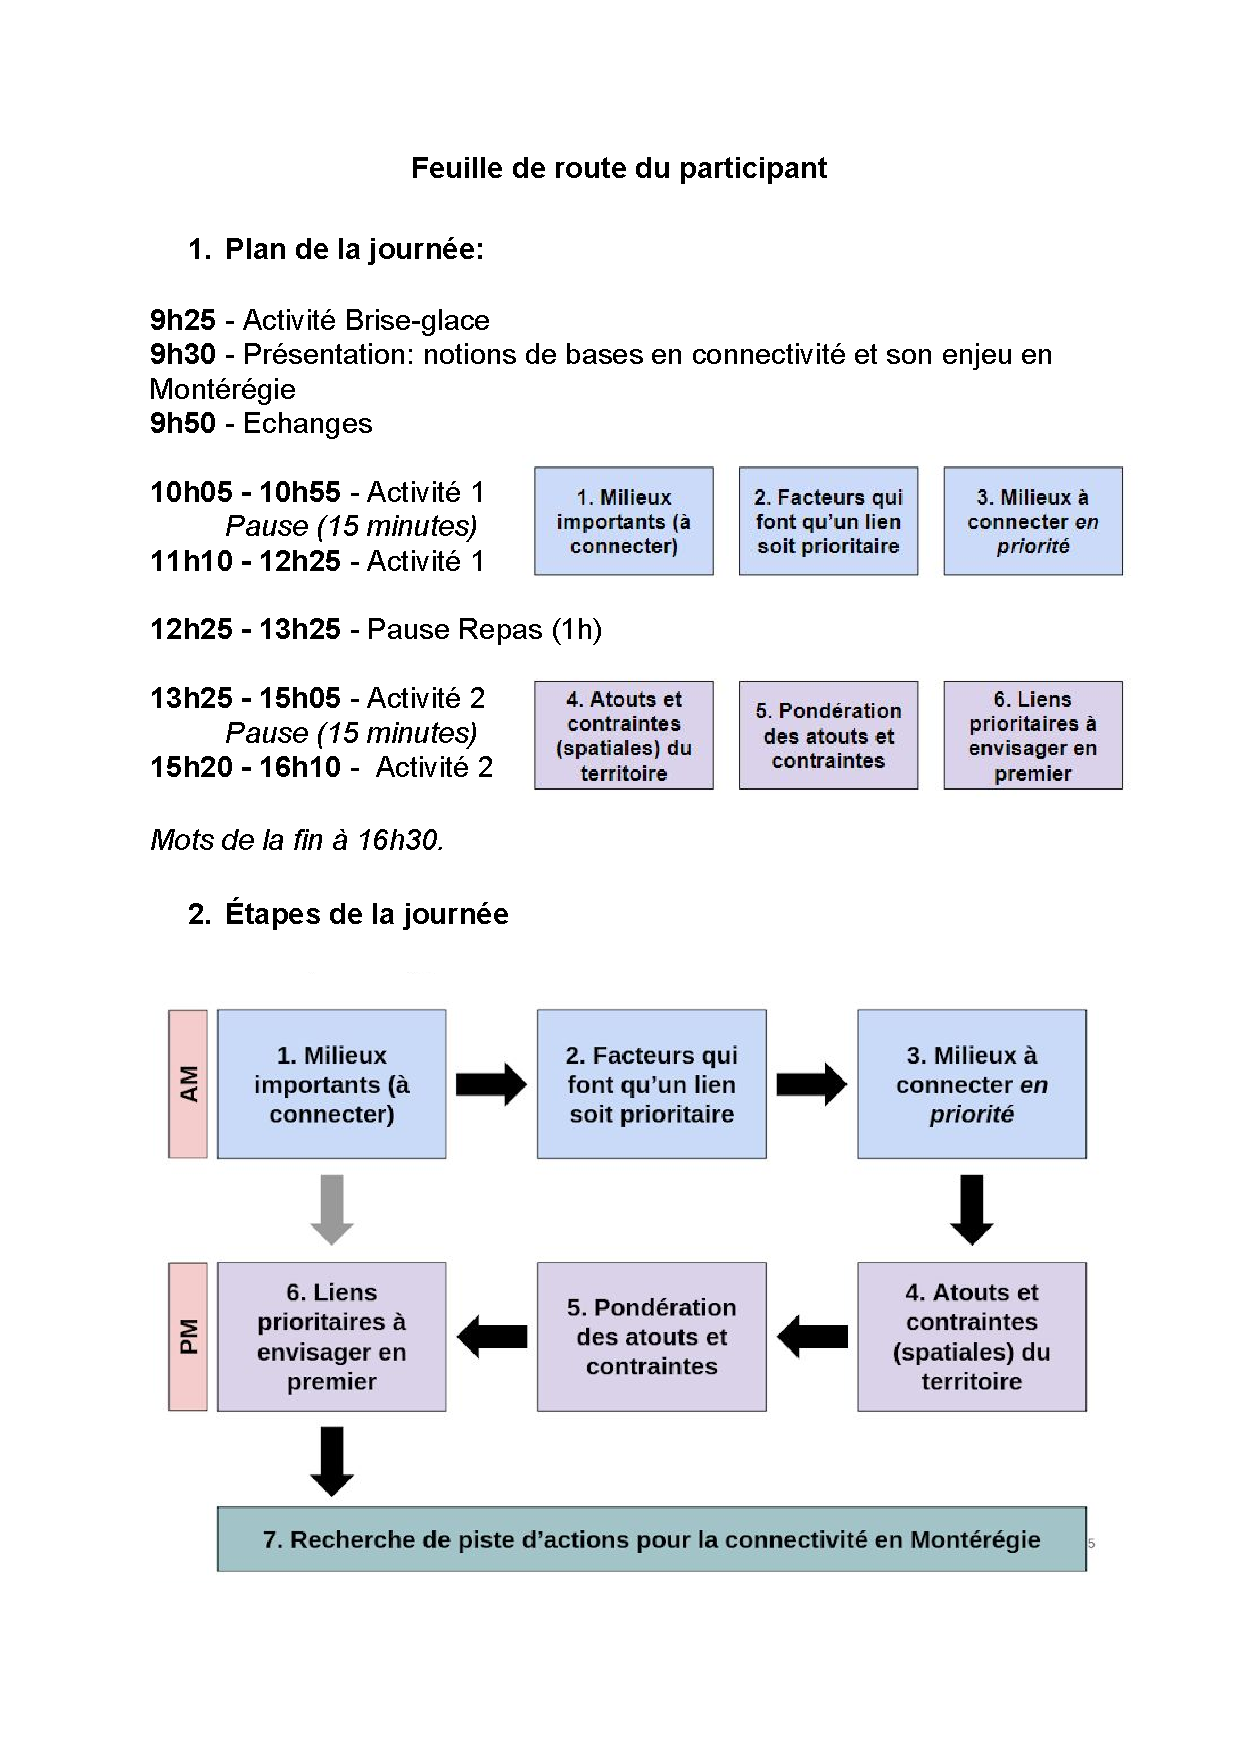
\includepdf[pages=-,pagecommand={},width=1.3\textwidth]{thesis/appendix/Cahier_du_Participant.pdf}
% \includepdf[pages=-,pagecommand={},width=1.3\textwidth]{thesis/appendix/Document_du_facilitateur.pdf}
% 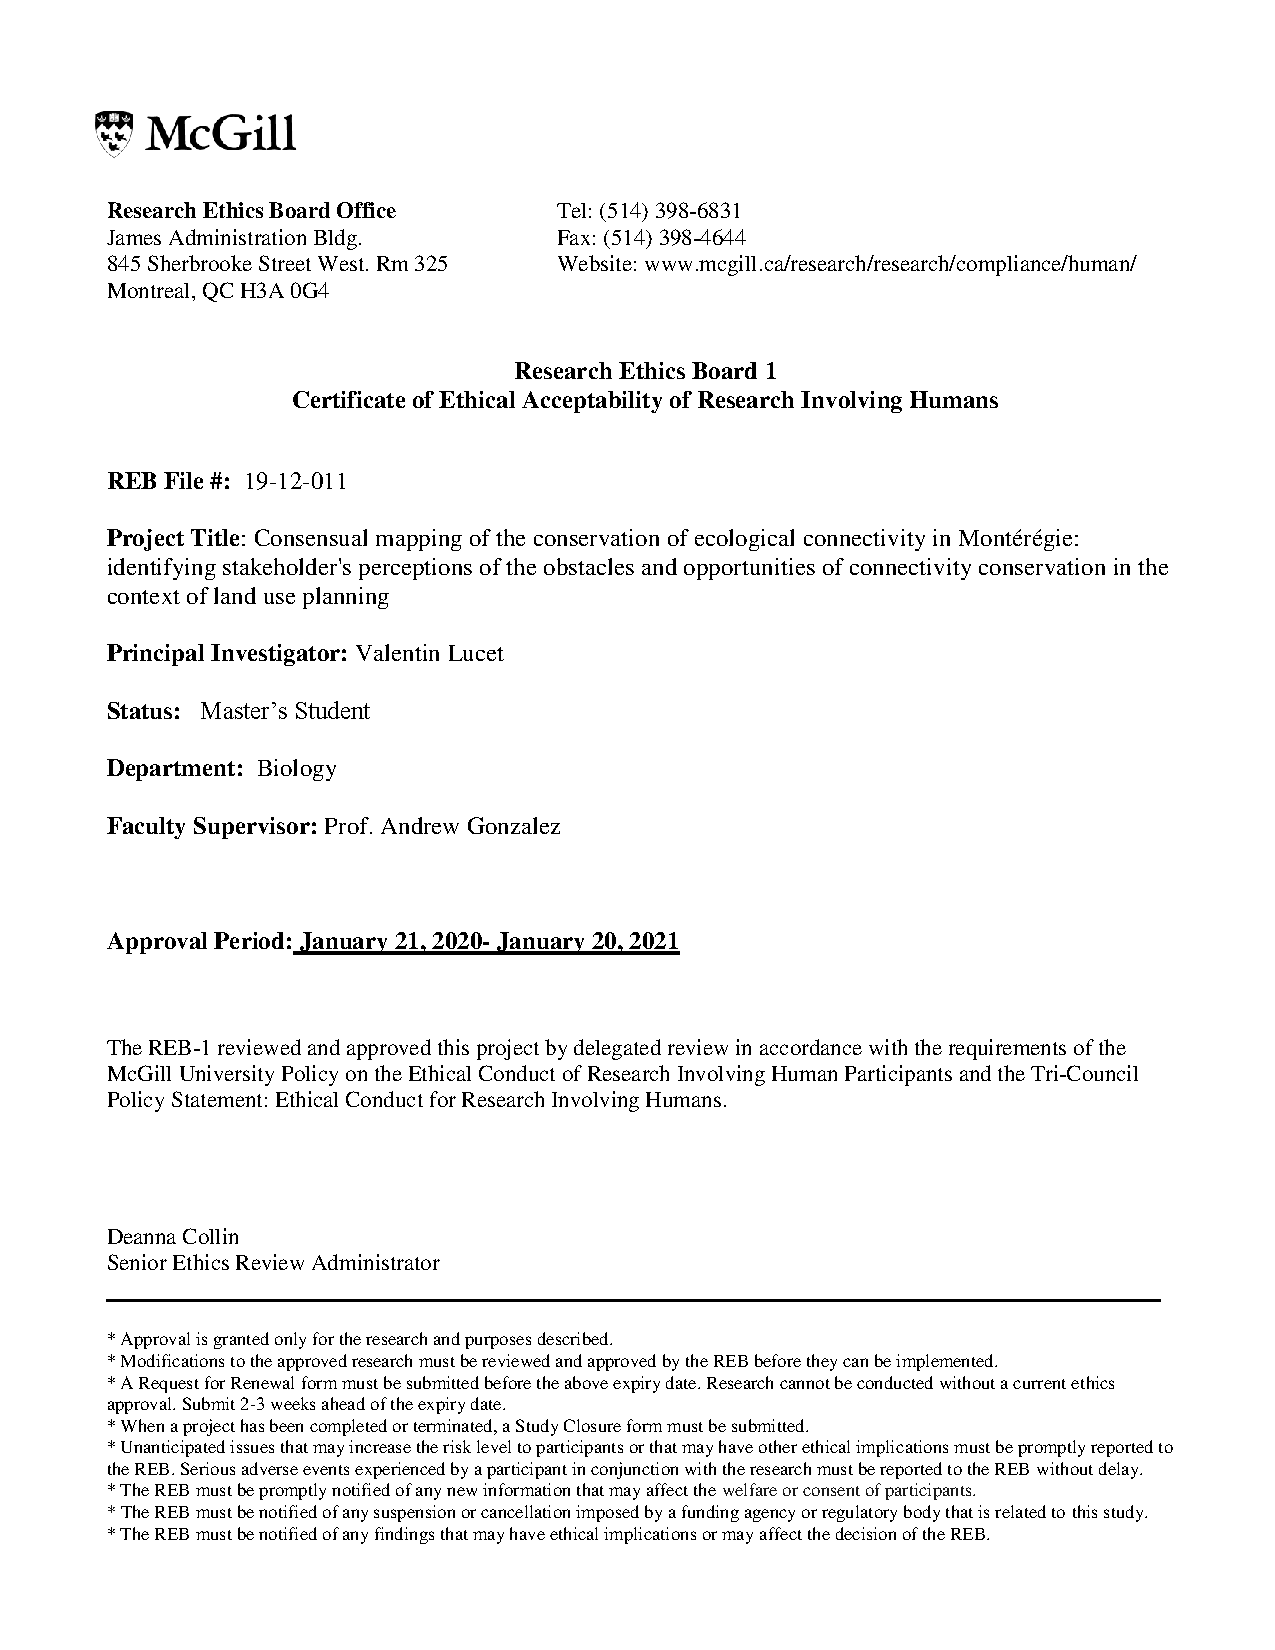
\includepdf[pages=-,pagecommand={},width=1.3\textwidth]{thesis/appendix/Ethics_approval_Lucet.pdf}
% !TEX root = ./thesis.tex

\chapter*{\textbf{Supplementary analysis of land use change in Monteregie \\ \hspace{1em}}}
\addcontentsline{toc}{chapter}{Appendix 4: Supplementary analysis of land use change in Monteregie}

\setcounter{chapter}{5}
\setcounter{table}{0}
\setcounter{figure}{0}

%----------------------------------------------------------------------------------------------------------------

% Figures: values

% Clustering moved to appendix

% PCA
\begin{figure}[h!]
\makebox[\textwidth]{
  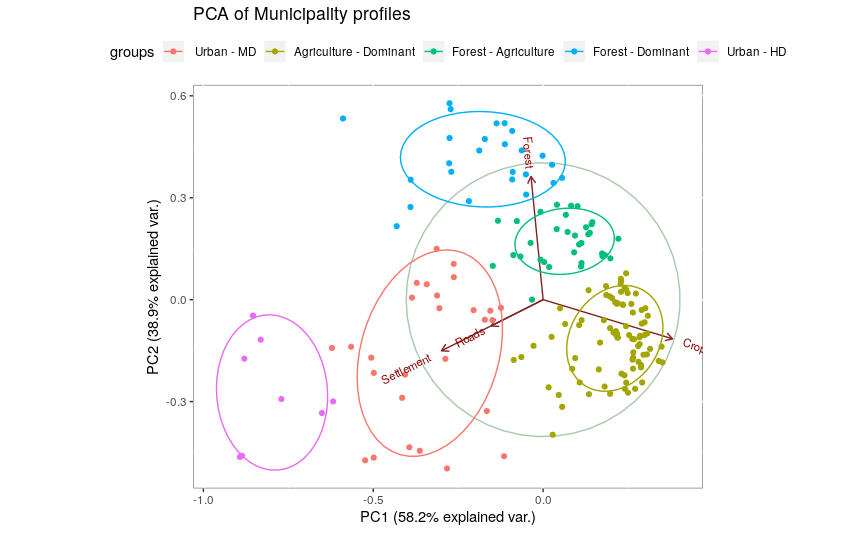
\includegraphics[width=0.8\textwidth]{thesis/figures/PCA_data_profiles.png}
}
\caption{Ordination of land use data (proportions) for municipalities.}
\label{fig:PCAvals}

% MAP
\makebox[\textwidth]{
    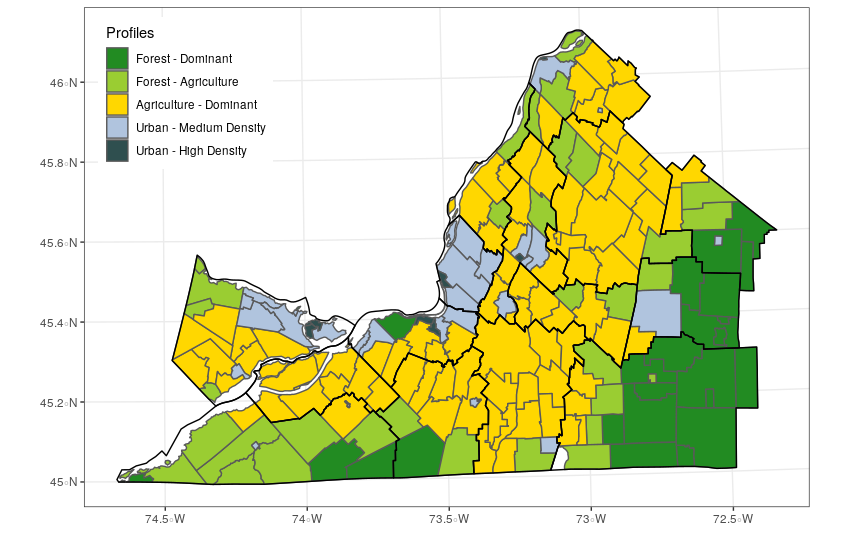
\includegraphics[width=0.8\textwidth]{thesis/figures/profiles_land_use.png}
}
\caption{Geographical distribution of the 5 profiles identified in figure \ref{fig:PCAvals}.}
\label{fig:mapvals}
\end{figure}

% Figures: Transitions

% PCA
\begin{figure}[h!]
\makebox[\textwidth]{
  \includegraphics[width=0.8\textwidth]{thesis/figures/PCA_trans_profiles.png}
}
\caption{Ordination of land use transition data for municipalities.}
\label{fig:PCAtrans}

%MAP
\makebox[\textwidth]{
    \includegraphics[width=0.8\textwidth]{thesis/figures/transition_prof_map.png}
}
\caption{Geographical distribution of the 4 change profiles identified in figure \ref{fig:PCAtrans}.}
\label{fig:maptrans}
\end{figure}

\clearpage

%\ETDAppendix{References}{
%\printbibliography
%}
\printbibliography[heading=bibintoc, section=0, title={General Bibliography \vspace{1em}}]

\end{document}
